\documentclass{overturerepchap}
%**********************************************************
%
% Bibliography support
%
%**********************************************************
%\def\@reportno{YY--NN}		% default report no.
%\def\reportno#1{\gdef\@reportno{#1}}

\newcommand{\bthisbibliography}[1]{\section*{References}%
   \begin {list} {}%
     {\settowidth {\labelwidth} {[#1]XX}%
      \setlength {\leftmargin} {\labelwidth}%
      \addtolength{\leftmargin} {\labelsep}%
      \setlength {\parsep} {1ex}%
      \setlength {\itemsep} {2ex}%
     }
  }
\newcommand{\ethisbibliography}{\end{list}}
\newcommand{\refitem}[2]
  {\bibitem[#1]{#2}}

\newcommand{\back}{$\setminus$}
\newcommand{\RuleTarget}[1]{\hypertarget{rule:#1}{}}
\newcommand{\Ruledef}[2]
{
  \RuleTarget{#1}\Rule{#1}{#2}%
  }
\newcommand{\Ruleref}[1]{
  \hyperlink{rule:#1}{#1}}
\newcommand{\Lit}[1]{`{\tt #1}\Quote}
\newcommand{\Rule}[2]{
  \begin{quote}\begin{tabbing}
    #1\index{#1}\ \ \= = \ \ \= #2  ; %    Adds production rule to index
    
  \end{tabbing}\end{quote}
  }
\newcommand{\SeqPt}[1]{\{\ #1\ \}}
\newcommand{\lfeed}{\\ \> \>}
\newcommand{\dsepl}{\ $|$\ }
\newcommand{\dsep}{\\ \> $|$ \>}
\newcommand{\Lop}[1]{`{\sf #1}\Quote}
\newcommand{\blankline}{\vspace{\baselineskip}}
\newcommand{\Brack}[1]{(\ #1\ )}
\newcommand{\nmk}{\footnotemark}
\newcommand{\ntext}[1]{\footnotetext{{\bf Note: } #1}}
\newlength{\kwlen}
\newcommand{\Keyw}[1]{\settowidth{\kwlen}{\tt #1}\makebox[\kwlen][l]{\sf
    #1}}
\newcommand{\keyw}[1]{{\bf\ttfamily{#1}}}
\newcommand{\id}[1]{{\tt #1}}
\newcommand{\metaiv}[1]{\begin{alltt}\input{#1}\end{alltt}}

\newcommand{\OptPt}[1]{[\ #1\ ]}
\newcommand{\MAP}[2]{\kw{map }#1\kw{ to }#2}
\newcommand{\INMAP}[2]{\kw{inmap }#1\kw{ to }#2}
\newcommand{\SEQ}[1]{\kw{seq of }#1}
\newcommand{\NSEQ}[1]{\kw{seq1 of }#1}
\newcommand{\SET}[1]{\kw{set of }#1}
\newcommand{\PROD}[2]{#1 * #2}
\newcommand{\TO}[2]{$#1 \To #2$}
\newcommand{\FUN}[2]{#1 \To #2}
\newcommand{\PUBLIC}{\ifthenelse{\boolean{VDMpp}}{public\mbox{}}{\mbox{}}}
\newcommand{\PRIVATE}{\ifthenelse{\boolean{VDMpp}}{private}{\mbox{}}}
\newcommand{\PROTECTED}{\ifthenelse{\boolean{VDMpp}}{protected}{\mbox{}}}
\newcommand{\vdmtools}{VDMTools}
\newcommand{\VDMTools}{VDMTools}
\newcommand{\vdmpp}{VDM++} %{\small VDM}$^{++}$}
\usepackage{multicol}
\newcommand{\showtrace}{RealTime Log Viewer}
\usepackage{makeidx}

\usepackage{graphicx, color}

% definition of VDM++, JavaCC, JJTree, JTB, ANTLR and SableCC for listings
\newcommand{\NL}{\mbox{}\\ \vspace*{-5mm}}
\usepackage{listings}
\newcommand{\url}[1]{\texttt{#1}}
\usepackage{hyperref}

\usepackage{times}
\usepackage{color}
\lstdefinelanguage{VDM++}
  {morekeywords={act, active, fin, req, waiting, abs, all, allsuper, always, and, answer, 
     assumption, async, atomic, be, bool, by, card, cases, char, class, comp, compose, conc, cycles,
     dcl, def, definitions, del, dinter, div, dlmodule, do, dom, dunion, duration, effect, elems, else, elseif, end,
     error, errs, exists, exists1, exit, exports, ext, floor, for, forall, from, functions, 
     general, hd, if, imports, in, inds, infer, init, inmap, input, instance, int, inter, inv, inverse, iota, is, 
     isofbaseclass, isofclass, inv, inverse, lambda, len, let, map, measure, mu,
     mutex, mod, module, nat, nat1, new, merge, 
     munion, not, of, operations, or, others, per, periodic, post, power, pre, pref, 
     private, protected, public, qsync, rd, responsibility, return, reverse,  
     sameclass, parameters, psubset, rem, renamed, rng, sel, self, seq, seq1, set, skip, specified, st, 
     start, startlist, state, static, subclass, subset, subtrace, sync, system, then, thread, 
     threadid, time, tixe, tl, to, token, traces, trap, types, undefined,
     union, uselib, using, values, 
     variables, while, with, wr, yet, RESULT, false, true, nil, periodic pref, rat, real},
   %keywordsprefix=mk\_,
   %keywordsprefix=a\_,
   %keywordsprefix=t\_,
   %keywordsprefix=w\_,
   sensitive,
   morecomment=[l]--,
   morestring=[b]",
   morestring=[b]',
  }[keywords,comments,strings]
\lstdefinelanguage{JavaCC}
  {morekeywords={options, PARSER\_BEGIN, PARSER\_END, SKIP, TOKEN},
   sensitive=false,
  }[keywords]

% define the layout for listings
\lstdefinestyle{tool}{basicstyle=\ttfamily,
                         frame=trBL, 
			 showstringspaces=false, 
			 frameround=ffff, 
			 framexleftmargin=0mm, 
			 framexrightmargin=0mm}
\lstdefinestyle{mystyle}{basicstyle=\footnotesize\ttfamily,
                         frame=trBL, 
%                         numbers=left, 
%			 gobble=0, 
%			 basewidth=0.51em,
                         showstringspaces=false, 
%			 linewidth=\textwidth, 
			 frameround=fttt, 
			 aboveskip=2mm,
			 belowskip=2mm,
			 framexleftmargin=0mm, 
			 framexrightmargin=0mm}
%\lstdefinestyle{mystyle}{basicstyle=\sffamily\small,
%			 frame=tb,
%                         numbers=left,
%			 gobble=0,
%			 showstringspaces=false,
%			 linewidth=345pt,
%			 frameround=ffff,
%			 framexleftmargin=8mm,
%			 framexrightmargin=8mm,
%			 framextopmargin=1mm,
%			 framexbottommargin=1mm,
%			 aboveskip=7mm,
%			 belowskip=5mm,
%			 xleftmargin=10mm,}

\lstset{style=mystyle}
\lstset{language=VDM++}
%\lstset{alsolanguage=Java}
% The command below enables you to escape into normal LaTeX mode inside your 
% VDM chunks by starting with a `!' character and ending with a `!'
\lstset{escapeinside=!!}

%This file has been converted to use LaTeX2e
%\documentstyle[overture]{article}
%
% any "\include{...}" statements go here
%
\include{ifad}
\include{graphics}
\usepackage{cite}
\usepackage{alltt}
%\usepackage{fancyhdr}
\renewcommand{\topfraction}{0.9}
\renewcommand{\textfraction}{0.05}
\renewcommand{\floatpagefraction}{0.9}
\makeindex

\begin{document}
\title{Development Process of Distributed Embedded Systems using VDM}
\author{Peter Gorm Larsen and Sune Wolff \\ 
Department of Engineering, Aarhus University\\
Finlandsgade 22, DK-8200 \AA{}rhus N, Denmark\\[3mm]
Nick Battle\\
Fujitsu Services\\
Lovelace Road, Bracknell, \\
Berkshire. RG12 8SN, UK\\[3mm]
John Fitzgerald and Kenneth Pierce\\
School of Computing Science\\
Newcastle University\\
UK
}
\date{September 2013}

\reportno{TR-006}     

\maketitle


{\textbf{Document history}}

\begin{tabular}{|l|l|l|l|}\hline
Month   & Year & Version & Version of Overture.exe \\ \hline
April   & 2010 &   & 0.2   \\ \hline
May     & 2010 & 1 & 0.2 \\ \hline
February& 2011 & 2 & 1.0.0\\ \hline
September& 2013 & 3 & 2.0.0\\ \hline
\end{tabular}

\tableofcontents

\chapter*{Preface}

This document is intended to provide readers who already have
experience with general VDM concepts from language manuals
\cite{LangManPP} or books \cite{Fitzgerald&05} and/or courses and it
is also assumed that the reader has general knowledge about concepts
using for concurrent systems
\cite{Ben-Ari82,Hoare85,Chandy&88,Milner89,Lea99}. From a tool perspective
it is also assumed that the readers are already familiar with the
basic functionality from Overture (\url{http://www.overturetool.org}) 
%and/or \VDMTools\
%(\url{http://www.vdmbook.com/tools.php)} 
and a UML tool such as Modelio (\url{www.modelio.org}).
%Enterprise Arhictect (\url{http://www.sparxsystems.com/})
%or Rational Rose (\url{http://www-306.ibm.com/software/rational/}).

VDM \cite{Jones90a,Dawes91,Fitzgerald&98,Fitzgerald&08c} is a formal method
\cite{Craigen&93b,Hinchey&95,Woodcock&09} and these are characterized by being
able to express things in an abstract fashion and having a precise
semantics for the models produced in these languages. Three different
dialects exists for VDM;
VDM-SL, VDM++ and VDM-RT \cite{Larsen&10b}. Some of these
methods include methodological steps of getting from a very abstract
model to a more concrete model. This process is typically referred to
as refinement \cite{Jones90a,Morgan90a,Woodcock&96,Back&98} when formal
relationships are included between the different models. In this
document no claims are made between the different models so no formal
refinement will be included.

This document is structured such that all readers with advantage can
read the introduction in Chapter~\ref{chap:intro} first. In case the
reader have limited experience and knowledge about synchronization of
concurrent systems it may be an advantage then to just to
Chapter~\ref{chap:sync} to get more knowledge about that before
proceeding with the main process guidelines for the development of
real-time systems in Chapter~\ref{chap:process}. The process is followed
by a major example that is developed according to the guidelines
presented in Chapter~\ref{chap:example}. Understanding that requires
knowledge about both VDM and general concurrency principles. All the 
different models for the example used in this document are also available
on-line from \url{www.vdmbook.com} so it is possible for the reader to 
get hands-on experience with them.

In 
Chapter~\ref{chap:period} periodic threads and statically schedulable
systems are treated. Chapter~\ref{chap:schedule} provides insight 
into the scheduling principles that can be used for the execution of
concurrent and for distributed VDM-RT models in Overture. In 
Chapter~\ref{chap:timetrace} it is presented how post-execution analysis
can be made of timed logfiles produced by Overture during execution 
of a scenario (primarily using the \showtrace). 
Finally, Chapter~\ref{chap:postscript} rounds off the document with a 
postscript indicating what the reader should have obtained at this point.


\chapter{Introduction}\label{chap:intro}

This document describes the envisaged process by which reactive
distributed embedded real-time
systems could be developed using Overture. In particular, the
document describes how key features of real-time systems can be
modelled and analyzed using tool support.  In this document the main
focus is on the different activities performed during the analysis and
design phases of the development process. Thus, the implementation
phase of the traditional waterfall life cycle \cite{Royce70} is not
dealt with in detail in this document. However, the use of Overture
does not require the use of the waterfall life cycle and thus parts of
the guidelines can be selected on a needs basis.

\section{Characteristics of Reactive Real-Time Systems}

Reactive real-time systems possess a number of unique characteristics
which means that conventional (formal and informal) approaches to
modelling and analysis are inadequate. That is, in addition to
conventional functional correctness (correctness of computed values),
other factors can influence whether the software is defined in such a
way that the overall system performs correctly, and are therefore
challenges to the system developer. These challenges are a result of
the reactive, concurrent and real-time nature of such systems, so the
challenges intrinsic to each of these kinds of system are
described. Often it is simply not possible to check whether a system
design will be adequate before it is fully implemented and operating
in its real environment. For a number of critical systems this is
unacceptably late and this document describes how one can get a higher
level of confidence in the correctness of a design using Overture.

\subsection{Challenges of Reactive Systems}

Reactive systems are often \emph{closed loop} systems. That is, they
typically repeatedly take data from sensors and compute commands for
actuators based on this data. The behaviour of the actuators then
influences the values read by the sensors. In order to appropriately
model this feedback loop one needs to have an accurate model of the
environment in order to be able to validate that the system will work
correctly in its expected environment. Moreover reactive systems are
typically non-terminating, so traditional formal methods approaches
dealing with total correctness (formal proof of an algorithm always 
satisfying certain formally defined conditions) are not appropriate. 

Modelling the environment behaviour may not be convenient in a
discrete event formalism such as VDM. Often a detailed description of
physical world entities are more conveniently created using different
bases in mathematics such as differential equations. Thus, in case the
fidelity of the requirements are sufficiently high it will be optimal
to have the environment (the physical system to be controlled) and the
system to be developed (the controller of the physical system) be
described in different formalisms which can be combined for example
using co-simulation \cite{Broenink&10,Fitzgerald&13b}. However in this document the
environment will be modelled using VDM for simplicity reasons. We will
also discuss under which circumstances a multi-disciplinary models
will be advantagous. The DESTECS (Design Support and Tooling for
Embedded Control Software) project (\url{http://www.destecs.org}) was
targeted explicitly at this combination and thus
complementary methodology documentation came out of that project (and its tool
support is now called \textbf{Crescendo}.

Reactive systems need to be able to cope with \emph{random events} that might
occur in the environment. This means that the modelling of the
environment need to incorporate sporadic events. The challenge here is
also to be able to handle all possible ways in which the environment
can behave, and appropriately document the assumptions made about this 
behaviour. For critical applications the handling of erroneous
situations typically take up the majority of the effort in the
development of an appropriate controller.

\subsection{Challenges of Concurrency}

The correctness of a concurrent system can often be dependent on the
kind of \emph{scheduling} algorithm used, and the manner in which the
scheduling algorithm is used. In order to be able to predict whether a
particular design will work correctly for different scenarios one
needs to take scheduling into account. In addition to scheduling the 
mastering of synchronisation between different threads adds to the
complexity of concurrency.

\subsection{Challenges of Real-Time}

Real-time systems sometimes need to meet \emph{hard deadlines}. That
is, failure to meet a deadline could lead to the system's mission
being compromised. Any kind of analysis which can indicate scenarios
where such deadlines cannot be met is extremely valuable.  Typically,
the performance of a small portion of the system can critically affect
the ability of the system to meet its deadlines. Such portions are
referred to as \emph{bottlenecks}.  The earlier potential bottlenecks
can be pinpointed the better.

Real-time systems often need to meet \emph{soft deadlines}. That is,
deadlines which, if met late, will not cause system failure, but
persistent lateness could cause degraded performance. Detection of
this is similar to the hard deadlines above; the value of this is
necessarily smaller but still important.

Real-Time systems need to be able to cope with periodic events which
do not occur perfectly periodically. This is called jitter and the
acceptable level for this is dependent upon the different design
decisions made.

\subsection{Challenges of Distribution}

From a system perspective it is often advantageous to structure an 
embedded system on a number of processors. A part of the distribution
of functionality to be performed by such a system is more or less
determined by the physical structure of the system and its interaction
with the environment. However, for a significant portion of the desired 
functionality the system architect have a challenging task determining 
how to allocate different parts of the functionality to different 
computation units. It requires a lot of skill to become convinced
about the chosen architecture living up to different kinds of timing 
requirements with a given collection of processors with physical 
characteristics for example in the form of speed and memory. 

In order to find an optimal system architecture it is an advantage
to experiment with commonly used scenarios with different combinations of 
different processors and different allocations of functionality to 
these processors. The development guidelines presented in this document
aims to provide an ability for carrying out such experiments early in
the life-cycle without having to invest in the real hardware with 
different capabilities for processor speeds. Naturally it is still just a
model but it is taking the speed of the processors and the bus capacities 
into account so it should at least be able to provide pretty good guidance
about an optimal system architecture. The things that are left out of
the modelling here are memory and optimisation techniques such as caching
and pipelining.

\section{Overview of VDM and its tool support}

In this section we give a brief description of those features of VDM
dialects specifically suited to modelling real-time systems and
deployment to multiple processors. A more substantial overview of the
VDM languages can be found in \cite{LangManPP}.

VDM++ is a model-based object-oriented specification language. It
permits description of concurrent models by using threads. Real-time
behaviour of models can be analyzed dynamically. A VDM++ model is
organized as a collection of classes. A class may contain values,
types, instance variables, functions and operations. Note that
functions are not allowed to read or write instance variables, whereas
operations are.

Overture is a tool suite which support amongst other
things, static analysis of models (syntax and type checking), and
execution of models with dynamic type analysis (invariant checking,
pre- and post-condition checking). In addition Overture and
\vdmtools\ have features enabling users to move back and forth between
a graphical UML view and a textual detailed VDM++ view. As described
in \cite{Guidelines}, this allows the complementary benefits of UML
and VDM to be exploited.

A variety of scheduling algorithms are supported by Overture,
and during model execution, information on the real-time behaviour of
the model is accumulated for post-execution analysis. More details of
how Overture facilitates timing analysis is given in
Section~\ref{sec:timingintro}. For post-execution analysis there is also
a feature in Overture
called \showtrace\ that may be used. More details will be
provided about that in Chapter~\ref{chap:timetrace}.

We now describe four key features of VDM-RT used when modelling
real-time systems: 
\begin{enumerate}
\item threads,
\item duration and cycles statements,
\item system and environment and
\item deployments.
\end{enumerate}

\subsection{Threads}

A thread is an entity within a class. It is used to model independent
behaviour. That is, a thread represents activity within a system,
whereas a class without a thread is more akin to a server, passively
responding to requests. Thus when a class containing a thread
definition is instantiated, a thread is created. However this thread
may only be scheduled when it is explicitly started using a VDM++
{\bf\ttfamily{start}} statement. Consider the following example where a class
\texttt{A} has a thread that is started inside an operation called 
\texttt{op} in a class called \texttt{B}:
%\newpage

\begin{multicols}{2}
\begin{lstlisting}
class A

instance variables
  i : nat := 0

thread
  while i < 10 do
    i := i + 1

end A
\end{lstlisting}
\begin{lstlisting}
class B

operations

op : () ==> ()
op() ==
( dcl a : A := new A();
  start(a)
)
end B
\end{lstlisting}
\end{multicols}

In this example, the thread for object \texttt{a} will not be available for
scheduling until the statement {\bf\ttfamily{start}}\texttt{(a)} 
has been executed.

Threads may be either procedural or periodic. A procedural thread is
simply a statement (as the while loop in the above example), which is
executed to completion subject to scheduling and descheduling. A
periodic thread has the form

\begin{lstlisting}
periodic (!\textit{period},\textit{jitter},\textit{delay},\textit{offset}!) (!\textit{operation}!)
\end{lstlisting}

A periodic thread is started in the same way as a procedural thread,
using a {\bf\ttfamily{start}} statement. The operation stated in the thread
declaration is then executed repeatedly, with frequency determined by
\texttt{period}. If \texttt{jitter} is allowed it means that the period 
is not perfectly periodic, but may vary with the amount of
\texttt{jitter} before and after the ideal periodic time. If there is
a minimal arrival time between two periodic event that is indicated by
the \texttt{delay} parameter. Finally, in case the periodic occurrence
should not start right when the periodic thread is started it is
possible to use the \texttt{offset} parameter to describe
that. Examples of all of this will follow.

Being a bit more precise we can consider Figure~\ref{fig:perioddef} and
state that:
\begin{itemize}
\item \textbf{period} is a non-negative, non-zero value
that describes the length of the time interval between
two adjacent events in a strictly periodic event stream
(where $jitter=0$)
\item \textbf{jitter} is a non-negative value that describes
the amount of time variance that is allowed around a single
event. We assume that the interval is balanced $[-j,j]$.
Note that jitter is allowed to be bigger than the period
to characterize so-called event bursts.
\item \textbf{delay} is a non-negative value smaller than
the period which is used to denote the minimum inter arrival
distance between two adjacent events.
\item \textbf{offset} is a non-negative value which is used
to denote the absolute time value at which the first period
of the event stream starts. Note that the first event
occurs in the interval $[$\texttt{offset, offset + jitter}$]$.
\end{itemize}

\begin{figure}[!htb]
\begin{center}
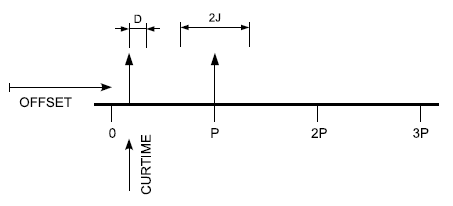
\includegraphics[width=4in]{figures/PeriodJitterDelayOffset.PNG}
\end{center}
\caption{Example of a periodic event stream with a $(p,j,d,o)$-tuple\label{fig:perioddef}}
\end{figure}

Communication between threads is based on shared objects. Thus a
synchronization mechanism is necessary to ensure integrity of shared
objects. This mechanism is described in Chapter~\ref{chap:sync}.

\subsection{Duration and Cycles Statements}

A duration statement is a VDM-RT statement that allows a fixed estimate to
be placed on the execution time of a particular portion of a model. A
duration statement has the form

\begin{lstlisting}
duration (!\textit{t}!) !\textit{statement}!
\end{lstlisting}

This means that \emph{statement} is estimated to take \emph{t} nanoseconds 
to execute. This information is used for accumulation of
real-time behaviour; details of this accumulation, and the manner in
which time is to be interpreted are described in
Section~\ref{sec:timingintro} below.  Otherwise the duration statement
has the exact functional effect of its body \textit{statement}.

A cycles statement is a VDM-RT statement that allows a relative
estimate to be placed on the execution of a particular portion of a
model relative to the \texttt{CPU} it is allocated to (deployed). A cycles
statement has the form

\begin{lstlisting}
cycles (!\textit{instruction cycles}!) !\textit{statement}!
\end{lstlisting}

This means that \emph{statement} is estimated to take
\emph{instruction cycles} to execute on any platform. Thus, if a
processor with double processor speed is chosen it will take half the
time. This information is used for accumulation of real-time
behaviour; details of this accumulation, and the manner in which time
is to be interpreted are described in Section~\ref{sec:timingintro}
below.  Otherwise the cycles statement has the exact functional
effect of its body \textit{statement}.

\subsection{The System and the Environment}

In order to be able to describe distributed systems in \vdmpp\
includes a notion of a system that describes how different parts of
the system modelled are deployed to different Central Processing Units
(\texttt{CPU}'s) and communication \texttt{BUS}'es 
connecting the \texttt{CPU}'s
together. Syntactically the system is described exactly like ordinary
classes, except that the keyword ``\keyw{system}'' instead of the
keyword ``\keyw{class}''.

The special thing about the system is that it can make use of special
implicitly defined classes called \texttt{CPU} and \texttt{BUS}. It is 
not possible to create instances of the system, but instances made of
\texttt{CPU} and \texttt{BUS} will be created at initialisation time. 
Note that \texttt{CPU} and \texttt{BUS} cannot be used outside the
system definition.

The instances of \texttt{CPU} and \texttt{BUS} must be made as instance 
variables and the definition must use constructors. The constructor for the
\texttt{CPU} class takes two parameters: the first one indicate the 
primary scheduling policy used for the \texttt{CPU} whereas the second 
parameter provides the capacity of the \texttt{CPU} (indicated as number of 
instructions Per Second or Hz - NB. the step size of time is 1 nanosecond). 
The constructor for the \texttt{BUS}
class takes three parameters. The first one indicates the kind of bus, the
second one the capacity of the bus (its band width in bytes per second) and finally the third 
parameter gives a set of \texttt{CPU} instances connected together by the
given \texttt{BUS} instance.

The currently supported primary scheduling policies for the \texttt{CPU}
are:
\begin{description}
\item[\texttt{<FP>}:] Fixed Priority. If this scheduling policy is
  used the cpu scheduler will examine the threads with the highest
  priority first to see if they are ready to be executed or they are
  blocked for some reason (a synchronisation constraint or by an
  operation call on a different cpu).
\item[\texttt{<FCFS>}:] First Come First Served. If this scheduling
  policy is used the cpu scheduler will always swap between threads in
  a round-robin fashion starting with the first one created. Each
  thread will be allowed to continue its execution for a time limit
  (decided by the user) before the next thread is examined. In this
  way fairness will be ensured at normal cpus but for threads running
  at the virtual cpu (where time is not incremeneted based on
  instruction execution) no fairness is ensured since ian infinite
  loop here may take over the entire execution.
\end{description} 

The currently supported primary scheduling policies for the \texttt{BUS}
are (however, in this version all of them are treated as FCFS):
\begin{description}
%\item[\texttt{<TDMA>}:] Time Division Multiple Access
\item[\texttt{<FCFS>}:] First Come First Served
%\item[\texttt{<CSMACD>}:] Carrier Sense Multiple Access with Collision 
%                          Detection
\end{description} 

Note that the principles used for describing the system to be developed using 
the VDM technology may be copied for the environment as well. This means that
it is possible to use the ``\keyw{system}'' keyword also for the environment as
a whole and thus be able to accurately describe the interaction between the
system and its environment. In case this is not done virtual processors 
(\texttt{CPU}'s)
and a virtual communication channel (a \texttt{BUS}) 
are established for each of the
environment instances created inside the special class ``\texttt{World}''
that describe the composition of systems.

\subsection{Deployments}

The \texttt{CPU} class has member operations called \texttt{deploy} and
\texttt{setPriority}. The \texttt{deploy} operation takes one parameter
which must be an object that is declared as a static instance variable
inside the system. The semantics of the deploy operation is that execution
of all functionality inside this object will take place on the 
\texttt{CPU} that it
has been deployed to. The \texttt{setPriority} operation takes two 
parameters where the first must be the name of a public operation that 
has been deployed to the \texttt{CPU}
 and the second parameter is a natural number.
The semantics of the \texttt{setPriority} operation is that the given 
operation is assigned the given priority (the second parameter). This will
be used when fixed priority scheduling is used on the given
\texttt{CPU}. For operations that are used on a \texttt{CPU} using
fixed priority scheduling that has \textbf{not} been assigned a value
using the \texttt{setPriority} operation a default priority of 1 is
assigned to it. The same holds for normal theads in active classes.

\section{Timing Analysis}\label{sec:timingintro}

The objective when performing timing analysis using Overture is to
identify potential performance bottlenecks. That is, to identify
those portions of the model that could cause scheduling problems
and/or failure to meet deadlines. This allows the feasibility of a
particular \emph{dynamic architecture} to be examined. A dynamic
architecture is a design which has been decomposed into a number of
processes or threads onto a number of processors.

%% The interpreter developed for
%% Overture follows the final principles from the PhD thesis from Marcel
%% Verhoef \cite{Verhoef08} by Nick Battle in two iterations. The first
%% version made use of Java threads directly, but this had the difficulty
%% of the interpretation not being deterministic. Thus a new top level
%% scheduler was developed making the interpretation deterministic and
%% enable breaking all threads whenever breakpoints are met. 

\begin{figure}
\begin{center}
\begin{picture}(340,330)
\put(130,270){\framebox(80,60){%
  \parbox{2cm}{\raggedright Model Enhanced With Durations}}}

\put(0,180){\framebox(80,60){%
  \parbox{2cm}{\raggedright Task Switching Overhead}}}

\put(130,180){\framebox(80,60){%
  \parbox{2cm}{\raggedright Overture}}}

\put(260,180){\framebox(80,60){%
  \parbox{2cm}{\raggedright Default Duration Information}}}

\put(130,90){\framebox(80,60){%
  \parbox{2cm}{\raggedright Timed Trace Information}}}

\put(130,0){\framebox(80,60){%
  \parbox{2cm}{\raggedright Trace Analysis}}}

\put(170,270){\vector(0,-1){30}}
\put(170,180){\vector(0,-1){30}}
\put(170,90){\vector(0,-1){30}}
\put(80,210){\vector(1,0){50}}
\put(260,210){\vector(-1,0){50}}
\end{picture}
\end{center}
\caption{Approach to Timing Analysis}\label{fig:timing}
\end{figure}

Note that checking timing assertions (desirable timing properties expressed
formally) during run-time is neither an
objective of the intended timing analysis, nor feasible within the
framework described. Moreover it is not an objective to \emph{formally
verify} correct behaviour with respect to timing requirements.

The above objective is dependent upon the target execution
architecture, and also the real-time kernel which will be used (as
this dictates the scheduling policy to be used).  To support the above
objective Overture aims to simulate the target execution
environment. The target environment is the system itself allocated to
different processors and connected with \texttt{BUS}'es as well as the
environment that itself may be considered as a system. That is, it
approximates the timing properties of the target processors, the
\texttt{BUS}'es connecting them and emulates the scheduling policy to be used
by the real-time kernel on each processor.

With respect to timing behaviour, Overture \emph{simulates}
the time of the target processors. That is, during execution the
interpreter maintains an internal variable which corresponds
to the clock of the target processors, i.e.\ the clock of the target
processors will be simulated. The interpreter will adopt the same
scheduling algorithm as that intended for the different distributed
processors in the final system. During execution of the model a number
of events will occur in parallel for the different processors:

\begin{itemize}
\item Swapping in and out of threads;
\item Operation requests, activations and completions;
\item Messages being communicated between processes on busses.
\end{itemize}

We call such events, \emph{trace events}. During execution all trace
events are recorded, time stamped with the simulated time at which
they occurred.

Four sources of timing information are used during execution:

\begin{description}
\item[Model enhanced with cycles and durations:] When executing a 
portion of the VDM model which falls under the scope of a duration
or a cycles statement, the internal clock is incremented by the given
duration/number of clock cycles at the completion of the
statement. Note that the durations are absolute in time whereas the
cycles are relative to the speed of the processor on which it is
executed.
\item[Task switching overhead:] A task switching overhead can be
defined, to correspond to the task switching overhead for the intended
real-time kernel.
\item[Default cycles information:] For those portions of the model
not in the scope of an explicit duration or cycles statement, conventional worst-case
analysis is used. However it is parametrized in terms of the time
taken to perform elementary assembly instructions without taking
possibly optimisation techniques such as cache and pipelining into
account. The user can then define the time for these assembly
instructions, for the intended target processor. We call this mapping
from assembly instructions to execution time on the target processor,
the \emph{default cycles information}.
\item[Capacity of \texttt{CPU}'s and \texttt{BUS}'es:] If a distributed system is modelled
the capacity of the \texttt{CPU}'s and the \texttt{BUS}'es used in the
interpretation of scenarios of the system
\end{description}

An overview of the approach is shown in
Figure~\ref{fig:timing}. Overture
takes the three sources of timing information
listed above, and uses this information when executing a model. During
execution a timed trace file is created, containing time stamped trace
events listed in the order of occurrence. Since this is just a plain
text file, it may be analyzed separately.

\section{Structure of document}

After this short introduction to reactive systems, VDM and timing
analysis this document proceeds in Chapter~\ref{chap:process} with a
relatively short description of the envisaged development process for
real-time systems using Overture. As mentioned above, this document
focuses on the different activities in the analysis and design phases
in order to be able to get feedback on the timing properties of
suggested designs before they are carried into the final
implementation. After this general presentation of the design process
a substantial example development following this process is presented
in Chapter~\ref{chap:example}. Chapter~\ref{chap:process} makes
forward references to the appropriate parts in
Chapter~\ref{chap:example}.  The example used for illustrating the
development process in Chapter~\ref{chap:example} is a missile counter
measures system.

Then a series of chapters follows with more reference material about
how different aspects of reactive systems can be modelled using the
Overture technology for real-time systems. Chapter~\ref{chap:sync}
explains how synchronization is ensured in VDM++.  In
Chapter~\ref{chap:period} modelling of periodic systems and events is
explained. In Chapter~\ref{chap:schedule} the
scheduling policy supported by the Overture technology is
presented. Finally in Chapter~\ref{chap:timetrace} it is illustrated
what kind of post-execution trace analysis can be performed using
Overture including calibration of the timing results. In
Chapter~\ref{chap:example} there are a number of forward references to
some of the reference chapters. Readers who are unfamiliar with the
kind of material may therefore benefit from jumping to the reference
explanations when such references are made.

The Appendices include a glossary (Appendix~\ref{app:glossary}), a few
design patterns useful for real-time systems
(Appendix~\ref{app:patterns}) and finally a full listing of all the
examples (Appendix~\ref{app:listing}).

\chapter{Development Process For Real-Time Systems}\label{chap:process}

In this chapter we give an overview of the proposed development
process for real-time systems. As mentioned in
Chapter~\ref{chap:intro} the focus of the development process
presented here is on the activities in the system analysis and design phases.

\begin{figure}
\begin{center}
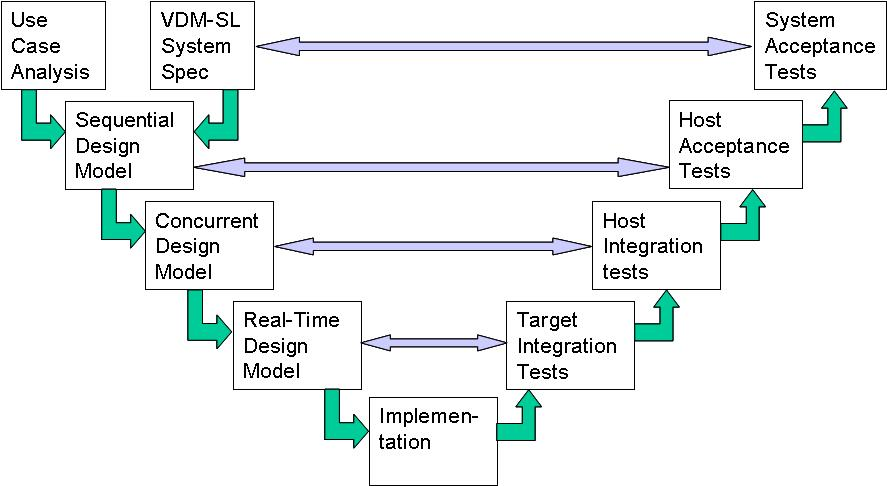
\includegraphics[width=\textwidth]{figures/lifecycle.jpg}
\end{center}
%\begin{picture}(350,330)
%\put(0,270){\framebox(80,60){\parbox{2cm}{Sequential Model}}}
%\put(90,180){\framebox(80,60){\parbox{2cm}{Concurrent Model}}}
%\put(180,90){\framebox(80,60){\parbox{2cm}{Concurrent Real-Time Model}}}
%\put(270,0){\framebox(80,60){\parbox{2cm}{Implementation}}}

%\put(40,270){\line(0,-1){60}}
%\put(40,210){\vector(1,0){50}}

%\put(130,180){\line(0,-1){60}}
%\put(130,120){\vector(1,0){50}}

%\put(220,150){\line(0,1){60}}
%\put(220,210){\vector(-1,0){50}}

%\put(220,90){\line(0,-1){60}}
%\put(220,30){\vector(1,0){50}}


%\end{picture}
\caption{Overview of Development Process}\label{fig:processoverview}
\end{figure}

In Figure~\ref{fig:processoverview} an overview of the different
phases we touch upon in this chapter is presented. This is the
traditional V-life cycle used by many industrial organizations as
an approximation of what goes on in reality (with iterations and feedback
between phases).  This
structuring in phases may be used either with a traditional waterfall
process model or for each iteration using Boehm's spiral model
\cite{Sommerville82, Boehm88}.  The difference is mainly that in the
spiral process model the artifacts with the highest risk will be
analyzed first, and this would have the consequence that in the
process we describe below one would abstract away from parts which
does not have any impact on the analysis needed to mitigate the
highest risks. The green arrows in the figure indicate the primary flow of 
information (and in this case VDM models) whereas the purple (vertical) lines
indicate that the tests conducted at the development phases (using models)
may be reused at the corresponding acceptance test level.

The development process will normally begin with analyzing the
informal requirements and capturing these to form a design-independent
specification of the system to be developed. Based on this description
one needs to structure the system into a static architecture and
create a sequential VDM++ design model of the system. This model would
then be extended to become a concurrent VDM++ design model. The
concurrent design model itself is then extended with real-time
information. At this stage it may prove necessary to revisit the
concurrent design model, as it may be that design decisions made at
that stage prove to be infeasible when real-time information is added
to the model (for instance, the model may not be able to meet its
deadlines). From the concurrent and distributed real-time VDM-RT design
model an implementation may be developed.  Testing of the final
implementation (and the different design-oriented models) may be able
to use the most abstract model as a test oracle. We return to the
different test phases in Section~\ref{sec:tests}.

When developing a model of a real-time system, it is typically
difficult to separate the system from the environment in which it is
executing, and with which it interacts.  Therefore it is often the
case that all the relevant parts of the environment are also modelled.

\section{Requirements Capture}

The first phase of a system development process is to capture the
requirements of the new system. This phase is also called the system
analysis phase or the specification phase depending upon the different
company standards. We recommend that this stage be performed in either
UML or by using VDM-SL. For both approaches, the starting point is the
informal requirements, and the end point is a specification of the
requirements to the system, which is independent of any design
concerns, as shown in Figure~\ref{fig:inputoutput}. In the Model
Driven Architecture (MDA) \cite{MDA} terminology this is called a
Platform Independent Model (PIM).

\begin{figure}
\begin{center}
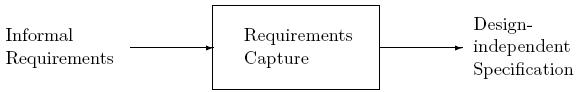
\includegraphics[width=0.8\textwidth]{figures/reqcapture.jpg}
\end{center}
\caption{Overview of the input/output relationship for requirements capture}\label{fig:inputoutput}
\end{figure}

\begin{figure}
\begin{center}
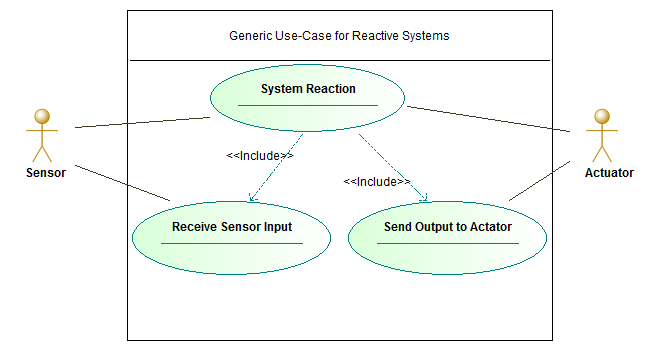
\includegraphics[width=0.8\textwidth]{figures/generalusecase.png}
\end{center}
\caption{General use case for embedded systems}\label{fig:usecase}
\end{figure}

Both approaches are described in the sequel. In
Section~\ref{subsec:capuse} a conventional UML \cite{UML20} approach
is described, in which use-cases are created and discussed with
clients and users. This approach is illustrated with the counter
measures example in Section~\ref{sec:usecase}.

Alternatively a flat VDM-SL model, and a Graphical User Interface
(GUI) connected to this model to allow users and clients to interact
with the animated model could be created (in a similar manner to that
described in \cite{CashPoint}). This approach is described in
Section~\ref{subsec:VDMSL} and illustrated with the counter measures
example in Section~\ref{sec:VDMSL}.

\subsection{Capturing Requirements with UML Use Cases}\label{subsec:capuse}

In this Section it is described how requirements may be captured using
UML use case diagrams \cite{UML20}. The presentation assumes that the
tool Rational Rose \cite{Rose&00} or the tool Enterprice Architect 
is used, but other UML tools have
similar functionality. An example of this analysis is given in
Section~\ref{sec:VDMSL}

\subsubsection{Find the actors and use cases}

\begin{itemize}
\item Identify the frontiers of the system and their principal functionality.
\item Identify the actors in the system. The actors may be equipment,
users or the system environment.
\item Identify use cases.
\item Summarize the role of each actor and the goal of each use case.
\item Arrange the actors and use cases into related packages.
\item Describe the use cases using use case diagrams (in
Figure~\ref{fig:usecase} such an example is shown).
\item Describe the states of the system using a state transition diagram.
\end{itemize}

\subsubsection{Structure the use case model}

\begin{itemize}
\item Define the relation {\tt <<includes>>} between use cases
(e.g.\ in Figure~\ref{fig:usecase}).
\item Define the relation {\tt <<extend>>} between use cases.
\item Define the generalization relation between use cases.
\item Define the generalization relation between actors.
\end{itemize}

These stereotypes are defined in the UML 2.0 standard \cite{UML20}.

\begin{figure}
\begin{center}
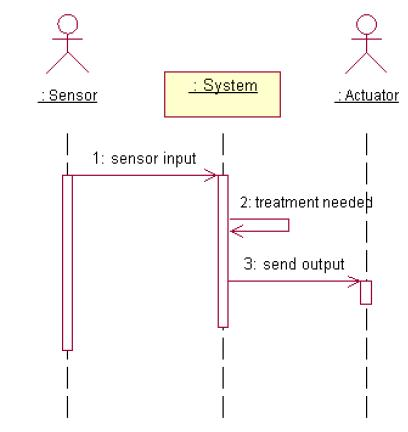
\includegraphics[width=0.5\textwidth]{figures/generalseqdia2.jpg}
\end{center}
\caption{General Sequence Diagram for an Embedded System}\label{fig:seqdiag}
\end{figure}

\begin{figure}
\begin{center}
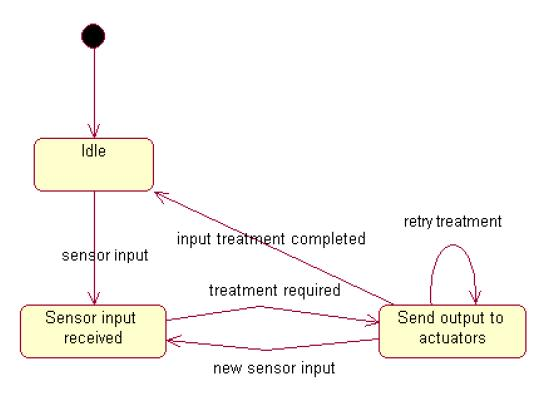
\includegraphics[width=0.8\textwidth]{figures/generalstatedia.jpg}
\end{center}
\caption{General Activity Diagram for an Embedded System}\label{fig:activitydiag}
\end{figure}


\subsubsection{Specify the use cases in detail}

For each use case

\begin{itemize}
\item Detail the interaction between the actors and the system.
\item Structure the interactions between the actors and the
system. Note that normal sequences of actions should be distinguished
from abnormal sequences of actions (e.g.\ exceptional cases, degraded
cases, failure cases etc).
\item A use case could perhaps be associated with a user interface
that is already defined. This aspect should not be developed with
particular concern to the human-computer interface, but it is useful
to represent this interface with the description facilities of the use
case.
\item If useful, all the exit scenarios of a use case can be
specified. The difference between a use case and an associated
scenario is that a scenario is an instance of a use case.
\item Illustrate each use case or scenario:
\begin{description}
\item[Using a sequence diagram:] At this stage the system in question
is not yet divided into classes so such sequence diagrams will only
show the flow of control between the actors and the system. In version
2.0 of UML there are also possibilities to include information about
alternative flow of control primitives \cite{UML20}. Typically a
diagram should fit on one sheet of A4/letter paper. An example of this
is shown in Figure~\ref{fig:seqdiag}.
\item[Using a collaboration diagram] as an alternative view of the
sequence diagram. This allows representation of a simple scenario.
\item[Using an activity diagram] if necessary (or multiple activity
diagrams). An example of this is shown in
Figure~\ref{fig:activitydiag}.
\item[Using a state diagram] if the complexity of the use case
justifies it.
\end{description}
\end{itemize}

\subsection{Capturing Requirements Using VDM-SL}\label{subsec:captureVDM}
\label{subsec:VDMSL}

As an alternative to the use case approach described above in
Section~\ref{subsec:capuse}, the informal requirements can be captured
in a design-independent way using VDM-SL. In the first instance this
follows Chapter 2 of \cite{Fitzgerald&98b,Fitzgerald&05,Fitzgerald&09}. At this
stage, time can be included as a state variable and can be driven as
part of the model. In this way the functional, timing, and
time-dependent functional requirements can be captured within one
model.

The general strategy used to model a real-time system is to model the
system as one top-level operation where the input is considered as a
sequence of events which comes into the system to be modelled. The
output from the top-level operation will then be those events which
are sent out from the system. If time is essential, all input and
output events must be tagged with the time at which the event appeared
(i.e.\ an extra field in the event record values). In this way time is
modelled explicitly in such a VDM-SL model.

The general structure of the top-level function in such a VDM-SL model
would look like (this is without taking the closed loop complications
into account at the top-level):

\begin{lstlisting}
operations

  PerformSystemReaction: seq of SensorInput ==> 
                         seq of ActuatorCommand
  PerformSystemReaction(inputseq) ==
   if inputseq = []
   then []
   else SensorTreatment(hd inputseq) ^ 
        PerformSystemReaction(tl inputseq)
\end{lstlisting}

The types \texttt{SensorInput} and \texttt{ActuatorCommand} can then
either include the time explicitly as an attribute or a fixed
stepping length between the inputs can be modelled such that the time
is represented implicitly. When the treatment of a sensor input may
take longer than the next sensor input arrives, it is likely that this
will cause an interruption of the existing treatment. In that case the
functional description using the functions \texttt{SensorTreatment} and
\texttt{Perform\-System\-Reaction} used above are more complicated. A full example
of such a VDM-SL model is given in Section~\ref{sec:VDMSL}. Naturally
the feedback loop where the way the environment behaves depending upon
the system reaction cannot be taken appropriately into account with
this approach. Thus, if a sequence of sensor input does not fit with
the order of the system output sequence. It simply means that the
given input sequence does not match reality. Despite this such a high
level executable model may be valuable to act as an oracle against
real final implementation scenarios.

In order to accomodate for a proper feedback loop one simply needs to
introduce an accumulating parameter with the actuator commands to be 
issued unless new sensor inputs are detected. That accumulating
parameter can then be manipulated accordingly when new sensor
input arrives. This approach is actually followed in 
Section~\ref{sec:VDMSL}.

Note that it is possible to construct a GUI to animate the VDM-SL
model to allow users, domain experts and clients to see how the
requirements have been captured.  This animation technique allows
visualization of a number of scenarios where the input/output
relations can be inspected.

\subsection{Validating Requirements Capturing}

Traditionally in the life-cycle only test planning would take place in
the early phases of a systems development \cite{Sommerville82}. One of
the advantages of the development process described here is, that it
makes it possible to carry out systematic testing, and thus get
feedback on such test plans, much earlier in the life cycle. If the
flat VDM-SL approach has been used for capturing the requirements,
then the GUI used for interaction with the client and users should be
reused, and the model should be animated to the satisfaction of the
client and users. At the final acceptance test of the completed system
the regression test environment should be reused as much as possible
by changing the script from execution of the abstract VDM-SL model to
execution of the final implemented system as a kind of proof of concept 
prototype.

\subsection{Criteria for Completion}

This stage is complete when:

\begin{enumerate}
\item The architecturally significant use cases have been completed 
      and they have been manually validation for example using inspection or
\item The abstract VDM-SL model has been completed and validated.
\end{enumerate}

\section{Sequential Design Model}

A sequential design model must describe both the data that is to be
computed, and how it is to be structured into static classes, without
making any commitment to a specific dynamic architecture.

The first stage in creating a sequential model is to decide on a
static architecture. A static architecture is an arrangement of system
behaviour into classes/objects. There already exist a number of
classical books about deriving a class structure
\cite{Rumbaugh&91,Meyer88,Booch&97,Douglass99} so we will not include that
discussion in this document. This document will only provide a few
guidelines about how the classes can be identified and discuss to what
extent a VDM-SL model can be reused when one produces VDM++ skeletons
for each of the identified classes in a system.

The approach to developing a static architecture depends on whether
the UML approach or the VDM-SL approach was used to capture
requirements. These are therefore treated separately below. Note
that whichever requirements capture approach was used, the result of
the current phase will always be VDM++ class skeletons.

\subsection{If UML Was Used For Requirements Capture}\label{subsec:UMLreq}

If UML was used for requirements capture, the uses cases are analyzed
to identify a number of classes, and from these classes VDM++ class
skeletons are produced.

\subsubsection{Identify the classes}

This activity consists of identifying concepts, and more generally,
abstractions from the specification resulting from the requirements
capturing process. Also, relationships between these classes should be
defined. Entire books are written about this subject so here only a
short introduction is provided using terminology from the literature
\cite{Kruchten00}. Note that at this stage it is more important to identify the
classes, than to add detail to particular classes. There should be
classes both for the system itself and also for the artifacts from the
environment in order to be able to capture the feedback from the
environment. However it may be possible to define some attributes and
relations on the basis of dependencies identified by use cases. From
these classes, a first class diagram may be created.

\begin{figure}
\begin{center}
\begin{tabular}{|l|l|l|l|l|}\hline
         & Actor & Entity Class & Boundary Class &
           Control Class \\ \hline
Actor                        &   N/A  & No & Yes & No \\ \hline
Entity Class &  No    &No\footnotemark & No & Yes \\ \hline
Boundary Class& Yes   & No & No  & Yes \\ \hline
Control Class & No    &Yes & Yes & Yes \\ \hline
\end{tabular}
\end{center}
\caption{Recommendations for Associations Between Classes\label{tab:assoc}}
\end{figure}
\footnotetext{Unless there exists an aggregation or composition between the two classes.}

The following stereotypes should be used for each class:
\begin{description}
\item[Entity Class] Indicates that the class contains
persistent data.
\item[Control Class] Indicates that the class controls, sequences and coordinates activity in the system.
\item[Boundary Class] Indicates that the class is an
interface to an actor (a part of the environment to the system).
\end{description}

A number of recommendations apply to the use of associations between
classes. These can be found in Table~\ref{tab:assoc} where ``No''
indicates that they should not be combined and ``Yes'' indicates that
they can be combined.

\subsubsection{Producing VDM++ Class skeletons}\label{subsub:skeleton}

When the definition of classes is finished, the next stage is to
generate skeleton VDM++ classes for the model. Class skeletons can
automatically be generated using UML class diagrams and the UML-VDM++
link feature from \vdmtools\ or the Overture linkage to Modelio. 
%This automatically generates a
%file for each class in the Rose repository, in Microsoft Word RTF
%format. 
Each such file contains the VDM++ skeleton of the class. 
%From
%now on it is possible to adjust both the VDM++ model in the Microsoft
%Word files and the Rational Rose model. The Rose-VDM++ link is able to
%merge such changes.

\subsection{When VDM-SL was used for Requirements Capturing}

When the informal requirements are captured in a precise way using
VDM-SL it is often possible to conceptually
reuse most of the VDM-SL operations
inside the VDM++ classes where structuring and design decisions are taken
into account.  However, for
real-time systems the nature of the VDM-SL model will traditionally be
very different from the design which is needed in the system
architecture so less reuse should be expected for this kind of
systems. Still, the use of VDM-SL for requirements capturing may
still be valuable for such systems.

Having defined the formal functional requirements in the VDM-SL model,
these requirements should be mapped to a static architecture. That is,
skeleton VDM++ classes should by synthesized from the VDM-SL
model. This is not an automatic process and we do not claim to be
original or better than anybody else with guidelines about how one
most conveniently divides the system into components or classes.  The
following guidelines should be used during this synthesis:

\begin{itemize}
\item Record types in the VDM-SL model typically become classes in the
static architecture.
\item Activities which are functionally independent will typically be
encapsulated in separate classes in the static architecture.
\end{itemize}

A guideline which is always good to follow to divide into classes and
relationships between classes, is that one should model both the
system in question and its environment. Typically each sensor and
actuator will get their own classes. From a deployment perspective
instances of such classes will also typically be allocated to their
own \texttt{CPU}'s. These would be the actors from the use case
diagram. Traditionally it is often a good idea to have a
\texttt{World} class which controls the overall interaction between the
environment and the classes representing the system in question. This
class can then be used for setting up the appropriate connections
between the different objects and testing the interaction between
them.

An example of synthesizing such class skeletons is given in
Section~\ref{sec:skeleton}.

\subsection{Class Descriptions in VDM++}

Class skeletons should evolve into complete specifications. This
involves completing operation bodies for those operations already
referred to in the previous stages, and adding any auxiliary functions
and operations.

Where possible invariants on types and instance variables should be
identified and specified. Pre-conditions should be specified for all
operations and functions that are non-total, and post-conditions
should be specified wherever it is meaningful to do so (i.e.\ where it
does not lead to restatement of the function or operation body, if
present).

An example of completed class descriptions in VDM++ is given in
Section~\ref{sec:sequential}.

\subsection{Modelling of the Environment}

It is often difficult to model the behaviour of a reactive real-time
system without reference to the environment in which it is
executed. Thus it is often convenient and useful to create classes
(and/or threads in a concurrent model) which represent this
environment. These classes may then be used to inhabit the model with
test data.

\subsection{Typical Design Structure}\label{sec:typicalclassdiag}

\begin{figure}
\begin{center}
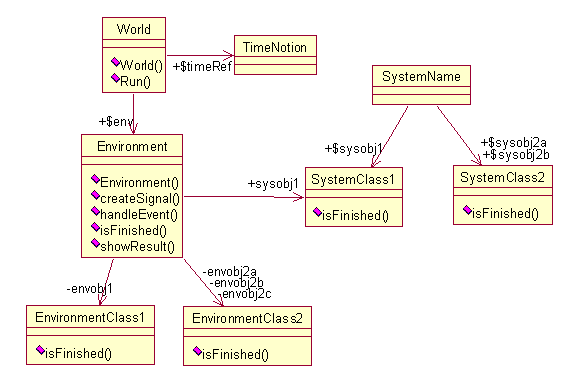
\includegraphics[width=0.8\textwidth]{figures/generalclassdiag.png}
\end{center}
\caption{General Class Diagram for an Embedded System}\label{fig:classdiag}
\end{figure}

Figure~\ref{fig:classdiag} illustrates the general static class structure 
recommended for reactive embedded systems in the guidelines in this document.
It is recommended to always have a class responsible for the 
\texttt{Environment} and a class responsible for the composition of the
components using inside the system called \texttt{SystemName}. It is also
recommended always to have a class called \texttt{World} that contain 
a constructor responsible for setting up both the environment and the 
system components enabling them to carry out a scenario. 

The scenario is
then usually invoked by an operation called \texttt{Run}. Thus, typically
one can made a call like \texttt{new World().Run()} where the details
of the scenario are either given as a parameter or stored in a file that
will be read by the standard \texttt{IO} class. Since reactive systems 
will react to stimuli from the environment \texttt{IO} is typically used 
inside the \texttt{Environment} class or one of the other classes 
representing parts of the environment (\texttt{EnvironmentClass1} and 
\texttt{EnvironmentClass2} in Figure~\ref{fig:classdiag}).

In addition to a constructor the \texttt{Environment} is recommended to 
contain operations to provide input for the system (\texttt{createSignal})
and operations to receive feedback from the system (\texttt{handleEvent}). 
It is also recommended to provide an operation called \texttt{isFinished}
for all classes that play an active role in a scenario (this operation shall
indicate when the processing is finished locally). This holds for
both environment and system classes. As will be clear after the  
example is presented in Chapter~\ref{chap:example} the signature for 
\texttt{isFinished} will in the sequential model typically yield a Boolean
result, but that will change in the concurrent and distributed models.
For the \texttt{Environment} class 
it is also necessary to provide some kind of operation that can show the
result of running a given scenario (\texttt{showResult}).

It is recommended to use static public instances from the \texttt{World}
and the overall system class \texttt{SystemName} in order for them to be 
accessible throughout the model without having to pass the object references
around. This also includes some kind of notion of time if time is of 
importance for the reactive system (which it usually is). In the sequential
model it is recommend to use a basic \texttt{Timer} class here, but in the 
concurrent model a stronger notion of time and synchronisation as will be seen
in Section~\ref{sec:designconcur}.

Finally it is worth mentioning that it is recommended to let the flow of
control be steered from the \texttt{Environment}. At the sequential level
this is typically done using a loop until both the environment and the
system are finished (using different \texttt{isFinished} operations. Inside 
the loop \texttt{Step} operations are used for stepping over time and 
passing the control around to the different components of the system.

\subsection{Validation of the Model}

Whenever possible the model should be executed to allow validation. If
the use cases approach has been used in the requirement capturing
process, then execution should ensure that model execution satisfies
all of the use cases identified.

Note that even if the whole model is not executable, portions of it
may be, and therefore these portions should be validated in the manner
described above.

In addition to the animation technique for validation of the model
described above a more systematic traditional testing approach should
also be used to validate the model.  Thus, test cases should be
defined and an automatic test script should be made such that the test
cases can be used in a regression fashion during this phase and reused
in subsequent phases. The VDMUnit test framework from
\cite{Fitzgerald&05} (chapter~9) may be used with advantage here (include the 
\texttt{VDMUnit} standard library).

\subsection{Criteria for Completion}

This stage is complete when:

\begin{enumerate}
\item The VDM++ model is syntax and type correct;
\item The UML class diagram and VDM++ model are synchronized;
\item The model has been validated;
\item XX\%\ test coverage for executable portions of the model
(uncovered parts should be justified).
\end{enumerate}

Here ``XX'' is a figure that would be determined by the standards used
by each individual company or organization.

\section{Concurrent VDM++ Design Model}\label{sec:concur}

The objective in developing a concurrent VDM++ design model is to take
the first steps towards a particular dynamic architecture, without
worrying in the first instance about real-time behaviour. An example
of such a model is given in Section~\ref{sec:concurmod}.

\subsection{Identification of Threads}

The first step in developing a concurrent model is to identify which
computations can be performed independently of each other. These
computations may then be separated into independent threads. Often,
this separation will be forced by hardware constraints and/or
pre-defined architectural requirements. While it is worthwhile
identifying as many independent threads as possible, in general the
number of threads in the system should be minimized. This is because
(again in general) threads increase complexity of the model and make model
validation more difficult.

\subsection{Communication}

After identification of threads, it must be decided which threads
communicate with each other, and what values are passed. Accordingly
object sharing between threads should be specified. For classes
representing shared objects, appropriate synchronization should be
specified.

\subsection{Synchronization Points}

In addition to synchronized object sharing it may be necessary to
introduce explicit synchronization points. That is, ensure that a
particular thread does not proceed beyond a specified point, until
another thread has reached an appropriate state. This can be important
to ensure correct sequencing amongst the different threads, or else to
ensure freshness of data. In general if an operation both reads from
and writes to instance variables it will be advantagous to make it
mutexed with itself.

\subsection{Validation of the Model}

The model should be executed using the same scheduling policy as that
used by the target real-time kernels used for the processors in the
target environment. Upon execution the model should be free of
deadlocks (note that there is not yet a formal analysis conducted in 
Overture for this, so it is limited to the scenarios used as test
cases). Moreover the model should functionally yield the same
results as the sequential model, perhaps modulo some adjustments with
the formulation of the values and the time at which they appear.

\subsection{Typical Design Structure}\label{sec:designconcur}

The general structure from Figure~\ref{fig:classdiag} is also recommended 
for concurrent models. The main changes from the sequential model are:

\begin{itemize}
\item Flow of control is changed such that instead of it residing with the
      \texttt{Environment} it will be distributed to all the active parties
      and thus the body of the \texttt{Step} operations are typically 
      turned into threads. 
\item Synchronization between the different threads are specified using
      permission predicates and mutex constraints.
\item The signature for the \texttt{isFinished} operations is changed 
      such that no value is returned. Instead the Boolean expression is 
      typically used as permission predicates. This is a way to block
      the threads requesting this operation until the corresponding 
      instance indeed is finished with its business.
\item It is recommended to replace the simple \texttt{Timer} class with
      a \texttt{BaseThread} and a \texttt{TimeStamp}
      class from Appendix~\ref{sec:TimeStamp} in order
      to easily synchronize the steps taken now when the flow of control
      is distributed to multiple threads.
\end{itemize}

\subsection{Criteria for Completion}

\begin{enumerate}
\item The VDM++ model is syntax and type correct.
\item The UML class diagram and VDM++ model are synchronized.
\item The model has been validated.
\item The model displays no deadlocks;
\item XX\%\ test coverage for executable portions of the model
(uncovered parts should be justified).
\end{enumerate}

Here ``XX'' is a figure that would be determined by the standards used
by each individual company or organization.

\section{Concurrent Real-Time and Distributed VDM-RT Design Model}

At this stage real-time information is added to the model. In addition
if the system in question is to be distributed over multiple
processors allocation of functionality to such processors are
conducted. The timing analysis described in
Section~\ref{sec:timingintro} is then performed. Following such
analysis, it may be concluded that the proposed dynamic architecture
is in fact infeasible. Therefore it might be necessary to revisit
Section~\ref{sec:concur} and revise the dynamic architecture or revise
the deployment of the functionality to \texttt{CPU}'s or 
their capabilities. An
example of a concurrent real-time model is given in
Section~\ref{sec:realtime}.

%\subsection{Default Duration Information}

%If the target processors are not one of the standard ones (currently
%the Motorola 68040 is the only supported processor), then a file
%containing default duration information should be defined for the
%necessary target processors. In principle this is straightforward to
%define, based on the data book for that processor. However, with
%modern processors using caching or a pipeline architecture it may be
%more difficult to be able to achieve precise estimates because the
%time for different basic instructions depends upon the instruction
%context, and that is impossible to take into account with this
%framework.

\subsection{Duration and Cycle Statements}

For those parts of the model where knowledge of real-time behaviour
exists (e.g.\ components which are being reused) duration statements
should be used to give precise estimates of fixed execution times. The 
cycle statements should be used to give precise estimates of the 
execution time relative to a processor (in the form of the number of 
expected clock cycles).

For those parts of the model which are effectively modelling the
environment. Depending upon the accuracy needed for the VDM-RT model of
the system under design the model of the environment should be more
elaborate. Here is is possible to have different instances in the
environment on each their own virtual processor or even be modelled
using its own formalism and validated using a co-simulation
interface. 
However, it is also
possible for example to model the environment to constrain the
environment instances to be deployed on the same processor.

For modelling closed loop systems, a duration statement should be used
to force a delay in the time between sending a command to an actuator,
and seeing its effect at a sensor.

\subsection{Task Switching Overhead}

The task switching overhead for the target real-time kernel should be
ascertained. This value should be used as the task switching overhead
in Overture and \vdmtools\ during execution of the model.

\subsection{Typical Design Structure}\label{sec:designvice}

The general structure from Figure~\ref{fig:classdiag} is still recommended 
for the real-time distributed models. The main changes from the concurrent
model are:

\begin{itemize}
\item The \texttt{SystemName} class is now changed to become a
  {\bf\ttfamily{system}} 
      where additional instance variables are introduced for all the
      \texttt{CPU}'s and \texttt{BUS}'es that one would like to distribute
      the functionality to. In addition a constructor is introduced here
      where the actual deployment of the static instance variables to
      \texttt{CPU}'s take place. In addition it is possible to define the
      priority of different operations in this constructor in case 
      priority-based scheduling is used on some of the \texttt{CPU}'s. 
\item Optionally a system can be created of the \texttt{Environment} class
      as well. In case this is not done \vdmtools\ will simply execute
      all functionality on a virtual \texttt{CPU} for each instance created in the
      \texttt{World} class. Thus, it may be valuable making a system for
      the \texttt{Environment} in case that it is essential that the 
      environment functionality have dependencies upon each other and thus
      when one instance is executing another instance cannot also be 
      executing in a true parallel fashion.  
\item A number of the operations that simply need to start execution on
      a different thread are made asynchronous using the {\bf\ttfamily{async}}
      keyword. Note that in essence if such two instances are deployed at 
      different \texttt{CPU}'s behind the back of the user they will
      communicate over a \texttt{BUS} and here the notion of synchronism
      is essential.
\item Some of the threads (typically those that previously had \texttt{Step}
      functionality) are turned into periodic threads.
\item The explicit notion of time (at the concurrent level using the 
      \texttt{BaseThread} and \texttt{TimeStamp} classes) is removed. 
      Now time is implicit and it
      is possible to make use of the keyword {\bf\ttfamily{time}} to refer to the
      current time on a given \texttt{CPU}.
\end{itemize}

\subsection{Validation of the Model}

The model should be executed using as many different scenarios as are
necessary to satisfy the following two criteria:

\begin{enumerate}
\item To achieve the required test coverage as dictated by the
completion criteria for this stage;
\item To cover all use cases identified during requirements capture
(if the UML was used to capture the requirements).
\end{enumerate}

This execution can be used to check correctness of computed values in
these scenarios, and the absence of deadlocks. Note that introduction
of real-time information could in itself introduce deadlocks to the
model, as it could cause the scheduler to make different decisions to
those made during execution of the untimed model.

\subsection{Timing Analysis}

Execution of the model will create a time trace file which
may be analyzed subsequently (examples of this are shown in
Chapter~\ref{chap:timetrace}). Analysis should establish the
following:

\begin{itemize}
\item No periodic threads miss their deadlines.
\item All real-time response requirements are satisfied (all hard 
      real-time deadlines are met with the used scenarios).
\end{itemize}

Here the \showtrace\ feature from Overture is particular valuable 
in the automatic analysis of these timed traces. It is able to automatically
to provide:
\begin{itemize}
\item A graphical overview of the physical architecture with the \texttt{CPU}'s
      and the \texttt{BUS}'es.
\item Show an overview of the overall execution and communication between
      the \texttt{CPU}'s.
\item Show a detailed overview of the instances and the execution and 
      communication between these at a single \texttt{CPU} in a detailed
      fashion.
\end{itemize}

\subsection{Criteria for Completion}

\begin{enumerate}
\item The model is syntax and type correct.
\item The UML class diagram and VDM-RT model are synchronized.
\item The model is schedulable.
\item The model displays no deadlocks.
\item The model is functionally correct for all executed scenarios.
\item The model includes a deployment of functionality to a physical
      architecture.
\item All periodic threads make their deadlines with the chosen physical
      architecture for the tests conducted.
\item Any real-time response requirements are satisfied for the tests
conducted.
\item XX\%\ test coverage for executable portions of the model
(uncovered parts should be justified).
\end{enumerate}

Here ``XX'' is a figure that would be determined by the standards used
by each individual company or organization.

\section{Implementation}

The approach to implementation depends upon the target implementation
language and constraints on program structure and performance. If C++
is the implementation language, and dynamic memory allocation is
permitted, then use of the \VDMTools\ C++ Code Generator is possible. This
implies a massive reduction in effort, since the implementation is
obtained by one mouse click. Similarly if Java is the implementation
language, the \VDMTools\ Java Code Generator can be used. However, such
automation should not be relied upon for hard-real-time systems and
the distribution of the model os {\bf not} taken into account in this
code generation.

In other circumstances the implementation must be written by
hand. However this tends to be quite straightforward due to the
quantity and depth of information acquired during the modelling
stages. Typically a number of rules can be applied reasonably
mechanically, to translate the VDM-RT model into code. 
%For instance
%\cite{Bousquet00} gives a list of rules that can be applied to translate
%VDM++ models into an Ada 95 implementation.

\section{The Different Test Phases}\label{sec:tests}

As identified in Figure~\ref{fig:processoverview} there are a number
of different phases with different levels of testing conducted on the
system being developed. With conventional development technology it is
normally not possible to validate whether a system under development
will be able to meet its deadlines before the target integration test
phase. If these tests show that it is not possible to meet the
deadlines, there is therefore a significant cost involved in
redesigning the system and its corresponding implementation to improve
this situation. The approach described in this document aims to find
potential bottlenecks in the system even before the final
implementation is made. The aim is to be able to sit on the host
computer (where the development takes place) and simulate the timing
behaviour of the concurrent real-time VDM-RT design model with
information about the timing behaviour of the intended possibly
distributed hardware platform.

\begin{figure}
\begin{center}
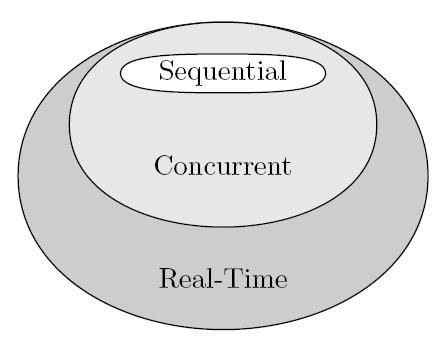
\includegraphics[width=0.5\textwidth]{figures/VDM++levelsofmodels.jpg}
\end{center}
\caption{Relationship Between VDM Models}\label{fig:relationship}
\end{figure}

With the approach described in this document the test cases used in
the different test phases are already executed when the design is made
and then reused with the final implementation subsequently. This is a
major change compared to the conventional way of development where
feedback about the timing properties of a particular design only comes
very late in the development process. Note however that each of the different
models gets closer and closer to reality, where the most abstract models
have a somewhat idealised view of the system and its environment, the later
models takes more and more details into account.

\section{Discussion}

In this chapter we have described the evolution of one VDM-SL model
and three object oriented VDM models: a sequential model, a concurrent
model and a concurrent distributed real-time model. There is no formal
relationship between them in the sense that no formal relationship has
been established between any of the models. This is consistent with
the pragmatic software engineering approach advocated in this process,
in contrast to a pure formal development. Nonetheless, since the
process involves adding detail to each model, to obtain the next
model, in some sense we can consider each model a sub-model of the
next, as shown in Figure~\ref{fig:relationship}.  That is to say, the
concurrent model is an extension of the sequential one, and the
real-time and distributed model is an extension of the concurrent
one. Each of the models get more and more concrete and complex, but
gradually closer and closer to reality.

\chapter{Example Development}\label{chap:example}

In this chapter an example development process is presented. This
development goes through each of the steps from
Chapter~\ref{chap:process}. The system developed is a simplified
version of an actual real-time system. The chapter begins by
presenting the informal requirements for the system and then the
different models developed are presented.

\section{The Counter Measures System}\label{sec:CMdesc}

The application to be modelled in VDM is the controller for a
missile counter measures system. This takes information from sensors
concerning threats and sends commands to hardware which releases
flares intended to distract the threat sensed.  The overall high-level
architecture is shown in Figure~\ref{fig:contextdiag}.

Flares are released in a timed sequence, the number of flares released
and the delay between releases depending on the threat and its angle
of incidence with the missile. Different places around an aircraft
different flare dispensers or magazines are located dealing with
threats arriving from different angles. The threat sensors relay the
ID of the threat to the controller. For each different kind of ID and
the angle of the missile the controller must then derive a plan for
how to deal with the given threat by firing a sequence of flares with
a given pattern with a given flare dispenser (a magazine) dealing with
the given angle. Such a pattern contains the number of flares to be
fired and the delay between each firing. The task communicates the
stated number of firings to the flare release hardware with the
specified delay between each communication. For the purposes of this
document it is assumed that there are only two kinds of physical
flares.

\begin{figure}
\begin{center}

\includegraphics[width=\textwidth]{figures/contextdia.jpg}
\end{center}
\caption{Context Diagram for the Counter Measures System}\label{fig:contextdiag}\end{figure}

\begin{figure}
\begin{center}
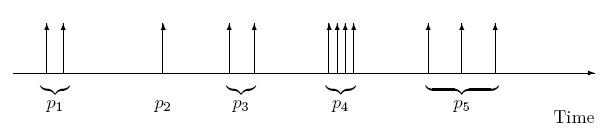
\includegraphics[width=\textwidth]{figures/flareseqs.jpg}
\end{center}
\caption{Example Firing Sequence}\label{fig:firing}
\end{figure}


An example firing sequence is shown in Figure~\ref{fig:firing}. Flare
release commands are represented by the vertical arrows. Five actions
are depicted in this figure. For simplicity we will assume that only
three kinds of missiles are known to the system: A, B and C where they
have increasing priority in this order. Similarly we simplify the
example by supposing that there are only two kinds of physicals
flares, together with the special ``Do Nothing'' flare, which requires
that nothing is released for a specified duration.  For the purposes
of this example we assume the counter measures system for each flare
dispenser to respond to the different missile types as shown by the
firing sequences in Figure~\ref{fig:missileresp}.

The following requirements apply to this system:

\begin{enumerate}
\item If while computing the firing sequence with a flare dispenser 
for a given threat from an angle treated by the same flare dispenser,
another threat is sensed (in the same angle area), 
the system should check the priority of the
more recent threat and, if greater than the previous one, should abort
computation of the current firing sequence.  Computation of the new
firing sequence should then take place.
\item If different threats are sensed with angles that are treated by 
different flare dispensers the corresponding firing sequences shall be 
performed in parallel.
\item The controller should be capable of sending the first flare
release command within 250 milliseconds of receiving threat
information from the sensor.\label{timereq34}
\item The controller should be able to abort a firing sequence within
130 milliseconds.
\end{enumerate}

The system to be developed can be composed of a number of different
hardware components (sensors and flare dispensers) organised in a
physical architecture to be determined.

\section{UML Use Cases for Requirements Capture}\label{sec:UMLreq} 
\label{sec:usecase}

If use cases are used for capturing the requirements for the counter
measures system we produce a use case diagram like the one shown in
Figure~\ref{fig:counteruse}. For each of the ovals (the graphical
representation of a use case) a textual description of the use case
must be made. This is typically done in an itemized fashion. In the
three subsections below we show such a description for each of the
different use cases.

\begin{figure}
\begin{center}
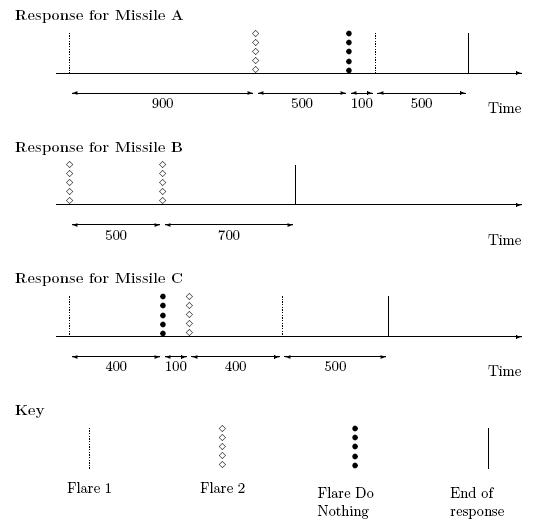
\includegraphics[width=\textwidth]{figures/responses.jpg}
\end{center}
\caption{Example Missile Responses Used in the Models\label{fig:missileresp}}
\end{figure}

\begin{figure}
\begin{center}
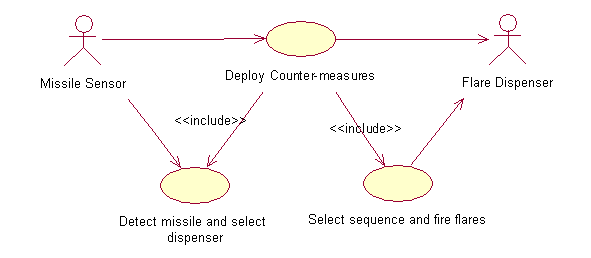
\includegraphics[width=\textwidth]{figures/CMusecases.png}
\end{center}
\caption{Use Case Diagram for the Counter Measures System\label{fig:counteruse}}\end{figure}

\subsection{Deploy Counter-measures}

\begin{description}
\item[Primary Actor(s):] Missile Sensor and Flare Dispenser
\item[Secondary Actor(s):] None
\item[Intent:] This use case is responsible for taking the given
threat identification and fire flares accordingly.
\item[Assumptions:] All potential threats are identified.
\item[Known Limitations:] If threats come too close to each other the
system may not be able to manage to deal with all of them.
\item[Includes:] ``Detect Missile and Select Dispenser'' and ``Select Sequence
and Fire Flares''
\item[Pre-conditions:] A threat has arrived and has been detected by
a missile sensor.
\item[Course of action:] When a new threatening missile has been
detected by a missile sensor the appropriate flare dispenser should be
determined upon the angle of attack. Then, it should be determined if
another threat is already being handled by the flare dispenser. In
that case the priority of the thread identification must be compared
and if the new threat has a higher priority its sequence of flares
must be determined and that flare dispenser must interrupt what it is
currently doing and start firing this new sequence. If the priority is
equal to or lower the threat is simply ignored. If no threats have
been detected previously the corresponding sequence of flares must be
determined and subsequently fired using that flare dispenser. This is
illustrated in the state diagram shown in
Figure~\ref{fig:counterstate}.
\item[Post-conditions:] When the firing of the flares is complete the
threat should be distracted and no longer be targeting the system
guarded by the counter measures system.
\end{description}

\subsection{Detect Missile and Select Dispenser}

\begin{description}
\item[Primary Actor(s):] Missile Sensor
\item[Secondary Actor(s):] None
\item[Intent:] This use case is responsible for taking the given
threat identification and its angle of attack and based on this determine 
what flare dispenser to select.
\item[Assumptions:] All potential threats are identified.
\item[Known Limitations:] If threats come too close to each other the
system may not be able to manage to deal with all of them.
\item[Includes:] None.
\item[Pre-conditions:] A threat has arrived and been detected by the
missile sensor.
\item[Course of action:] Whenever a thread identification and its 
angle of attack is received
the responding flare dispenser must be selected and the sequence of 
flares fires must follow the identification from
Figure~\ref{fig:missileresp}.
\item[Post-conditions:] The correct flare dispenser and the flare sequence 
to be fired has been identified.
\end{description}

\subsection{Select Sequence and Fire Flares}

\begin{description}
\item[Primary Actor(s):] Flare Dispenser
\item[Secondary Actor(s):] None
\item[Intent:] This use case is responsible for performing the actual
firing of a sequence of flares according to the timing requirements
described in Section~\ref{sec:CMdesc}.
\item[Assumptions:] All potential threats are identified.
\item[Known Limitations:] There is probably a physical limit
concerning how close the different flares can be fired after each
other.
\item[Includes:] None
\item[Pre-conditions:] A sequence of flares have been identified.
\item[Course of action:] An internal timer is started and the
different flares are fired by the flare dispenser at the times
identified by the firing sequence.
\item[Post-conditions:] All necessary flares have been released.
\end{description}

\begin{figure}
\begin{center}
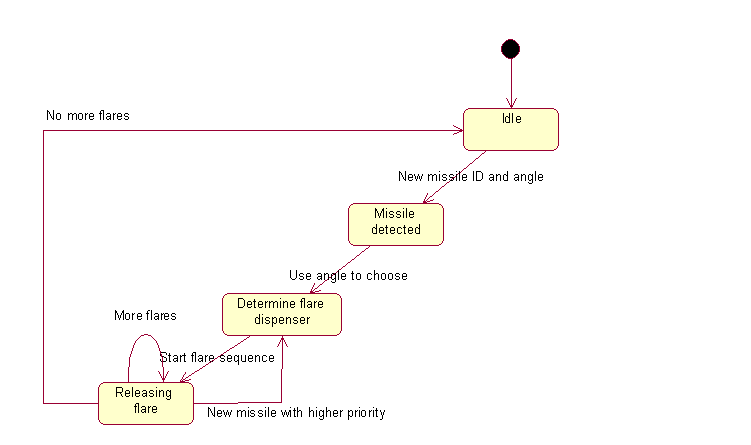
\includegraphics[width=\textwidth]{figures/CMstate.png}
\end{center}
\caption{State Diagram for Deploying Counter Measures\label{fig:counterstate}}
\end{figure}

\subsection{Summary}

As it can be seen from the use case descriptions given above the key
functionality of the counter measures system is identified by the use
cases. It is an abstract way of looking at the system, independent of
the different design issues which must be taken into account later in
the development process. The use cases can be a first way to
communicate that one has captured the essential usage of the system to
other domain experts. The use case diagram can be a nice way to get an
overview of how the different use cases hang together, in particular
when more complex systems are to be modelled.  However, any validation
of the use cases can only take place in the form of manual
reviews. There is no way in which any kind of automated validation can
be performed when we deal with natural language formulations like the
ones shown above.

\section{VDM-SL for Requirements Capture}\label{sec:VDMSLreq}\label{sec:VDMSL}

In this section the requirements to the counter measures system are
captured in a precise way using VDM-SL. The intention is to end up
with an abstract specification independent of any design issue. The
development of the model follows the general principles from
Section~\ref{subsec:UMLreq}. The underlying modelling decisions made
in this first model is to inspect the first missile and determine what
the appropriate response should be if that was the only threat received.
In case there are more than one missile arriving in an area before the 
processing of the current missile the response is altered in case the 
priority of the new missile is higher than the current one.

\subsection{Definition of Types}\label{subsec:generaltypes}

The counter measures system takes \texttt{MissileInput}'s as
input. This is a sequence of values of pairs of \texttt{MissileType} and
\texttt{Angle}. \texttt{MissileType}'s are
constant values representing the different possible missiles that
could be detected. In this case we have three different missiles, for
testing purposes, together with the special value \texttt{<None>}
representing the absence of any missile. \texttt{Angle} for simplicity 
is modelled as a number from 0 to 360 degrees (corresponding to one
possible model of a two 
dimensional coordinate system).

\begin{lstlisting}
types
  
MissileInputs = seq of MissileInput;

MissileInput = MissileType * Angle;

MissileType = <MissileA> | <MissileB> | <MissileC> | <None>;

Angle = nat
inv num == num <= 360;
\end{lstlisting}

The type \texttt{Output} represents a mapping from identifiers for 
magazines (\texttt{MagId}) to a sequence of OutputSteps, where
an \texttt{OutputStep} is a pair consisting of the type of flare to be
released (\texttt{FlareType}) and the time at which it was released
(\texttt{AbsTime} modelled in milliseconds).

\begin{lstlisting}
Output = map MagId to seq of OutputStep;

OutputStep = FlareType * AbsTime;

AbsTime = nat;
\end{lstlisting}

Note that it is assumed that there only are two kinds of physical flares
(\texttt{FlareOne} and \texttt{FlareTwo}), and also the action of
doing nothing can be critical for reacting to a threat, so it is
considered as a kind of flare. All of these are additionally tagged
according to the type of missile which they are responding to, in
order to allow easy validation of generated results.

\begin{lstlisting}
FlareType = <FlareOneA> | <FlareTwoA> | <FlareOneB> |
            <FlareTwoB> | <FlareOneC> | <FlareTwoC> |
            <DoNothingA> | <DoNothingB> | <DoNothingC>;
\end{lstlisting}

A \texttt{Plan} is used during construction of the output. This
consists of a \texttt{FlareType} to be released, and the amount of
time to wait after its release before the next one should be released,
\texttt{Delay}.

\begin{lstlisting}
Plan = seq of (FlareType * Delay);

Delay = nat;
\end{lstlisting}

\subsection{Value Definitions}

Information concerning how to handle different missiles is stored in
\texttt{responseDB} (a mapping from missiles to sequences of responses
represented in a \texttt{Plan} as identified by Figure~\ref{fig:missileresp}).

\begin{lstlisting}
values

responseDB : map MissileType to Plan =
{<MissileA> |-> [mk_(<FlareOneA>,900), mk_(<FlareTwoA>,500),
                 mk_(<DoNothingA>,100), mk_(<FlareOneA>,500)],
 <MissileB> |-> [mk_(<FlareTwoB>,500), mk_(<FlareTwoB>,700)],
 <MissileC> |-> [mk_(<FlareOneC>,400), mk_(<DoNothingC>,100),
                 mk_(<FlareTwoC>,400), mk_(<FlareOneC>,500)]
};
\end{lstlisting}

The relative priority between missiles is represented using
\texttt{missilePriority}, which maps each missile to a numeric value, where
greater numeric value indicates higher priority.

\begin{lstlisting}
missilePriority : map MissileType to nat
                = {<None>     |-> 0,
                   <MissileA> |-> 1,
                   <MissileB> |-> 2,
                   <MissileC> |-> 3};
\end{lstlisting}

Each value in the input is separated by 100 milliseconds. Larger gaps
between missile arrivals are indicated by the value \texttt{<None>} in
the input. We use the symbolic constant \texttt{stepLength} to
represent this temporal separation.

\begin{lstlisting}
stepLength : Time = 100
\end{lstlisting}

\subsection{The Counter Measures Functionality}

The top-level function is called \texttt{CounterMeasures}. This takes
\texttt{MissileInputs} as input and returns \texttt{Output}. It
consists simply of a call to the auxiliary function \texttt{CM}.

\begin{lstlisting}
functions

CounterMeasures: MissileInputs -> Output
CounterMeasures(missileInputs) ==
  CM(missileInputs,{|->},{|->},0);
\end{lstlisting}

The recursive version of the counter measures function, \texttt{CM},
takes four parameters. They can be explained as:

\begin{description}
\item[\texttt{missileInputs}:] This parameter contains the missile
input which has not yet been considered in the analysis of which
flares should be fired. Recursion is done over this parameter such
that in each recursive call this sequence will be one smaller.
\item[\texttt{outputSoFar}:] This parameter contains a mapping from the
magazine identifiers to the flare
sequence expected to be fired (and their expected firing time) given
the missile inputs taken into account so far.  This is the
accumulating parameter which at the end will contain the final result.
\item[\texttt{lastMissile}:] This parameter contains mapping from the 
magazine identifier to the last missile
which has had effect on the output so far relative to the \texttt{MagId}. 
The priority of this
missile is important in relation to the next missile arriving.
\item[\texttt{curTime}:] This parameter specifies the time at which 
this missile has
been detected (a multiple of \texttt{stepLength}).
\end{description}

If no missiles are left to take into account for counter measures the
\texttt{outputSoFar} can be used directly. Otherwise the priority of the next
arriving missile must be compared to the \texttt{lastMissile}. If the priority
of the new arriving missile is higher than the last missile the
existing plan for output must be interrupted and the response for the
new missile must be incorporated instead. If on the other hand the
priority is lower, the current missile can be ignored.
%\newpage

\begin{lstlisting}
CM: MissileInputs * Output * map MagId to [MissileType] * 
    nat -> Output
CM( missileInputs, outputSoFar, lastMissile, curTime) ==
  if missileInputs = []
  then outputSoFar
  else let mk_(curMis,angle) = hd missileInputs,
           magid = Angle2MagId(angle)
       in
         if magid not in set dom lastMissile or
            (magid in set dom lastMissile and
             missilePriority(curMis) > 
             missilePriority(lastMissile(magid)))
         then let newOutput = 
                     InterruptPlan(curTime,outputSoFar,
                                   responseDB(curMis),
                                   magid)
              in CM(tl missileInputs, newOutput, 
                    lastMissile ++ {magid |-> curMis},
                    curTime + stepLength)
         else CM(tl missileInputs, outputSoFar, 
                 lastMissile,curTime + stepLength)
measure CMLen;
\end{lstlisting}

\noindent Note that the \texttt{CMLen} function used in the
          {\bf\ttfamily measure} part here simply is used to indicate
          how this recursive definition is guranteed to terminate.

\begin{lstlisting}
CMLen: MissileInputs * Output * map MagId to [MissileType] * nat -> nat
CMLen(list,-,-,-) == len list;
\end{lstlisting}

The function \texttt{InterruptPlan} is used to modify the previously
expected output so that the response for a higher priority missile can
be incorporated into the output. This means that the output before
\texttt{curTime} is unchanged, whereas the output on or after \texttt{curTime}
is taken from the given \texttt{Plan}\footnote{Note that \texttt{Output} is in
terms of absolute time, whereas \texttt{Plan} is in terms of relative time.}.
Thus, conversion needs to take place here; this is performed by
\texttt{MakeOutputFromPlan}.

\begin{lstlisting}
InterruptPlan: nat * Output * Plan * MagId -> Output
InterruptPlan(curTime,expOutput,plan,magid) ==
  {magid |-> (if magid in set dom expOutput
              then LeavePrefixUnchanged(expOutput(magid), 
                                        curTime)
              else []) ^
              MakeOutputFromPlan(curTime, plan)} 
  munion
  ({magid} <-: expOutput);
\end{lstlisting}

\texttt{LeavePrefixUnchanged} ensures that the output before the
current time is not affected by the latest missile arrival.

\begin{lstlisting}
LeavePrefixUnchanged: seq of OutputStep * nat -> 
                      seq of OutputStep
LeavePrefixUnchanged(output_l, curTime) ==
  [output_l(i) | i in set inds output_l
               & let mk_(-,t) = output_l(i) in t <= curTime];
\end{lstlisting}

\texttt{MakeOutputFromPlan} converts a sequence of responses
(\texttt{response}) which began at time \texttt{curTime} and converts it into
an \texttt{Output} value. It converts the responses into an output in
which the first flare was released at time 0. This output is then
offset by the current time, to produce the desired output.

\begin{lstlisting}
MakeOutputFromPlan : nat * seq of Response -> seq of OutputStep
MakeOutputFromPlan(curTime, response) ==
  let output = OutputAtTimeZero(response) in
    [let mk_(flare,t) = output(i)
     in
       mk_(flare,t+curTime)
    | i in set inds output];
\end{lstlisting}

The function \texttt{OutputAtTimeZero} takes a response and converts
it into an output whose first flare is released at time
zero. Thereafter the delay between flare releases corresponds to the
delay specified by the response.

\begin{lstlisting}
OutputAtTimeZero : seq of Response -> seq of OutputStep
OutputAtTimeZero(response) ==
  let absTimes = RelativeToAbsoluteTimes(response) in
    let mk_(firstFlare,-) = hd absTimes in
      [mk_(firstFlare,0)] ^
      [ let mk_(-,t) = absTimes(i-1),
            mk_(f,-) = absTimes(i) 
        in
          mk_(f,t) 
      | i in set {2,...,len absTimes}];
\end{lstlisting}

The function \texttt{RelativeToAbsoluteTimes} performs conversion from
relative delays into absolute times. This recursively offsets later
flare releases in the response by the delay of the first flare
release.
%\newpage

\begin{lstlisting}
RelativeToAbsoluteTimes : seq of Response -> 
                          seq of (FlareType * nat)
RelativeToAbsoluteTimes(ts) ==
  if ts = []
  then []
  else let mk_(f,t) = hd ts,
           ns = RelativeToAbsoluteTimes(tl ts) in
         [mk_(f,t)] ^ [ let mk_(nf, nt) = ns(i)
                        in mk_(nf, nt + t)
                      | i in set inds ns]
measure RespLen;

RespLen: seq of Response -> nat
RespLen(l) ==
  len l;
\end{lstlisting}

The \texttt{Angle2MagId} function makes a conversion from the input angle
of the missile to the magazine to cope with that missile. In this early 
high-level model this function have simply hard-coded 4 different magazines
each coping with 90 degrees for test purposes.

\begin{lstlisting}
Angle2MagId: Angle -> MagId
Angle2MagId(angle) ==
  if angle < 90
  then mk_token("Magazine 1")
  elseif angle < 180
  then mk_token("Magazine 2")
  elseif angle < 270
  then mk_token("Magazine 3")
  else mk_token("Magazine 4");
\end{lstlisting}

\subsection{Validation of the Model}

In order to gain confidence in the functionality of the model being 
appropriate it is necessary to validate it somehow. Since this model 
is made in VDM-SL it is fortunately possible to validate it using
the VDM-SL version of Overture. Once the model have been syntax and 
type checked it is possible to test that the main function called
\texttt{CounterMeasures} behave in the intended fashion. Here the strategy
is as always with testing to start from simple values and gratually 
produce more and more conplex scenarios. In this case one could for
example start with testing the behaviour with each of the missiles 
arriving as the only one. 

In Appendix~\ref{app:VDMSLmodel} three 
value definitions are presented that has been used to test the intended
behaviour with more complex scenarios. These three turned out to be 
enough to cover all parts of the model which can be shown using the
test coverage feature from Overture. This first model in VDM-SL is
abstracting away from different timing delays but even though it makes
sense to inspect the specific timing requirements for the system 
(listed as item 3 and 4 on page~\pageref{timereq34}). Both of these
timing requirements are also validated with the given scenarios.

\subsection{Summary}

In Section~\ref{sec:VDMSLreq} a very abstract model of the counter
measures system has been presented.  Note how this model follows the
general principles for specifying a real-time system using VDM-SL
presented in Section~\ref{subsec:captureVDM}. This model is entirely
independent of any design issues which need to be taken into account
later to break the system down into its static components (classes)
and its dynamic architecture (threads). The main virtue of this model
is that it precisely characterizes the requirements of the counter
measures system without any kind of design details.

This model was tested with a number of test cases. A significant
portion of time was invested in ensuring that these test cases covered
a wide range of scenarios, and that the model delivered the expected
results. However there are two returns on this investment: first, the
test cases can be reused during system acceptance testing; second, the
VDM-SL model can be used as an oracle during the development of later
models, to compare the functional behaviour of these later models.

The lesson which can be learnt from this abstract model is that we now
have a common understanding of what the counter measures system is
intended to do, which can be used as an oracle when the final
implementation is completed. Note however, that it must be kept in mind
that this is an idealised version of the counter measures system.

\section{VDM++ Class Skeletons}\label{sec:skeleton}

In this section it is considered how a first decomposition of the
counter measures system into different classes can be achieved, as
discussed in Section~\ref{subsub:skeleton} and 
Section~\ref{sec:typicalclassdiag}. The main guideline we have used to
derive the structuring of the system into classes is that it is
necessary to include the environment in the modelling. This means that
we must have classes which simulate the sensors and actuators of the
system.

In Section~\ref{sec:VDMSLreq} the main activities displayed are
detection of missiles and releasing flares.  In addition we might
expect to have a class which simulates the hardware sensors which
alert the system to arriving missiles. Hence we have four candidate
classes, which we respectively call \texttt{MissileDetector},
\texttt{FlareController}, \texttt{FlareDispenser} and \texttt{Sensor}.

As discussed in Section~\ref{subsec:captureVDM} neither the use cases
presented in Section~\ref{sec:UMLreq} nor the VDM-SL specification
presented in Section~\ref{sec:VDMSLreq} provide much help in this
structuring of the system. Neither is it easy to reuse all parts of
the VDM-SL model because it is a real-time system.

\section{Sequential VDM++ Design Model}\label{sec:seqVDM}\label{sec:sequential}

The sequential model has the following classes:

\begin{description}
\item[\texttt{CM}:] This is the overall system class (a 
\texttt{SystemName} class) that creates static public instances for all the
system components. 
\item[\texttt{World}:] The main class, used to combine the system classes
and the environment and allow execution of scenarios.
\item[\texttt{Environment}:] This is used for modelling the environment (in
this case the sensors providing input for the system).
\item[\texttt{Sensor}:] A class for modelling the hardware used to
sense the arrival of missiles with a given angle.
\item[\texttt{MissileDetector}:] A class which takes information from
the \texttt{Sensor} and passes it to one of the \texttt{FlareController}'s.
\item[\texttt{FlareController}:] A class which controls outputs of flares for a
given detected missile using a number of flare dispensers.
\item[\texttt{FlareDispener}:] A class which master the actual firing of
flares depending upon the type of the missile.
\item[\texttt{Timer}:] A timer class used to step time throughout the 
sequential VDM++ model.
\item[\texttt{IO}:] A VDM++ standard library class.
\item[\texttt{GLOBAL}:] This is a superclass providing a number of general 
definitions used by a number of the system and environment classes.
\end{description}

An overview of the relationship between the different classes can be
seen in Figure~\ref{fig:classdiagseq}.

\begin{figure}
\begin{center}
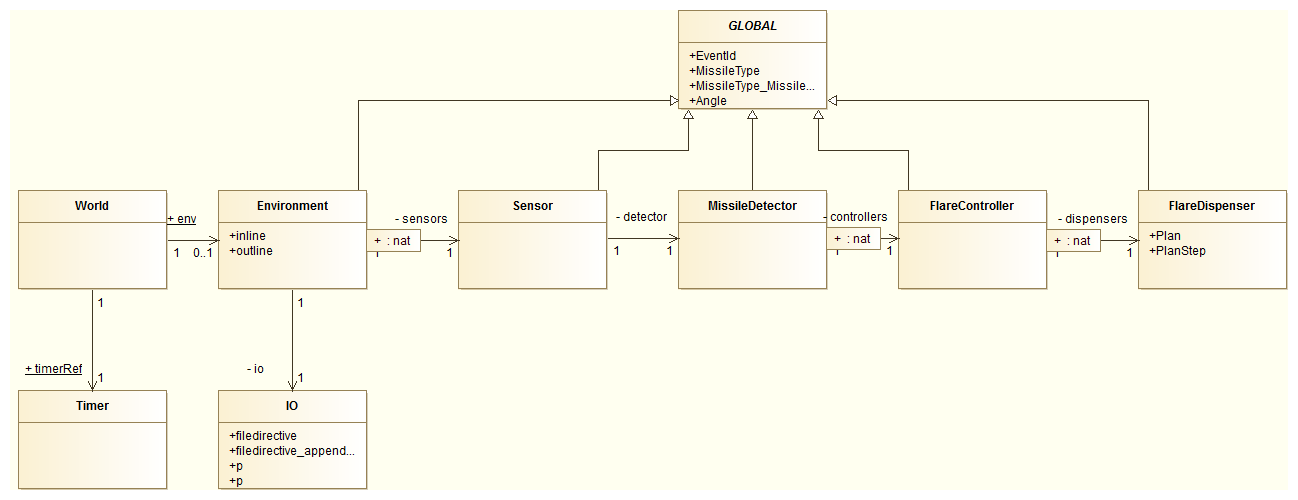
\includegraphics[width=\textwidth]{figures/seqCMclassdiag.png}
\end{center}
\caption{Class Diagram for the Sequential Counter Measures Model\label{fig:classdiagseq}}
\end{figure}

\subsection{The Counter Measures Class}

This is the overall system class called \texttt{CM} corresponding to
the \texttt{SystemName} in Section~\ref{sec:designvice}.
In Section~\ref{sec:VDMSLreq} four different magazines (or flare
dispensers) was used covering 90 degrees each. In reality it is
possible to have different numbers of sensors and actuators. In
principle it is also possible to have overlapping sensors and
actuators redundantly in order to increase fault tolerance for the
overall system. In order to illustrate how this can be done using the
VDM++ framework described in this document a design is presented with
\begin{itemize}
\item four sensors covering 90 degrees of angle each;
\item one missile detector;
\item three flare controllers covering 120 degrees of angle each
controlling four flare dispensers;
\item twelve flare dispensers coping with 30 degrees of each.
\end{itemize}

In this way each flare controller will have four flare dispensers to
control each. As it will be clear below this is a rather complex
system, but it is modelled in a fashion that makes it easy to
reconfigure it to investigate alternative compositions of
sensors, flare controllers and flare dispensers.

In the \texttt{CM} class this is documented as:
\newpage

\begin{lstlisting}
class CM
instance variables

public static 
detector : MissileDetector := new MissileDetector();
public static sensor0 : Sensor := new Sensor(detector,0);
public static sensor1 : Sensor := new Sensor(detector,90);
public static sensor2 : Sensor := new Sensor(detector,180);
public static sensor3 : Sensor := new Sensor(detector,270);
public static 
controller0 : FlareController := new FlareController(0);
public static 
controller1 : FlareController := new FlareController(120);
public static 
controller2 : FlareController := new FlareController(240);
public static 
dispenser0 : FlareDispenser := new FlareDispenser(0);
public static 
dispenser1 : FlareDispenser := new FlareDispenser(30);
public static 
dispenser2 : FlareDispenser := new FlareDispenser(60);
public static 
dispenser3 : FlareDispenser := new FlareDispenser(90);
public static 
dispenser4 : FlareDispenser := new FlareDispenser(0);
public static 
dispenser5 : FlareDispenser := new FlareDispenser(30);
public static 
dispenser6 : FlareDispenser := new FlareDispenser(60);
public static 
dispenser7 : FlareDispenser := new FlareDispenser(90);
public static 
dispenser8 : FlareDispenser := new FlareDispenser(0);
public static 
dispenser9 : FlareDispenser := new FlareDispenser(30);
public static 
dispenser10 : FlareDispenser := new FlareDispenser(60);
public static 
dispenser11 : FlareDispenser := new FlareDispenser(90);

end CM
\end{lstlisting}

\subsection{The World Class}

The \texttt{World} class consists of two static public instance variables and
two operations. The two instance variables refer to the \texttt{env}ironment
and the \texttt{timerRef} to be used by both the environment and system
classes. 

\begin{lstlisting}
class World

instance variables
  
public static 
env : [Environment] := nil;
public static timerRef : Timer := Timer`GetInstance();
\end{lstlisting}

The constructor \texttt{World} is used to set
up the object topology (adding sensors, controller and dispensers to 
the environment, the detector and different controllers respectively).
In principle the \texttt{new Environment} could be made in the 
{\bf\ttfamily{instance variables}} section but that could introduce infinite 
recursion in the initialisation of Overture or \vdmtools.

\begin{lstlisting}
operations

public World: () ==> World
World () ==
 (  -- set-up the sensors
    env := new Environment("scenario.txt");
    env.addSensor(CM`sensor0);
    env.addSensor(CM`sensor1);
    env.addSensor(CM`sensor2);
    env.addSensor(CM`sensor3);

    -- add the first controller with four dispensers
    CM`controller0.addDispenser(CM`dispenser0);
    CM`controller0.addDispenser(CM`dispenser1);
    CM`controller0.addDispenser(CM`dispenser2);
    CM`controller0.addDispenser(CM`dispenser3);
    CM`detector.addController(CM`controller0);

    -- add the second controller with four dispensers
    CM`controller1.addDispenser(CM`dispenser4);
    CM`controller1.addDispenser(CM`dispenser5);
    CM`controller1.addDispenser(CM`dispenser6);
    CM`controller1.addDispenser(CM`dispenser7);
    CM`detector.addController(CM`controller1);
 
    -- add the third controller with four dispensers
    CM`controller2.addDispenser(CM`dispenser8);
    CM`controller2.addDispenser(CM`dispenser9);
    CM`controller2.addDispenser(CM`dispenser10);
    CM`controller2.addDispenser(CM`dispenser11);
    CM`detector.addController(CM`controller2);
   );
\end{lstlisting}

The \texttt{Run} operation is used to execute the model and this is done
by handing over control to the environment. 

\begin{lstlisting}
public Run: () ==> ()
Run () == 
  env.Run()

end World
\end{lstlisting}

\subsection{The Global Class}\label{sec:GlobalSeq}

The \texttt{GLOBAL} class is responsible for providing a common place to
store global definitions of relevance for the rest of the model.

This includes value definitions indicating the number of degrees that can 
be observe (the viewing angle is termed ``aperture''):

\begin{lstlisting}
class GLOBAL

values

public SENSOR_APERTURE = 90;
public FLARE_APERTURE = 120;
public DISPENSER_APERTURE = 30
\end{lstlisting}

It also includes the \texttt{MissileType} and \texttt{FlareType} that
was presented in Section~\ref{subsec:generaltypes} and in addition a 
type for identifying the incoming events \texttt{EventId}.
%\newpage

\begin{lstlisting}
types

public 
MissileType = <MissileA> | <MissileB> | <MissileC> | <None>;

public FlareType =
    <FlareOneA> | <FlareTwoA> | <DoNothingA> | 
    <FlareOneB> | <FlareTwoB> | <DoNothingB> | 
    <FlareOneC> | <FlareTwoC> | <DoNothingC>;

public Angle = nat
inv num == num <= 360;

public EventId = nat;

public Time = nat
\end{lstlisting}

The \texttt{canObserve} operation is used to check whether an
aperture (a sensor, a flare controller or a flare dispenser) 
can observe a missile coming at the \texttt{pangle} angle. Each subclass 
of \texttt{GLOBAL} must supply an operation called \texttt{getAperture}
that will yield a pair of degrees indicating the left hand side that the 
aperture can observe and the number of degrees it can observe.
 
\begin{lstlisting}
operations

public canObserve: Angle * Angle * Angle ==> bool
canObserve (pangle, pleft, psize) ==
  def pright = (pleft + psize) mod 360 in
    if pright < pleft
    -- check between [0,pright> and [pleft,360>
    then return (pangle < pright or pangle >= pleft)
    -- check between [pleft, pright>
    else return (pangle >= pleft and pangle < pright);
       
public getAperture: () ==> Angle * Angle
getAperture () == is subclass responsibility;

end GLOBAL
\end{lstlisting}

\subsection{The Environment Class}

The \texttt{Environment} class is responsible for the interaction with
all the system classes to and from the environment classes. It is
defined as a subclass of \texttt{GLOBAL}. The input and output are sequences of
lines that have types defined for them. The types \texttt{inline} and 
\texttt{outline} are tuples ending with the time at which the event have
appeared (in \texttt{outline} the last two indicate the time which the event 
has been received and dealt with respectively).

\begin{lstlisting}
class Environment is subclass of GLOBAL

types

public inline  = EventId * MissileType * Angle * Time;
public outline = EventId * FlareType * Angle * Time * Time;
\end{lstlisting}

Instance variables exist for performing \texttt{io} in addition to the 
\texttt{inlines} and \texttt{outlines}.

\begin{lstlisting}
-- access to the standard IO library
io : IO := new IO();

inlines : seq of inline := [];

outlines : seq of outline := [];
\end{lstlisting}

The mappings \texttt{ranges} and \texttt{sensors} are used for keeping 
track of the sensors and the angle ranges they are able to observe between.

\begin{lstlisting}
ranges : map nat to (Angle * Angle) := {|->};
sensors : map nat to Sensor := {|->};
inv dom ranges = dom sensors;
\end{lstlisting}

Finally \texttt{evid} and \texttt{busy} are used to keep track of the last 
received event and whether the environment is busy or not respectively.

\begin{lstlisting}
evid : [EventId] := nil;

busy : bool := true;
\end{lstlisting}

The constructor reads a given scenario and the file name is used as parameter.

\begin{lstlisting}
operations

public Environment: seq of char ==> Environment
Environment (fname) ==
 def mk_ (-,input) = io.freadval[seq of inline](fname) in
   inlines := input;
\end{lstlisting}

Sensors must be added to the \texttt{Environment} using the \texttt{addSensor}
operation. Note that in order to ensure the state invariant between 
\texttt{ranges} and \texttt{sensors} an \texttt{atomic} statement is used.

\begin{lstlisting}
public addSensor: Sensor ==> ()
addSensor (psens) ==
  ( dcl id : nat := card dom ranges + 1;
    atomic (
     ranges := ranges munion {id |-> psens.getAperture()};
     sensors := sensors munion {id |-> psens} 
    )
  );
\end{lstlisting}

The \texttt{Run} operation create new signals from the environment and steps 
to the corresponding system reaction until both the system and the environment
are finished with their execution.

\begin{lstlisting}
public Run: () ==> ()
Run () == 
 (while not (isFinished() and CM`detector.isFinished()) do
    (createSignal();
     CM`detector.Step();
     World`timerRef.StepTime();
    );
 showResult()
 );
\end{lstlisting}

The \texttt{createSignal} operation is used for extracting input and
directing it to a sensor that can observe the given input angle \texttt{pa}.
%\newpage

\begin{lstlisting}
private createSignal: () ==> ()
createSignal () ==
  ( if len inlines > 0
    then (dcl curtime : Time := World`timerRef.GetTime(), 
              done : bool := false;
          while not done do
            def mk_ (eventid, pmt, pa, pt) = hd inlines in
              if pt <= curtime
              then (for all id in set dom ranges do
                      def mk_(papplhs,pappsize) = ranges(id) in
                        if canObserve(pa,papplhs,pappsize)
                        then sensors(id).trip(eventid,pmt,pa);
                    inlines := tl inlines;
                    done := len inlines = 0)
              else done := true)
    else busy := false);
\end{lstlisting}

The \texttt{handleEvent} operation is used when the \texttt{CM} classes have
coped with an input event and produced an outgoing event that must be stored.

\begin{lstlisting}
public 
handleEvent: EventId * FlareType * Angle * Time * Time ==> ()
handleEvent (evid,pfltp,angle,pt1,pt2) ==
  (outlines := outlines ^ [mk_ (evid,pfltp, angle,pt1, pt2)] );
\end{lstlisting}

The \texttt{showResult} operation is used to write out the overall result.

\begin{lstlisting}
public showResult: () ==> ()
showResult () ==
  def - = io.writeval[seq of outline](outlines) in skip;
\end{lstlisting}

Finally the \texttt{isFinished} operation is used to check if the 
\texttt{Environment} is finished with its execution.
%\newpage

\begin{lstlisting}
public isFinished : () ==> bool
isFinished () == 
  return inlines = [] and not busy;

end Environment
\end{lstlisting}

\subsection{The Sensor Class}

The \texttt{Sensor} class is used to model the sensor hardware from
the environment. It contains an instance variable \texttt{aperture}
that models the left hand-side of the viewing angle of the sensor.

\begin{lstlisting}
class Sensor is subclass of GLOBAL

instance variables

-- the missile detector this sensor is connected to
private detector : MissileDetector;

-- the left hand-side of the viewing angle of the sensor
private aperture : Angle;
\end{lstlisting}

The constructor initialises the \texttt{aperture} instance variable and the 
\texttt{getAperture} operation uses this information.

\begin{lstlisting}
operations

public Sensor: MissileDetector * Angle ==> Sensor
Sensor (pmd, psa) == (detector := pmd; aperture := psa);

public getAperture: () ==> GLOBAL`Angle * GLOBAL`Angle
getAperture () == return mk_ (aperture, SENSOR_APERTURE);
\end{lstlisting}

The \texttt{trip} operation is called from the \texttt{Environment} to
signal an event. The sensor triggers the missile detector for further 
processing using the \texttt{addThreat} operation. Note that the caller
must ensure that the sensor must be able to observe the given event.
%\newpage

\begin{lstlisting}
public trip: EventId * MissileType * Angle ==> ()
trip (evid, pmt, pa) ==
  -- log and time stamp the observed threat
  CM`detector.addThreat(evid, pmt,pa,World`timerRef.GetTime())
pre canObserve(pa, aperture, SENSOR_APERTURE)

end Sensor
\end{lstlisting}

\subsection{The Missile Detector Class}

The primary task of the \texttt{MissileDetector} class is to
collect all sensor data and dispatch each event
to the appropriate \texttt{FlareController} instance.

In the same way as the \texttt{Environment} class instance variables are 
used for keeping track of the \texttt{ranges} and the \texttt{controllers}.

\begin{lstlisting}
class MissileDetector is subclass of GLOBAL

instance variables

ranges : map nat to (Angle * Angle) := {|->};
controllers : map nat to FlareController := {|->};
inv dom ranges = dom controllers;
\end{lstlisting}

The \texttt{threats} instance variable collects the observations from 
all attached sensors and \texttt{busy} keeps track of the status of
the \texttt{MissileDetector}.

\begin{lstlisting}
threats : seq of (EventId * MissileType * Angle * Time) := [];

busy : bool := false
\end{lstlisting}

The \texttt{addController} operation is only used to instantiate the model
%\newpage

\begin{lstlisting}
operations

public addController: FlareController ==> ()
addController (pctrl) ==
  (dcl nid : nat := card dom ranges + 1;
   atomic
    (ranges := ranges munion {nid |-> pctrl.getAperture()};
     controllers := controllers munion {nid |-> pctrl}
    );
  );
\end{lstlisting}

The operation \texttt{Step} is used to ``step'' the algorithm: it
takes threats and finds the right controller to relay the threat to
and calls \texttt{addThreat} on the appropriate controller instance. It 
also need to ensure that all controllers will take a \texttt{Step} in their
own processing.

\begin{lstlisting}
public Step: () ==> ()
Step() ==
  (if threats <> []
   then def mk_ (evid,pmt, pa, pt) = getThreat() in
          for all id in set dom ranges do
            def mk_(papplhs, pappsize) = ranges(id) in
              if canObserve(pa, papplhs, pappsize)
              then controllers(id).addThreat(evid,pmt,pa,pt);
    busy := len threats > 0;
    for all id in set dom controllers do
      controllers(id).Step()
  );
\end{lstlisting}

The \texttt{addThreat} operation is used to modify the event
list. In the current model events are stored first come first served,
but one could imagine using a different ordering instead.
%\newpage

\begin{lstlisting}
public addThreat: EventId * MissileType * Angle * Time ==> ()
addThreat (evid,pmt,pa,pt) == 
  (threats := threats ^ [mk_ (evid,pmt,pa,pt)];
   busy := true );
\end{lstlisting}

The \texttt{getThreat} operation is a local helper operation to modify the event list.
Finally the \texttt{isFinished} operation is defined such that it is finished when
all the controllers are finished.

\begin{lstlisting}
private getThreat: () ==> EventId * MissileType * Angle * Time
getThreat () ==
  (dcl res : EventId * MissileType * Angle * Time 
           := hd threats;
   threats := tl threats;
   return res );

public isFinished: () ==> bool
isFinished () ==
  return forall id in set dom controllers &
            controllers(id).isFinished()

end MissileDetector
\end{lstlisting}

\subsection{The Flare Controller Class}

The job of the \texttt{FlareController} class is to determine which flare
dispenser to relay the incoming threat to the right flare dispenser.

Like the \texttt{Sensor} class it has \texttt{aperture} as an instance 
variable to keep track of the left-hand-side of its working angle. 
In addition, it maintains a link to all its flare dispensers using the 
same scheme as for \texttt{MissileDetector} and the \texttt{Environment}
classes.

\begin{lstlisting}
class FlareController is subclass of GLOBAL

instance variables

private aperture : Angle;

ranges : map nat to (Angle * Angle) := {|->};
dispensers : map nat to FlareDispenser := {|->};
inv dom ranges = dom dispensers;
\end{lstlisting}

Just like the \texttt{MissileDetector} class it includes the \texttt{threats} and
\texttt{busy} instance variables.

\begin{lstlisting}
-- the relevant events to be treated by this controller
threats : seq of (EventId * MissileType * Angle * Time) := [];

-- the status of the controller
busy : bool := false
\end{lstlisting}

The constructor is setting the \texttt{aperture} instance variable in the 
same fashion as the \texttt{Sensor} class. The \texttt{addDispenser}
operation is similar to the \texttt{addController} and \texttt{addSensor}
from the \texttt{MissileDetector} and the \texttt{Environment} classes 
respectively.

\begin{lstlisting}
operations

public FlareController: Angle ==> FlareController
FlareController (papp) == aperture := papp;

public addDispenser: FlareDispenser ==> ()
addDispenser (pfldisp) ==
  let angle = aperture + pfldisp.GetAngle() in
    (dcl id : nat := card dom ranges + 1;
     atomic
     (ranges := ranges munion 
                {id |-> mk_(angle, DISPENSER_APERTURE)};
      dispensers := dispensers munion {id |-> pfldisp});
     );
\end{lstlisting}

The operation \texttt{Step} is used to ``step'' the algorithm in the
same way as the \texttt{Step} operation from the \texttt{MissileDetector}
class: it
takes threats and finds the right dispenser to relay the threat to
and calls \texttt{addThreat} on the appropriate dispenser instance. It 
also need to ensure that all dispensers will take a \texttt{Step} in their
own processing.

\begin{lstlisting}
public Step: () ==> ()
Step() ==
  (if threats <> []
   then def mk_ (evid,pmt, pa, pt) = getThreat() in
          for all id in set dom ranges do
            def mk_(papplhs, pappsize) = ranges(id) in
              if canObserve(pa, papplhs, pappsize)
              then dispensers(id).addThreat(evid,pmt,pt);
   busy := len threats > 0;
   for all id in set dom dispensers do
     dispensers(id).Step());
\end{lstlisting}

The \texttt{getAperture} operation gets the left hand-side start point 
and opening angle and yield a pair of angles in the same way as
\texttt{getAperture} from the \texttt{Sensor} class.

\begin{lstlisting}
public getAperture: () ==> GLOBAL`Angle * GLOBAL`Angle
getAperture () == return mk_(aperture, FLARE_APERTURE);
\end{lstlisting}

Just like the \texttt{MissileDetector} class the \texttt{addThreat},
\texttt{getThreat} and
\texttt{isFinshed} operations are present here.

\begin{lstlisting}
public addThreat: EventId * MissileType * Angle * Time ==> ()
addThreat (evid,pmt,pa,pt) ==
  (threats := threats ^ [mk_ (evid,pmt,pa,pt)];
   busy := true );

private getThreat: () ==> EventId * MissileType * Angle * Time
getThreat () ==
  (dcl res : EventId * MissileType * Angle * Time 
           := hd threats;
   threats := tl threats;
   return res );

public isFinished: () ==> bool
isFinished () ==
  return forall id in set dom dispensers &
            dispensers(id).isFinished();

end FlareController
\end{lstlisting}

\subsection{The Flare Dispenser Class}

The \texttt{FlareDispenser} class is responsible for firing the actual
flares according to the plan for the given missile id. The \texttt{responseDB}
value contains a mapping from \texttt{MissileType} to such a \texttt{Plan}.
 
\begin{lstlisting}
class FlareDispenser is subclass of GLOBAL

values

responseDB : map MissileType to Plan =
  {<MissileA> |-> [mk_(<FlareOneA>,900),
                   mk_(<FlareTwoA>,500),
                   mk_(<DoNothingA>,100),
                   mk_(<FlareOneA>,500)],
   <MissileB> |-> [mk_(<FlareTwoB>,500),
                   mk_(<FlareTwoB>,700)],
   <MissileC> |-> [mk_(<FlareOneC>,400),
                   mk_(<DoNothingC>,100),
                   mk_(<FlareTwoC>,400),
                   mk_(<FlareOneC>,500)] };
\end{lstlisting}

In the same way the \texttt{missilePriority} provides information about 
the priority for the different types of missiles.

\begin{lstlisting}
missilePriority : map MissileType to Time =
  { <None>     |-> 0,
    <MissileA> |-> 1,
    <MissileB> |-> 2,
    <MissileC> |-> 3 }
\end{lstlisting}

\texttt{Plan}'s are structured as a sequence of \texttt{PlanStep}'s.

\begin{lstlisting}
types

public Plan = seq of PlanStep;

public PlanStep = FlareType * Time;
\end{lstlisting}

\texttt{FlareDispenser} contains a number of instance variables for 
keeping track of the current status of the flare dispenser.

\begin{lstlisting}
instance variables

public curplan : Plan := [];
curprio        : nat  := 0;
busy           : bool := false;
aperture       : Angle;
eventid        : [EventId];
\end{lstlisting}

The constructor sets the \texttt{aperture} instance variable in the 
same way as for the constructor of the \texttt{Sensor} and
\texttt{FlareController} classes. The \texttt{GetAngle} provides the 
\texttt{aperture} in the usual fashion.

\begin{lstlisting}
operations

public FlareDispenser: nat ==> FlareDispenser
FlareDispenser(ang) ==
  aperture := ang;

public GetAngle: () ==> nat
GetAngle() ==
  return aperture;
\end{lstlisting}

The \texttt{Step} operation is similar to what is found in the 
\texttt{MissileDetector} and \texttt{Flare\-Controller} classes except that 
here actual flares are released rather than relaying the information to
yet another class.

\begin{lstlisting}
public Step: () ==> ()
Step() ==
  if len curplan > 0
  then (dcl curtime : Time := World`timerRef.GetTime(),
            first : PlanStep := hd curplan,
            next : Plan := tl curplan;
        let mk_(fltp, fltime) = first in
          (if fltime <= curtime
           then (releaseFlare(eventid,fltp,fltime,curtime);
                 curplan := next;
                 if len next = 0
                 then (curprio := 0; 
                       busy := false ) )
           )
    );
\end{lstlisting}

The \texttt{addThreat} operation is used from the
\texttt{Flare}-\texttt{Controller}'s  
to insert the event of a new missile detected. Here the priority of the
missile is essential to determine whether any existing treatment of another
missile shall be interrupted.

\begin{lstlisting}
public addThreat: EventId * MissileType * Time ==> ()
addThreat (evid, pmt, ptime) ==
  if missilePriority(pmt) > curprio
  then (dcl newplan : Plan :=  [],
            newtime : Time := ptime;
        -- construct an absolute time plan
        for mk_(fltp, fltime) in responseDB(pmt) do
          (newplan := newplan ^ [mk_ (fltp, newtime)];
           newtime := newtime + fltime );
        -- immediately release the first action
        def mk_(fltp, fltime) = hd newplan;
            t = World`timerRef.GetTime() in
          releaseFlare(evid,fltp,fltime,t);
        -- store the rest of the plan
        curplan := tl newplan;
        eventid := evid;
        curprio := missilePriority(pmt);
        busy := true )
pre pmt in set dom missilePriority and
    pmt in set dom responseDB;
\end{lstlisting}

The \texttt{releaseFlare} operation is simply communicating to the 
environment using the operation called \texttt{handleEvent} from the \texttt{Environment} 
class.

\begin{lstlisting}
private releaseFlare: EventId * FlareType * Time * Time ==> ()
releaseFlare (evid,pfltp, pt1, pt2) == 
  World`env.handleEvent(evid,pfltp,aperture,pt1,pt2);
\end{lstlisting}

Finally the \texttt{isFinished} operation is defined in terms of checking
whether the operation \texttt{FlareDispenser} is busy.

\begin{lstlisting}
public isFinished: () ==> bool
isFinished () == 
  return not busy

end FlareDispenser
\end{lstlisting}

\subsection{The Timer Class}\label{sec:timerclass}

The \texttt{Timer} class is used to control evolution of time
throughout the sequential model. To get an unambiguous notion of time, it is important that only a single instance of this class exists. For this reason, the class is following the singleton pattern. The constructor of the class is {\bf\ttfamily{private}}, so all classes in the system that needs to access time must use the operation \texttt{GetInstance} to get the singleton instance.

\begin{lstlisting}
class Timer

instance variables

private static timerInstance : Timer := new Timer(); 

operations

private Timer: () ==> Timer
Timer() ==
  skip;
  
public static GetInstance: () ==> Timer
GetInstance() ==
  return timerInstance;
\end{lstlisting}

The \texttt{Timer} has one instance variable called
\texttt{currentTime} representing the current time in the system. 

\begin{lstlisting}
class Timer

instance variables

currentTime : nat := 0;
\end{lstlisting}

Time is incremented in the system in units of the constant value
\texttt{stepLength}.

\begin{lstlisting}
values

stepLength : nat = 100;
\end{lstlisting}

The operation \texttt{StepTime} is used to progress time in the system.

\begin{lstlisting}
public StepTime : () ==> ()
StepTime() ==
  currentTime := currentTime + stepLength;
\end{lstlisting}

The operation \texttt{GetTime} is used to read the current time.

\begin{lstlisting}
public GetTime : () ==> nat
GetTime() ==
  return currentTime;

end Timer
\end{lstlisting}

\subsection{The IO Class}

The class \texttt{IO} is the VDM++ standard input/output library. It
needs no further explanation.

\begin{lstlisting}
class IO

-- 	Overture STANDARD LIBRARY: INPUT/OUTPUT
--      --------------------------------------------
-- 
-- Standard library for the Overture Interpreter. When the interpreter
-- evaluates the preliminary functions/operations in this file,
-- corresponding internal functions is called instead of issuing a run
-- time error. Signatures should not be changed, as well as name of
-- module (VDM-SL) or class (VDM++). Pre/post conditions is 
-- fully user customisable. 
-- Dont care's may NOT be used in the parameter lists.
--
-- The in/out functions  will return false if an error occurs. In this
-- case an internal error string will be set (see 'ferror').

types
 
public
filedirective = <start>|<append> 

functions

-- Write VDM value in ASCII format to std out:
public
writeval[@p]: @p -> bool
writeval(val)==
  is not yet specified;

-- Write VDM value in ASCII format to file.
-- fdir = <start> will overwrite existing file,
-- fdir = <append> will append output to the file (created if
-- not existing).
public
fwriteval[@p]:seq1 of char * @p * filedirective -> bool
fwriteval(filename,val,fdir) ==
  is not yet specified;

-- Read VDM value in ASCII format from file
public
freadval[@p]:seq1 of char -> bool * [@p]
freadval(f) ==
  is not yet specified
  post let mk_(b,t) = RESULT in not b => t = nil;

operations

-- Write text to std out. Surrounding double quotes will be stripped,
-- backslashed characters should be interpreted.
public
echo: seq of char ==> bool
echo(text) ==
  fecho ("",text,nil);

-- Write text to file like 'echo'
public
fecho: seq of char * seq of char * [filedirective] ==> bool
fecho (filename,text,fdir) ==
  is not yet specified
  pre filename = "" <=> fdir = nil;

-- The in/out functions  will return false if an error occur. In this
-- case an internal error string will be set. 'ferror' returns this
-- string and set it to "".
public
ferror:()  ==> seq of char
ferror () ==
  is not yet specified;
  
-- New simplified format printing operations
-- The questionmark in the signature simply means any type
public static print: ? ==> ()
print(arg) ==
  is not yet specified;

-- New simplified format printing operations
-- The questionmark in the signature simply means any type
public static printf: seq of char * seq of ? ==> ()
printf(format, args) ==
  is not yet specified;

end IO
\end{lstlisting}

\subsection{Validation of the Model}

As for the VDM-SL model there is a need to validate the correct behaviour
of the sequential VDM++ model presented above. In this case the input
and output is done using the standard \texttt{IO} class. Thus one needs
to make updates to the \texttt{scenario.txt} file to test the model with
new possible input. Again one would start this by providing simple test
cases and then gradually make them more and more complex. In this case
the validation of the correct behaviour is complicated by the 
\texttt{FlareDispenser}'s coping with different angles (because their 
angles are relative to the \texttt{FlareController} they are assigned to)
will report their own angle only. We leave it as an exercise for the
reader to update the model to yield the real angle (combining the angle
for the \texttt{FlareController} and the \texttt{FlareDispenser}).

There is a rather complex \texttt{scenario.txt} available in the electronic
version of this model on the web that is sufficient to ensure that all parts of the
model have been exercised at least once just by interpreting
\texttt{new World().Run()}. Again is this documented using the
test coverage feature from Overture. In this sequential model in VDM++
there is still a considerable amount of
abstracting away from different timing delays. However, it still makes
sense to inspect the specific timing requirements for the system 
(listed as item 3 and 4 on page~\pageref{timereq34}). Both of these
timing requirements are also validated with the given scenarios.

\subsection{Summary}

In Section~\ref{sec:seqVDM} a more design-oriented model of the
counter measures system has been presented. This model breaks the
system into its static components (classes) but it does not yet deal
with the dynamic architecture (threads). The main virtue of this model
is the emphasis on functionally correct behaviour using the envisaged
static components.  The precision of the model here enables validation
using traditional testing techniques.

This model was tested with test cases conceptually identical to those
used for the VDM-SL model in Section~\ref{sec:VDMSLreq}.  In this way
the old test cases were reused during host acceptance testing, and the
VDM-SL model was used as an oracle to compare the functional behaviour
of this sequential VDM++ model. Whenever one is reusing such test
cases it may be necessary to include more test cases to achieve the
desired test coverage for the new model.

What can be learnt from this sequential design model is
that we now have a common understanding of the general structural
break down of the counter measures system into its static
components. In addition we have validated that the new model
functionally corresponds to the behaviour described at the more
abstract level in Section~\ref{sec:VDMSLreq}. 

\section{Concurrent VDM++ Design Model}\label{sec:concurmod}

In this section the focus will be on the differences that has been
made to the sequential counter measures model to achieve a concurrent
design model. A full listing of all the classes is present in 
Appendix~\ref{app:concurCM} and an overview of the new class diagram
is given in Figure~\ref{fig:classdiagconcur}.

From the sequential model four of the classes will get active threads
because they have independent computations that can be carried
out. These are the \texttt{Environment}, the
\texttt{Missile\-Detector}, the \texttt{FlareController} and the
\texttt{FlareDispenser} classes. Note that this includes the class 
that had the overall control in the sequential model (\texttt{Environment}) 
and all the classes that had a \texttt{Step} operation.

In addition to these changes the way timing is treated is changed so
the \texttt{Timer} class is replaced with a more elaborate treatment
of time. This is done using the
\texttt{TimeStamp} class and the \texttt{BaseThread} class, 
which may be reused directly for other 
concurrent VDM++ models following the same principles.

Communication occurs between the sensor and the missile detector
(unidirectional) and between the missile detector and the flare
controller (bidirectional). To ensure correct sequencing of the
communication, synchronization is used.

We now present the concurrent model on a class by class basis. The
classes \texttt{GLOBAL}, \texttt{Sensor} and \texttt{IO} 
are unchanged from the
previous model, so are not given again here.

\begin{figure}
\begin{center}
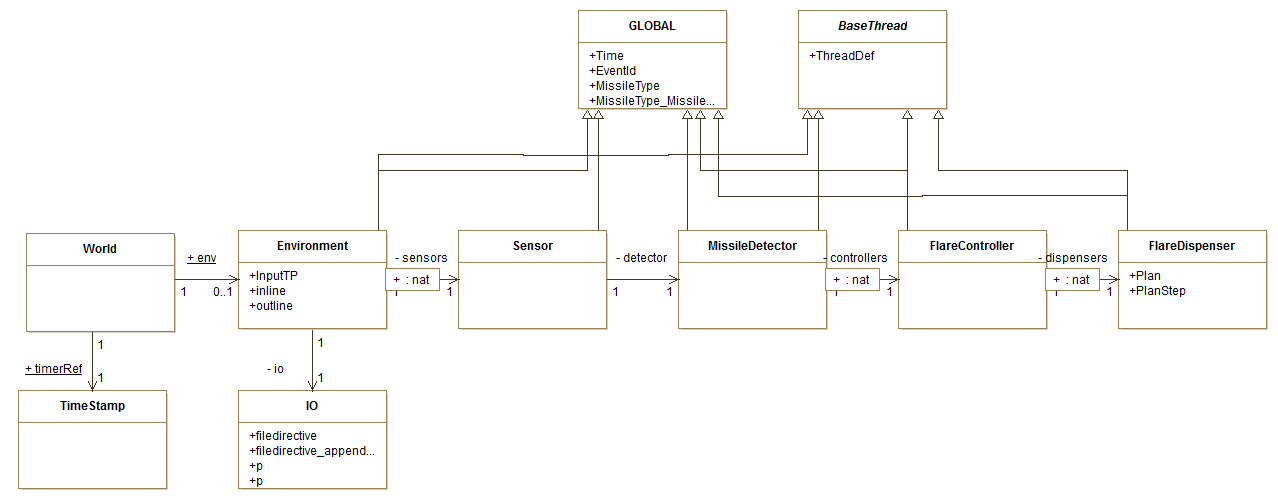
\includegraphics[width=\textwidth]{figures/concurCMclassdiag.png}
\end{center}
\caption{Class Diagram for the Concurrent Counter Measures Model\label{fig:classdiagconcur}}
\end{figure}

\subsection{Introducing the BaseThread and TimeStamp Classes}

In order to ensure that the different active instances get a chance of
stepping in sync with each other both a \texttt{BaseThread} and a
\texttt{TimeStamp} class needs to be introduced. The \texttt{BaseThread}
class is used as a superclass for all active classes that need a chance to 
take a step. It is able to handle both periodic as well as aperiodic threads.
It is defined as:

\begin{lstlisting}
class BaseThread
	
types

public static ThreadDef ::
  p : nat1
  isP : bool;

instance variables

protected period : nat1 := 1;
protected isPeriodic : bool := true;

protected registeredSelf : BaseThread;
protected timeStamp : TimeStamp := TimeStamp`GetInstance();

operations

protected BaseThread : BaseThread ==> BaseThread
BaseThread(t) ==
 (registeredSelf:= t;
  timeStamp.RegisterThread(registeredSelf);
  if(not timeStamp.IsInitialising())
  then start(registeredSelf);  
 );
\end{lstlisting}
\noindent Note how threads get started in the constructor if we are not
initialising the overall collection of classes. For this to happen correctly, all classes inheriting from \texttt{BaseThread} must call the super-constructor explicitly passing a reference to {\bf\ttfamily{self}}. An example of this can be seen in the \texttt{Environment} class, which also shows how to change the default values of the instance variables \texttt{p} specifying the length of a period and \texttt{isP} that specifies if the thread is periodic or not.

\begin{lstlisting}
class Environment is subclass of BaseThread

operations

public Environment: seq of char * [ThreadDef] ==> Environment
Environment (fname, tDef) ==
 (if tDef <> nil
  then (period := tDef.p;
        isPeriodic := tDef.isP;
       );
  BaseThread(self);
  );
\end{lstlisting}

All subclasses of the \texttt{BaseThread} class need to have a \texttt{Step}
operation implementing the abstract operation defined in \texttt{BaseThread}.

\begin{lstlisting}
Step : () ==> ()
Step() ==
  is subclass responsibility
\end{lstlisting}

The active thread depends upon whether we have a periodic thread or not:

\begin{lstlisting}
thread
 (if isPeriodic
  then (while true
        do 
         (Step();
          timeStamp.WaitRelative(period);
         )
       )
  else (Step();
        World`timerRef.WaitRelative(0);
        timeStamp.UnRegisterThread(registeredSelf);
       )
 );

end BaseThread
\end{lstlisting}

The \texttt{TimeStamp} singleton class maintains a map from thread ids to 
time (\texttt{wakeUpMap}), representing when a particular thread 
should be woken. The other instance variable in the class
represents the current time. Note that this concept is orthogonal to
the notion of simulated time described earlier in this document.

\begin{figure}
\begin{center}
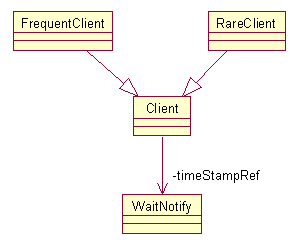
\includegraphics[width=0.5\textwidth]{figures/timestamp.png}
\end{center}
\caption{Class Diagram for Time Stamp Pattern\label{fig:classtimestamp}}
\end{figure}

%\begin{figure}
%\begin{center}
%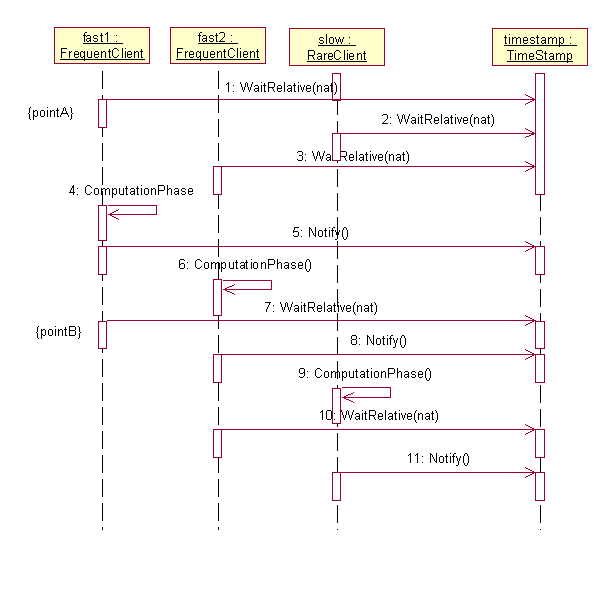
\includegraphics[width=\textwidth]{figures/timestampseqdiag.png}
%\end{center}
%\caption{Sequence Diagram for Time Stamp Pattern\label{fig:seqdiagtimestamp}}
%\end{figure}

\begin{lstlisting}
class TimeStamp

values

public stepLength : nat = 1;

instance variables

currentTime  : nat   := 0;
wakeUpMap    : map nat to [nat] := {|->};
barrierCount : nat := 0;
registeredThreads : set of BaseThread := {};
isInitialising : bool := true;
-- singleton instance of class
private static timeStamp : TimeStamp := new TimeStamp();
\end{lstlisting}

To get the singleton instance of the \texttt{TimeStamp} class the operation \texttt{GetInstance} is called.

\begin{lstlisting}
operations

-- private constructor (singleton pattern)
private TimeStamp : () ==> TimeStamp
TimeStamp() ==
  skip;

-- public operation to get the singleton instance
public static GetInstance: () ==> TimeStamp
GetInstance() ==
  return timeStamp;
\end{lstlisting}

Whenever a thread is started it gets registered with a reference to it. This happens automatically in the constructor of the \texttt{BaseThread}.

\begin{lstlisting}
public RegisterThread : BaseThread ==> ()
RegisterThread(t) ==
 (barrierCount := barrierCount + 1;
  registeredThreads := registeredThreads union {t};  
 );
 
public UnRegisterThread : BaseThread ==> ()
UnRegisterThread(t) ==
 (barrierCount := barrierCount - 1;
  registeredThreads := registeredThreads \ {t};
 );
\end{lstlisting}

When all threads have registered themselves and initialisation is finished
all these threads can be started by explicitly calling the operation \texttt{DoneInitialising}.

\begin{lstlisting}
public IsInitialising: () ==> bool
IsInitialising() ==
  return isInitialising;
 
public DoneInitialising: () ==> ()
DoneInitialising() ==
 (if isInitialising
  then (isInitialising := false;
        for all t in set registeredThreads 
        do
          start(t);
       );
 );
\end{lstlisting}

To model periodic behaviour, a client can be put to sleep using \texttt{WaitRelative}.

\begin{lstlisting}
public WaitRelative : nat ==> ()
WaitRelative(val) ==
  WaitAbsolute(currentTime + val);
\end{lstlisting}

Absolute waits are performed using \texttt{WaitAbsolute}. Note that if time
given is less than the current time, then the client will never be
woken.

\begin{lstlisting}
public WaitAbsolute : nat ==> ()
WaitAbsolute(val) ==
 (AddToWakeUpMap(threadid, val);
  -- Last to enter the barrier notifies the rest.
  BarrierReached();
  -- Wait till time is up
  Awake();
);
\end{lstlisting}

\texttt{AddToWakeUpMap} is used to add new waits to the \texttt{wakeUpMap}.

\begin{lstlisting}
AddToWakeUpMap : nat * nat ==> ()
AddToWakeUpMap(tId, val) ==
  wakeUpMap := wakeUpMap ++ { tId |-> val };
\end{lstlisting}

The operation \texttt{BarrierReached} evaluates the \texttt{wakeUpMap} when 
all period threads have entered the mapping. Time is incremented and all threads
that needs to be awoken is removed from the \texttt{wakeUpMap}.

\begin{lstlisting}
BarrierReached : () ==> ()
BarrierReached() == 
  while  (card dom wakeUpMap = barrierCount) do
   (currentTime := currentTime + stepLength;
    let threadSet : set of nat = {th | th in set dom wakeUpMap 
                                     & wakeUpMap(th) <> nil and 
                                       wakeUpMap(th) <= currentTime }
    in
      for all t in set threadSet 
      do
         wakeUpMap := {t} <-: wakeUpMap;
   )
post forall x in set rng wakeUpMap & x = nil or x >= currentTime;
\end{lstlisting}

All threads block on the operation \texttt{Awake} until they are removed from
the \texttt{wakeUpMap} as described above.

\begin{lstlisting}
operations

Awake: () ==> ()
Awake() == skip;

sync
  per Awake => threadid not in set dom wakeUpMap;
\end{lstlisting}

The current time of the class may be obtained via the \texttt{GetTime}
operation.

\begin{lstlisting}
public GetTime : () ==> nat
GetTime() ==
  return currentTime;
\end{lstlisting}

Since \texttt{barrierCount}, \texttt{registeredThreads} and 
\texttt{wakeUpMap} is manipulated by a number of different
operations, we need to set access to them to be mutually exclusive.

\begin{lstlisting}
sync
  mutex(IsInitialising);
  mutex(DoneInitialising);
  mutex(AddToWakeUpMap);
  mutex(NotifyThread);
  mutex(BarrierReached);
  mutex(AddToWakeUpMap, NotifyThread);
  mutex(AddToWakeUpMap, BarrierReached);
  mutex(NotifyThread, BarrierReached);
  mutex(AddToWakeUpMap, NotifyThread, BarrierReached);

end TimeStamp
\end{lstlisting}

\subsection{Updating the CM Class}

All constructors from classes that need to be active must be updated
with extra parameters indicating if they are periodic and if so what
the required period is. This update of the constructors needs to be
used inside the \texttt{CM} class. In this case we wish them all to 
be periodic with a period of one time unit. Thus CM becomes:

\begin{lstlisting}
class CM
 
instance variables

-- maintain a link to the detector
public static detector : MissileDetector := new MissileDetector(1, true);

-- sensors are unchanged
public static controller0 : FlareController := new FlareController(0, 1, true);
public static controller1 : FlareController := 
                             new FlareController(120, 1, true);
public static controller2 : FlareController := 
                             new FlareController(240, 1, true);

public static dispenser0 : FlareDispenser := new FlareDispenser(0, 1, true);
public static dispenser1 : FlareDispenser := new FlareDispenser(30, 1, true);
public static dispenser2 : FlareDispenser := new FlareDispenser(60, 1, true);
public static dispenser3 : FlareDispenser := new FlareDispenser(90, 1, true);

public static dispenser4 : FlareDispenser := new FlareDispenser(0, 1, true);
public static dispenser5 : FlareDispenser := new FlareDispenser(30, 1, true);
public static dispenser6 : FlareDispenser := new FlareDispenser(60, 1, true);
public static dispenser7 : FlareDispenser := new FlareDispenser(90, 1, true);

public static dispenser8 : FlareDispenser := new FlareDispenser(0, 1, true);
public static dispenser9 : FlareDispenser := new FlareDispenser(30, 1, true);
public static dispenser10 : FlareDispenser := new FlareDispenser(60, 1, true);
public static dispenser11 : FlareDispenser := new FlareDispenser(90, 1, true);

end CM
\end{lstlisting}

\subsection{Updating the World Class}

The \texttt{timerRef} instance variable is changed from a reference to 
the \texttt{Timer} class to a reference to the \texttt{TimeStamp} singleton class.
This is done in order to synchronize properly between the different 
independent threads.

%% The constructor of the \texttt{World} class is unchanged from the 
%% previous model except that at the end there is a start statement
%% for the statically declared \texttt{detector} from the \texttt{CM} class.

%% \begin{lstlisting}
%% start(CM`detector)
%% \end{lstlisting}

However the \texttt{Run} operation is drastically changed to indicate that now initialisation is complete. Thus, it now becomes:

\begin{lstlisting}
-- the run function blocks the user-interface thread
-- until all missiles in the file have been processed
public Run: () ==> ()
Run () == 
  (timerRef.DoneInitialising();
   -- wait for the environment to handle all input
   env.isFinished();
   -- wait for the missile detector to finish
   CM`detector.isFinished();
   -- print the result
   env.showResult())
\end{lstlisting}

Note how this new definition relies upon the different operations
having permission predicates defined such that they are blocked until
they are indeed ready to perform the desired action.

\subsection{Updating the Environment Class}

The \texttt{Environment} class needs to be declared active so it must 
now inherit from the \texttt{BaseThread} class:

\begin{lstlisting}
class Environment is subclass of GLOBAL, BaseThread
\end{lstlisting}

In addition the \texttt{Run} operation is
replaced with a \texttt{Step} operation. This looks like:

\begin{lstlisting}
public Step : () ==> ()
Step() ==
 (if World`timerRef.GetTime() < simtime
  then createSignal()
  else busy := false;
 );
\end{lstlisting}

In essence \texttt{Step} here is similar but a bit simpler than the
\texttt{Run} operation. Note that a
new instance variable called \texttt{simtime} is introduced. It is
defined as:

\begin{lstlisting}
simtime : Time;
\end{lstlisting}
and it is initialised in the \texttt{Environment} constructor. This
is used to simulate how long time we at most wish to simulate the
entire system. Actually in a case like the CM example where the system
only needs to respond to input events present in the
\texttt{Environment} it is not strictly needed, but since we would
also like to be able to describe reactive systems where the system to
be designed is able to react to the absence of events from the
\texttt{Environment} this kind of principle needs to be introduced
because in that case it would be needed. The constructor is also extended 
with information about its period so it now looks like:

\begin{lstlisting}
public Environment: seq of char * [ThreadDef] ==> Environment
Environment (fname, tDef) ==
 (def mk_ (-,mk_(timeval,input)) = io.freadval[InputTP](fname) in
    (inlines := input;
     simtime := timeval);
     
  if tDef <> nil
  then (period := tDef.p;
        isPeriodic := tDef.isP;
       );
  BaseThread(self);
  );
\end{lstlisting}
\noindent where \texttt{period} and \texttt{isPeriodic} are new instance
variables declared in the \texttt{BaseThread} superclass.

The \texttt{isFinished} operation is also simplified by moving its
predicate into a permission predicate. Finally a synchronisation
constraint is made for the operations called
\texttt{handleEvent} and \texttt{createSignal}
ensuring that they cannot be invoked if they
are already running (the {\bf\ttfamily{mutex}} predicates in the
{\bf\ttfamily{sync}} 
section below).

\begin{lstlisting}
public isFinished : () ==> ()
isFinished () == skip;

sync

mutex (handleEvent);
mutex (createSignal);
per isFinished => not busy;
\end{lstlisting}

\subsection{Updating the Missile Detector Class}

Just like for the \texttt{Environment} class the \texttt{MissileDetector} 
class needs to inherit from the \texttt{BaseThread} class:

\begin{lstlisting}
class MissileDetector is subclass of GLOBAL, BaseThread
\end{lstlisting}
\noindent In the same way the constructor is extended with the periodic
information.
%The \texttt{addController} operation definition looks like:
%
%\begin{lstlisting}
%public addController: FlareController ==> ()
%addController (pctrl) ==
%  (dcl nid : nat := card dom ranges + 1;
%   atomic
%    (ranges := ranges munion {nid |-> pctrl.getAperture()};
%     controllers := controllers munion {nid |-> pctrl}
%    );
%   );
%\end{lstlisting}

The \texttt{Step} operation is split into a test and an auxiliary operation
called \texttt{processSensor}:

\begin{lstlisting} 
public Step: () ==> ()
Step() ==
  if len threats > 0
  then processSensor();

processSensor: () ==> ()
processSensor() ==
( def mk_ (evid,pmt, pa, pt) = getThreat() in
     for all id in set dom ranges do
       def mk_(papplhs, pappsize) = ranges(id) in
         if canObserve(pa, papplhs, pappsize)
         then controllers(id).addThreat(evid,pmt,pa,pt);
   busy := len threats > 0);
\end{lstlisting}

The operation \texttt{isFinished} is different from the sequential
model, since it uses a permission predicate to block until the thread
has finished. This means that the {\bf\ttfamily{for all}} quantification is
changed to a loop over all the \texttt{controllers}.

\begin{lstlisting}
public isFinished: () ==> ()
isFinished () ==
  for all id in set dom controllers do
    controllers(id).isFinished()
\end{lstlisting}

From a synchronisation point of view the \texttt{Step} and \texttt{processSensor} operations need to be protected. In the same way the \texttt{addThreat} and 
\texttt{getThreat} operations modify the same instance variables and
therefore they need to be declared mutual exclusive using a
{\bf\ttfamily{mutex}} 
predicate. In addition a permission predicate is introduced for the
\texttt{getThreat} and the \texttt{isFinished} operations. 
\texttt{getThreat} is used as a ``blocking read'' from the main
thread of control of the \texttt{MissileDetector}.

\begin{lstlisting}
sync

mutex (Step);
mutex (processSensor);
mutex (addThreat,getThreat);

per getThreat => len threats > 0;
per isFinished => not busy
\end{lstlisting}

\subsection{Updating the Flare Controller Class}

%The \texttt{addDispenser} operation definition now looks like:
%
%\begin{lstlisting}
%public addDispenser: FlareDispenser ==> ()
%addDispenser (pfldisp) ==
%  let angle = aperture + pfldisp.GetAngle() in
%    (dcl id : nat := card dom ranges + 1;
%     atomic
%      (ranges := ranges munion 
%                 {id |-> mk_(angle, DISPENSER_APERTURE)};
%       dispensers := dispensers munion {id |-> pfldisp});
%     );
%\end{lstlisting}

Just like for the \texttt{MissileDetector} class also needs to inherit
from the \texttt{BaseThread} class. In addition the \texttt{Step}
operation is adjusted in a fashion similar to what we saw for the
\texttt{Missile\-Detector} class:

\begin{lstlisting}
operations

public Step: () ==> ()
Step() ==
  if len threats > 0
  then processThreat();

processThreat: () ==> ()
processThreat() ==
  (def mk_ (evid,pmt, pa, pt) = getThreat() in
      for all id in set dom ranges do
        def mk_(papplhs, pappsize) = ranges(id) in
          if canObserve(pa, papplhs, pappsize)
          then dispensers(id).addThreat(evid,pmt,pt);
    busy := len threats > 0 );
\end{lstlisting}

The operation \texttt{isFinished} is different from the sequential
model, since it uses a permission predicate to block until the thread
has finished. This means that the {\bf\ttfamily{forall}} quantification is
changed to a loop over all the \texttt{dispensers}.

\begin{lstlisting}
public isFinished: () ==> ()
isFinished () ==
  for all id in set dom dispensers do
    dispensers(id).isFinished();
\end{lstlisting}

From a synchronisation point of view \texttt{addThreat} and 
\texttt{getThreat} modify the same instance variables and
therefore they need to be declared mutual exclusive using a
{\bf\ttfamily{mutex}} 
predicate just like for the \texttt{MissileDetector} class above. 
In addition a permission predicate is introduced for the
\texttt{getThreat} and the \texttt{isFinished} operations. 
\texttt{getThreat} is used as a ``blocking read'' from the main
thread of control of the \texttt{FlareController}.

\begin{lstlisting}
sync

mutex (addThreat,getThreat);
mutex (Step);
mutex (processThreat);

per getThreat => len threats > 0;
per isFinished => not busy
\end{lstlisting}

\subsection{Updating the Flare Dispenser Class}

Just like for the \texttt{FlareController} class also needs to inherit
from the \texttt{BaseThread} class. In addition the \texttt{Step}
operation is adjusted in a fashion similar to what we saw for the
\texttt{Flare\-Controller} class: The majority of the functionality
is placed inside a new operation called \texttt{evalQueue}.

\begin{lstlisting}
public Step: () ==> ()
Step() ==
  evalQueue();

private evalQueue: () ==> ()
evalQueue () ==
 (if len curplan > 0
  then (dcl curtime : Time := World`timerRef.GetTime(),
            done : bool := false;
        while not done do
          (dcl first : PlanStep := hd curplan,
               next : Plan := tl curplan;
           let mk_(fltp, fltime) = first in
             (if fltime <= curtime
              then (releaseFlare(eventid,fltp,fltime,curtime);
                    curplan := next;
                    if len next = 0
                    then (curprio := 0; 
                          done := true; 
                          busy := false ) )
              else done := true ) ) ) );
\end{lstlisting}

As previously the \texttt{isFinished} operation is changed by turning
the predicate into a permission predicate. From a synchronisation point of
view a {\bf\ttfamily{mutex}} predicate is used for the \texttt{addThreat} and the 
\texttt{evalQueue} operations.

\begin{lstlisting}
public isFinished: () ==> ()
isFinished () == 
  skip

sync

mutex (addThreat,evalQueue);
per isFinished => not busy
\end{lstlisting}


\subsection{Validation of the Model}

As for the sequential VDM++ model presented earlier there is a need to
validate the correct behaviour of the concurrent VDM++ model presented
above. Both of these models use the standard
\texttt{IO} class for input and output. As previously one would start 
this by providing simple test cases and
then gradually make them more and more complex. Since the input format
used for the concurrent VDM++ model is identical to the one used for the
sequential VDM++ model all the test cases with different 
\texttt{scenario.txt} files can be reused without any changes. 
The issue with the 
relative angles for the \texttt{FlareDispenser}'s are still present
so the interested reader can do the same kind of update to this model.

As for the sequential VDM++ model the electronic
version of this model available on the web there is a rather complex 
\texttt{scenario.txt} that is sufficient to ensure that all parts of the
model have been exercised at least once just by interpreting
\texttt{new World().Run()}. Again is this documented using the
test coverage feature from Overture. 

\subsection{Summary}

In Section~\ref{sec:concurmod} a concurrent design-oriented model of
the counter measures system has been presented. This model reuses the
breakdown into its static components (classes) from
Section~\ref{sec:seqVDM}. In addition it adds the dynamic architecture
(threads). The main virtue of this model is the introduction of the
dynamic architecture while still ensuring the functionally correct
behaviour. The precision of the model here again enables validation
using traditional testing techniques.

This model was tested with the test cases used for the VDM-SL model
and the sequential VDM++ model in Sections~\ref{sec:VDMSLreq}
and~\ref{sec:seqVDM}. In this way old test cases were reused during
system acceptance testing, and the VDM-SL model was used as an oracle
to compare the functional behaviour of this concurrent VDM++ model in
the same way as for the sequential VDM++ model.

What can be learnt from this concurrent design model is
that we now have a common understanding of the dynamic architecture of
the system. In addition we have validated that the new model
functionally corresponds to the behaviour described at the more
abstract levels in Sections~\ref{sec:VDMSLreq}
and~\ref{sec:seqVDM}. This validation was again conducted using
traditional testing techniques and a large amount of reuse of the test
cases from the sequential VDM++ model was possible.

\section{Real-Time Concurrent and Distributed VDM-RT Design Model}\label{sec:realtime}

The real-time model differs from the concurrent model in a number of ways:

\begin{itemize}
%\item The \texttt{timerRef} instance
%  variable inside the \texttt{World} class is no longer needed since
%  the extensions to VDM-RT include time directly.
\item The \texttt{CM} class is changed into a system (by changing the
{\bf\ttfamily{class}} keyword to a {\bf\ttfamily{system}} keyword). In addition
static instance variables are introduced for the \texttt{CPU}'s and the
\texttt{BUS}'es that are desired for deployment of the system functionality.
Finally a constructor is introduced for the \texttt{CM} system which deploys
the different statically declared instance variables to the different 
\texttt{CPU}'s.
\item A number of the operations from the concurrent model that simply
  needs to signal another thread are turned asynchronous using the
  {\bf\ttfamily{async}} keyword.
\item Duration statements can be used to indicate portions of the model
whose execution time is known from previous experience.
\item Cycle statements can be used to indicate portions where the number 
of clock cycles is known in advance from earlier experience.
\end{itemize}

Otherwise the model is largely unchanged from the concurrent one. An
overview of the different classes can be seen from
Figure~\ref{fig:classdiagvice}.

\begin{figure}
\begin{center}
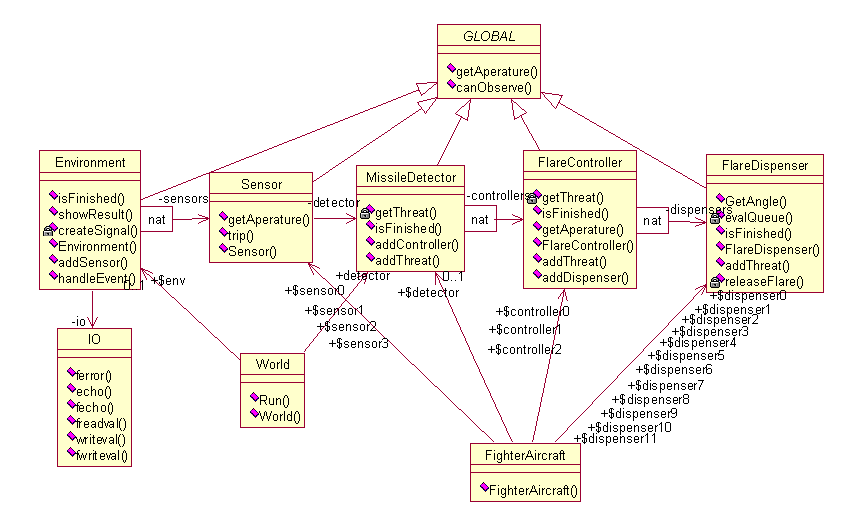
\includegraphics[width=6in]{figures/viceCMclassdiag.png}
\end{center}
\caption{Class Diagram for the Real-Time Distributed Counter Measures Model\label{fig:classdiagvice}}
\end{figure}

\subsection{Updating the Counter Measures Class}

As explained above the \texttt{CM} class have a number of new instance 
variables. The experimental hardware architecture considered here consists
of six \texttt{CPU}'s and three \texttt{BUS}'es. The declaration of these looks
like: 

\begin{lstlisting}
instance variables
cpu1 : CPU := new CPU (<FCFS>,1E6);
cpu2 : CPU := new CPU (<FCFS>,1E6);
cpu3 : CPU := new CPU (<FP>,1E9);
cpu4 : CPU := new CPU (<FCFS>,1E6);
cpu5 : CPU := new CPU (<FCFS>,1E6);
cpu6 : CPU := new CPU (<FCFS>,1E6);
bus1 : BUS := new BUS (<FCFS>,1E6,{cpu1,cpu3});
bus2 : BUS := new BUS (<FCFS>,1E6,{cpu2,cpu3});
bus3 : BUS := new BUS (<FCFS>,1E6,{cpu3,cpu4,cpu5,cpu6});
\end{lstlisting}

A graphical overview of this hardware architecture can be automatically
produced using the \showtrace\ feature from Overture. For this rather complex
architecture it looks as shown in Figure~\ref{fig:cpuarchitecture}.

\begin{figure}
\begin{center}
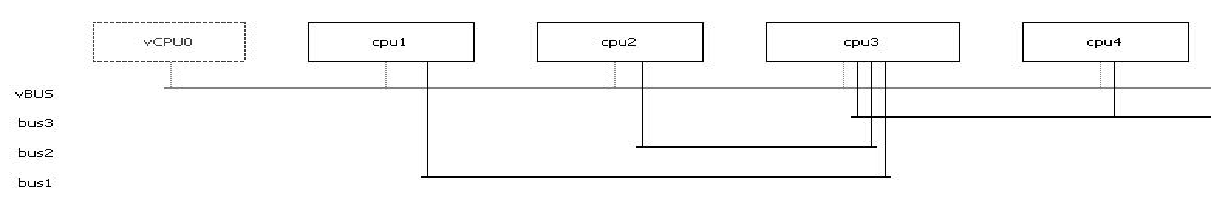
\includegraphics[width=\textwidth]{figures/cpuarchitecture.png}
\end{center}
\caption{CPU Architecture for the Distributed Counter Measures Model
\label{fig:cpuarchitecture}}
\end{figure}

The \texttt{CM} constructor then deploys all static instances to these
different \texttt{CPU}'s and set priorities for a number of the operations
used at the different \texttt{CPU}'s.

\begin{lstlisting}
operations

public CM: () ==> CM
CM () ==
  (cpu3.deploy(detector);
   cpu3.setPriority(MissileDetector`addThreat,100);
   cpu1.deploy(sensor0);
   cpu1.setPriority(Sensor`trip,100);
   cpu1.deploy(sensor1);
   cpu2.deploy(sensor2);
   cpu2.setPriority(Sensor`trip,100);
   cpu2.deploy(sensor3);
   cpu3.deploy(controller0);
   cpu3.setPriority(FlareController`addThreat,80);
   cpu4.deploy(dispenser0);
   cpu4.setPriority(FlareDispenser`addThreat,100);
   cpu4.setPriority(FlareDispenser`evalQueue,80);
   cpu4.deploy(dispenser1);
   cpu4.deploy(dispenser2);
   cpu4.deploy(dispenser3);
   cpu3.deploy(controller1);
   cpu5.deploy(dispenser4);
   cpu5.setPriority(FlareDispenser`addThreat,100);
   cpu5.setPriority(FlareDispenser`evalQueue,80);
   cpu5.deploy(dispenser5);
   cpu5.deploy(dispenser6);
   cpu5.deploy(dispenser7);
   cpu3.deploy(controller2);
   cpu6.deploy(dispenser8);
   cpu6.setPriority(FlareDispenser`addThreat,100);
   cpu6.setPriority(FlareDispenser`evalQueue,80);
   cpu6.deploy(dispenser9);
   cpu6.deploy(dispenser10);
   cpu6.deploy(dispenser11);
   )
\end{lstlisting}

\subsection{Updating the BaseRTThread Class}

The \texttt{BaseThread} class used in the concurrent VDM++ model is updated to encompass real-time information. This updated class is called \texttt{BaseRTThread}.

\begin{lstlisting}
class BaseRTThread

types

public static ThreadDef ::
  p : nat1
  isP : bool
  j : nat
  d : nat
  o : nat;
	
instance variables

protected period : nat1 := 1000E6;
protected isPeriodic : bool := true;
protected jitter : nat := 0;
protected delay : nat := 0;
protected offset : nat := 0;
\end{lstlisting}

The \texttt{ThreadDef} has added parameters for \emph{jitter}, \emph{delay} and \emph{offset}. Additional instance variables for holding values for these real-time parameters have also been added.

The \texttt{thread} section of the class has also been updated using the {\bf\ttfamily{periodic}} definition of threads using the real-time parameters defined above.

\begin{lstlisting}
thread
  periodic(period, jitter, delay, offset)(Step);
\end{lstlisting}

This has the unfortunate side-effect that the real-time framework described here does not support non-periodic threads. If non-periodic threads are needed in a real-time model, this can be done by specifying the non-periodic behaviour in the {\bf\ttfamily{thread}} section, and explicitly starting the non-periodic thread class using the {\bf\ttfamily{start}} keyword.

An example of the use of these added real-time parameters can be seen in the \texttt{CM} system class.

\begin{lstlisting}
system CM

instance variables

public static dispenser0 : FlareDispenser := new FlareDispenser(0, 
                           mk_BaseRTThread`ThreadDef(1000E6,true,0,0,0));
\end{lstlisting}

\subsection{Updating the RTTimeStamp Class}

The \texttt{TimeStamp} has been simplified since periodic threads are supported using the {\bf\ttfamily{periodic}} keyword, and hence threads does not need to be explicitly put to sleep and awoken. This means that the operations \texttt{WaitRelative}, \texttt{WaitAbsolute}, \texttt{BarrierReached}, \texttt{AddToWakeUpMap}, \texttt{NotifyThread}, \texttt{GetTime}and \texttt{ThreadDone} all have been removed from the class. The main difference is in the {\bf\ttfamily{sync}} section, where less operations have to be synchronised. This simplified class is called \texttt{RTTimeStamp}.

\begin{lstlisting}
sync 
  mutex (RegisterThread);
  mutex (UnRegisterThread); 
  mutex (RegisterThread, UnRegisterThread);
  mutex (IsInitialising);
  mutex (DoneInitialising);
\end{lstlisting}


\subsection{Updating the World Class}

The only change in the \texttt{World} class is the addition of additional parameters in instantiation of the \texttt{Environment} class.

\begin{lstlisting}
public World: () ==> World
World () ==
   env := new Environment("scenario.txt", 
              mk_BaseRTThread`ThreadDef(1000E6,true,10,900,0));
\end{lstlisting}

\subsection{Updating the Environment Class}

The constructor of the \texttt{Environment} has been updated. All active classes now inherit from \texttt{BaseRTThread}, and parameters for \emph{jitter}, \emph{delay} and \emph{offset} can also be passed in the constructor. Just like in the concurrent model, all active threads must pass a reference to the superclass \texttt{BaseRTThread} to ensure that all threads are registered correctly.

\begin{lstlisting}
class Environment is subclass of GLOBAL, BaseRTThread

operations

public Environment: seq of char * [ThreadDef] ==> Environment
Environment (fname, tDef) ==
 (def mk_ (-,input) = io.freadval[seq of inline](fname) in
    inlines := input;
   
  if tDef <> nil
  then (period := tDef.p;
        jitter := tDef.j;
        delay := tDef.d;
        offset := tDef.o;
       ); 
   BaseRTThread(self);
 );
\end{lstlisting}

Instead of using the \texttt{timerRef} reference the
\texttt{Environment} class now makes use of the special {\bf\ttfamily{time}}
keyword. This can for example be seen in the operation
\texttt{createSignal} where a {\bf\ttfamily{duration}} statement also has
been introduced.

\begin{lstlisting}
private createSignal: () ==> ()
createSignal () ==
  duration (10) 
  (if len inlines > 0
   then (dcl curtime : Time := time, done : bool := false;
         while not done do
           def mk_ (eventid, pmt, pa, pt) = hd inlines in
             if pt <= curtime
             then (for all id in set dom ranges do
                     def mk_(papplhs,pappsize) = ranges(id) in
                       if canObserve(pa,papplhs,pappsize)
                       then sensors(id).trip(eventid,pmt,pa);
                   inlines := tl inlines;
                   done := len inlines = 0)
             else done := true)
   else busy := false);
\end{lstlisting}

%Except for this the only difference for the new \texttt{Environment} class
%is that the thread is made periodic:

%\begin{lstlisting}
%thread

%periodic (1000,10,900,0) (createSignal)
%\end{lstlisting}

\subsection{Updating the Sensor Class}

The only change necessary for the \texttt{Sensor} class is that the 
\texttt{trip} operation is made asynchronous and the use of the 
{\bf\ttfamily{time}} keyword instead of the \texttt{World`timerRef.GetTime()} 
expression. Thus, now the \texttt{trip} operation looks like:

\begin{lstlisting}
async public trip: MissileType * Angle ==> ()
trip (pmt, pa) ==
  -- log and time stamp the observed threat
  detector.addThreat(pmt,pa,time)
pre canObserve(pa, aperture, SENSOR_APERTURE)
\end{lstlisting}

\subsection{Updating the Missile Detector Class}

The only update necessary for the \texttt{MissileDetector} class is that
the \texttt{addThreat} operation is made asynchronous.

\subsection{Updating the Flare Controller Class}

Just like for the \texttt{MissileDetector} class the only update
necessary for the \texttt{FlareController} class is that the
\texttt{addThreat} operation is made asynchronous.

\subsection{Updating the Flare Dispenser Class}

In the \texttt{FlareDispenser} class the \texttt{addThreat} and the 
\texttt{evalQueue} operations are made asynchronous. In addition, as
for a few other classes above there is now a reference to the 
{\bf\ttfamily{time}} keyword directly. Thus, these two operations now look
like:

\begin{lstlisting}
async public addThreat: EventId * MissileType * Time ==> ()
addThreat (evid, pmt, ptime) ==
  if missilePriority(pmt) > curprio
  then (dcl newplan : Plan :=  [],
            newtime : Time := ptime;
        -- construct an absolute time plan
        for mk_(fltp, fltime) in responseDB(pmt) do
          (newplan := newplan ^ [mk_ (fltp, newtime)];
           newtime := newtime + fltime );
        -- immediately release the first action
        def mk_(fltp, fltime) = hd newplan in
          releaseFlare(evid,fltp,fltime,time);
        -- store the rest of the plan
        curplan := tl newplan;
        eventid := evid;
        curprio := missilePriority(pmt);
        busy := true )
pre pmt in set dom missilePriority and
    pmt in set dom responseDB;

async evalQueue: () ==> ()
evalQueue () ==
  duration (10)
  (if len curplan > 0
   then (dcl curtime : Time := time, done : bool := false;
         while not done do
           (dcl first : PlanStep := hd curplan,
                next : Plan := tl curplan;
            let mk_(fltp, fltime) = first in
              if fltime <= curtime
              then (releaseFlare(eventid,fltp,fltime,curtime);
                    curplan := next;
                    if len next = 0
                    then (curprio := 0; 
                          done := true; 
                          busy := false ) )
              else done := true ) ) );
\end{lstlisting}

%In addition the thread is made periodic just like for the 
%\texttt{Environment} class.

%\begin{lstlisting}

%thread

%periodic (1000,0,0,0) (evalQueue)
%\end{lstlisting}

\subsection{Validation of the Model}

As for the VDM models presented earlier there is a need to
validate the correct behaviour of the real-time and distributed 
VDM-RT model presented
above. Both of these models use the standard
\texttt{IO} class for input and output. As previously one would start 
this by providing simple test cases and then gradually make them more
and more complex. Since the input format used for the real-time and
distributed VDM-RT model is identical to the one used for the
concurrent VDM++ model all the test cases with different
\texttt{scenario.txt} files can be reused again without any changes.
However, due to the timing now being closer to the ``real-world''
implementation of this system one needs to expect that the timing of
the output is not identical to what was in the previous model. It is
then up to the specifier to judge whether the timings give raise to
any kinds of bottlenecks. Once again the issue with the relative
angles for the
\texttt{FlareDispenser}'s are still present so the interested reader
can do the same kind of update to this model.

As for the previous VDM++ models the electronic
version of this model available on the web there is a rather complex 
\texttt{scenario.txt} that is sufficient to ensure that all parts of the
model have been exercised at least once just by interpreting
\texttt{new World().Run()}. Again is this documented using the test
coverage feature from Overture.

\subsection{Summary}

In this section we have presented a model of the counter measures
system that incorporates timing information and provides a distributed
architecture. It should be pointed out that to some extent this model
is still an idealization of the real world. Our model is deterministic and
assumes hardware performs perfectly and responds within specified
intervals, The model also takes quite a restricted view of what
external events may occur. These are not serious flaws in the proposed
approach for two reasons:

\begin{itemize}
\item Many of the assumptions made e.g.\ concerning determinism and
hardware behaviour are also made during host integration testing;
the behaviour of the system when these assumptions are broken could
only be tested during target integration testing.
\item It is in principal possible to model all manner of events. In
particular an ``unknown'' event could be modelled, and the system
behaviour described in the presence of such events.
\end{itemize}

However, it is worthwhile noting that work is undergoing to
incorporate the appropriate handling of faulty behaviour in the
environment is carried out in the DESTECS project~\cite{Broenink&10,Fitzgerald&10b,Fitzgerald&13a,Fitzgerald&13b}. 

\chapter{Synchronization}\label{chap:sync}

In this chapter issues relating to synchronization of concurrent
threads are addressed.  In particular the primitives for specifying
synchronous access to shared objects are described, and further
synchronization mechanisms that build on these primitives are also
given.

\section{Synchronization Primitives}

Synchronization in VDM++ is performed using \emph{permission predicates}. A
permission predicate is an expression specifying the circumstances in
which an operation may be executed.

\begin{lstlisting}
per !\emph{operation name}! => !\emph{guard condition}!
\end{lstlisting}

The semantics of a permission predicate is that when a client requests
an operation call, that operation's permission predicate is
evaluated. If it is true, execution may proceed and the operation may
be activated; if it is false, the client is blocked and the scheduler
is invoked.

Permission predicates are listed in the sync section of a class. As a
convenient abbreviation, the keyword \texttt{mutex} may be used to represent
mutual exclusion between operations. This is described in more detail
below, together with the different kinds of guard conditions.

A guard condition has scope over the instance variables of the
class. For example, consider the following specification of a
one-place buffer:
%\newpage

\begin{multicols}{2}
\begin{lstlisting}
class Buffer

instance variables
  data : [nat] := nil

operations
  public Put : nat ==> ()
  Put(v) == data := v;

sync
  per Put => data = nil;
\end{lstlisting}
\begin{lstlisting}
  public Get : () ==> nat
  Get() ==
   let n = data in
     (data := nil;
      return n)
  pre data <> nil

sync
  per Get => data <> nil

end Buffer
\end{lstlisting}
\end{multicols}

\subsection{History Counters}

A guard condition is also allowed to refer to \emph{history counters}. These
describe the history of a particular operation. There are three basic
history counters:

\begin{description}
\item[\texttt{\#req(op)}] The number of times op has been requested in
a particular object;
\item[\texttt{\#act(op)}] The number of times op has been activated in
a particular object;
\item[\texttt{\#fin(op)}] The number of times op has completed
execution in a particular object.
\end{description}

As a simple example, consider an N-place buffer:
%\newpage

\begin{multicols}{2}
\begin{lstlisting}
class BufferN

values
  N : nat = 5

instance variables

  data : seq of nat := [];
  inv len data <= N

operations
  public Put : nat ==> ()
  Put(v) ==
    data := data ^ [v];

\end{lstlisting}
\begin{lstlisting}
  public Get : () ==> nat
  Get() ==
    let n = hd data in
      (data := tl data;
       return n)
  pre data <> []

sync
  per Put =>
    #fin(Put) - #fin(Get) < N;
  per Get =>
    #fin(Get) < #fin(Put);

end BufferN
\end{lstlisting}
\end{multicols}

Note that in this example the permission predicates could have been
equally well expressed in terms of the class's instance
variables. However, in general, use of such guards allows more
sophisticated synchronization predicates. For example we can express
the requirement that only N invocations of \texttt{Put} may be active at any
time:

\begin{lstlisting}
per Put => #fin(Put) - #fin(Get) < N and #fin(Put) = #act(Put);
\end{lstlisting}

In addition to the basic history counters, two derived history counters exist:

\begin{description}
\item[\texttt{\#active(op)}] The number of currently active instances
of op.  So \\ {\bf\ttfamily{\#active}}\texttt{(op) = }{\bf\ttfamily{\#act}}\texttt{(op) - }{\bf\ttfamily{\#fin}}\texttt{(op)}.
\item[\texttt{\# waiting(op)}] The number of non-activated requests for
op.  So \\ {\bf\ttfamily{\#waiting}}\texttt{(op) = }{\bf\ttfamily{\#req}}\texttt{(op) - }{\bf\ttfamily{\#act}}\texttt{(op)}.
\end{description}

\subsection{Mutex}

It is possible to specify mutual exclusion (\emph{mutex}) between operation
invocations using the basic history counters. However it is such a
common requirement that the keyword {\bf\ttfamily{mutex}} may be used as shorthand for
a {\bf\ttfamily{mutex}} predicate.

A {\bf\ttfamily{mutex}} predicate allows the user to specify either
that all operations of the class are to be executed mutually
exclusive, or that a list of operations are to be executed mutually
exclusive to each other. Operations that appear in one mutex predicate
are allowed to appear in other {\bf\ttfamily{mutex}} predicates as
well, and may also be used in the usual permission predicates. Each
{\bf\ttfamily{mutex}} predicate will implicitly be translated to
permission predicates using history guards for each operation
mentioned in the name list. For instance,

\begin{lstlisting}
sync
  mutex(opA, opB);
  mutex(opB, opC, opD);
  per opD => someVariable > 42;
\end{lstlisting}

\noindent
would be translated to the following permission predicates (which are
semantically equivalent to the above expression):

\begin{lstlisting}
sync
  per opA => #active(opB) = 0;
  per opB => #active(opA) = 0 and
             #active(opC) + #active(opD) = 0;
  per opC => #active(opB) + #active(opD) = 0;
  per opD => #active(opB) + #active(opC) = 0 and
             someVariable > 42;
\end{lstlisting}

Note that it is only permitted to have one explicit permission predicate for
each operation in each class.

A {\bf\ttfamily{mutex(all)}} constraint specifies that all of the operations
specified in that class \emph{and any superclasses} are to be executed
mutually exclusively.

It is clear that using {\bf\ttfamily{mutex}}, concurrent execution of critical regions
can be prevented.

\section{Wait-Notify}\label{sec:waitnotify}

A popular synchronization mechanism is the wait-notify used in the
Java programming language \cite{Gosling&00}. To understand this
concept, consider two threads \texttt{Producer} and 
\texttt{Consumer} which communicate
by an unsynchronized shared buffer, \texttt{b} as defined below:

\begin{multicols}{2}
\begin{lstlisting}
class UnsyncBuffer

instance variables
  data : [nat] := nil

operations
  public Put : nat ==> ()
  Put(v) ==
    data := v;
\end{lstlisting}
\begin{lstlisting}

  public Get : () ==> nat
  Get() ==
    let n = data in
      (data := nil;
       return n)
  pre data <> nil

end UnsyncBuffer
\end{lstlisting}
\end{multicols}

The unsynchronized buffer is used to communicate data between the producer and
consumer threads.

\begin{multicols}{2}
\begin{lstlisting}
-- Producer thread
while true do
  (let v = Produce() in
     b.Put(v))
\end{lstlisting}
\begin{lstlisting}

-- Consumer thread
while true do
  Consume(b.Get())
\end{lstlisting}
\end{multicols}

Of course the problem that arises is that when the consumer thread
consumes data, there need not necessarily be any valid data in the
buffer. Moreover, if the producer thread generates data ``too fast''
for the consumer, data could be lost.

A wait-notify object allows access to the buffer to be synchronized
across the two threads. Suppose \texttt{o} is a wait-notify object.

\begin{multicols}{2}
\begin{lstlisting}
-- Producer thread
while true do
  (let v = Produce() in
     b.Put(v)
   o.Notify();
   o.Wait())
\end{lstlisting}
\begin{lstlisting}

-- Consumer thread
while true do
  (o.Wait();
   Consume(b.Get());
   o.Notify())
\end{lstlisting}
\end{multicols}

Following a call to \texttt{o.Wait}, a thread blocks until another
thread calls \texttt{o.Notify}. Thus in this example we can see that
following production of a value, the producer thread places this in
the buffer, notifies the consumer thread and then blocks. The consumer
thread is blocked until it is notified by the producer thread; it then
consumes the data in the buffer, and afterwards notifies the producer
thread.

The advantage of using Wait-Notify is that it can be used to
synchronize access to an arbitrary shared object; that is, this shared
object need not have been designed with sharing in mind. This greatly
simplifies specification and design, as consideration of
synchronization can thus be safely postponed until design of the
dynamic architecture begins.

Care must be taken with the initialization of a wait-notify mechanism,
otherwise deadlocks can occur. For instance in the above example, if
the producer thread executes first, following its \texttt{notify} both
producer and consumer are waiting for a \texttt{notify}, so this must
be supplied externally. Alternatively the threads can be organized in
such a way as to force the consumer to be executed first.

%% Note that Wait-Notify is not a primitive in VDM++; instead it is a
%% user-defined class.  Its definition may be found in
%% Appendix~\ref{app:waitnotify}.

\section{Thread Completion}

A common use of permission predicates is to block the default thread
until all other threads have completed. For example, consider the
model in Figure~\ref{fig:notwait}.

When \texttt{Main} executes, it creates and starts an instance of
\texttt{SubThread}, but it delivers the contents of the shared object before
\texttt{SubThread} has necessarily had a chance to place any data in
it.

In order to overcome this problem, the shared object should be used to
determine completion. An operation \texttt{IsFinished} should be added
to the specification of \texttt{Shared}. Calls to this operation should block
until it is determined that \texttt{SubThread} has completed.

\begin{figure}
\begin{multicols}{2}
\begin{lstlisting}
class Shared

instance variables
  data : seq of nat := []

operations
  public Put : nat ==> ()
  Put(n) ==
    data := data ^ [n];

  public Get : () ==>
               seq of nat
  Get() == return data

sync

mutex(Put);
mutex(Put,Get)

end Shared

class SubThread

instance variables
  s : Shared

operations
\end{lstlisting}
\begin{lstlisting}

  public Init : Shared ==> ()
  Init(ns) == s := ns

thread
  for i = 1 to 100 do
    s.Put(i * i)

end SubThread

class MainThread

operations

  public Main :
           () ==> seq of nat
  Main() ==
    (dcl s : Shared :=
               new Shared(),
         t : SubThread :=
               new SubThread();
     t.Init(s);
     start(t);
     return s.Get() 
    )

end MainThread
\end{lstlisting}
\end{multicols}
\caption{Not Waiting For Thread Completion\label{fig:notwait}}
\end{figure}

The specification for operation \texttt{Main} would then be:

\begin{lstlisting}
public Main : () ==> seq of nat
Main() ==
  ( dcl s : Shared := new Shared(),
        t : SubThread := new SubThread();
    t.Init(s);
    start(t);
    s.IsFinished();
    return s.Get()
  )
\end{lstlisting}

The determination of thread completion can be achieved implicitly or
explicitly. The implicit approach is based on the amount of data
generated by the thread. For instance if it is known that the thread
will generate 100 values, this can be used to determine completion:

\begin{multicols}{2}
\begin{lstlisting}
class Shared

instance variables
  data : seq of nat := []

operations
  public Put : nat ==> ()
  Put(n) ==
    data := data ^ [n];

  public Get :
          () ==> seq of nat
  Get() == return data;
\end{lstlisting}
\begin{lstlisting}

  public IsFinished :
            () ==> ()
  IsFinished() == skip;

sync

mutex(Put);
mutex(Put,Get);
per IsFinished =>
    #fin(Put) = 100

end Shared
\end{lstlisting}
\end{multicols}

In the explicit approach, the thread which is being waited on informs
the shared object of its completion:
%\newpage

\begin{multicols}{2}
\begin{lstlisting}
class Shared

instance variables

  data : seq of nat := [];
  finished : bool := false;

operations

  public Put : nat ==> ()
  Put(n) == data := data ^ [n];

  public Get :
          () ==> seq of nat
  Get() == return data;

\end{lstlisting}
\begin{lstlisting}
  public IsFinished :
           () ==> ()
  IsFinished() == skip;

  public Finished : () ==> ()
  Finished() ==
    finished := true

sync
  mutex(Put);
  mutex(Put,Get);
  mutex(Finished);
  per IsFinished => finished

end Shared
\end{lstlisting}
\end{multicols}

\section{Summary}

In this chapter difference mechanisms for synchronization have been
presented: synchronization primitives using permission predicates, and
the Wait-Notify mechanism.  In general synchronization based on
permission predicates can be extremely powerful, as such predicates
are highly expressive. The price of this power is that it can be very
difficult to debug models suffering from deadlocks if such permission
predicates are used. Therefore it is recommended that wherever
possible the wait-notify mechanism is used, as it is easy to
debug\footnote{Alternatively the trace file produced by Overture or \vdmtools\
can be used to get insight into problems such as deadlocks.}
breakpoints can be placed within the operations of the wait-notify
class to help identify any problems.


\chapter{Periodicity}\label{chap:period}

Many real-time systems have an element of periodicity -- something
which repeats with fixed frequency. In this chapter we describe how
periodicity can be modelled.

\section{Periodic Threads}\label{sec:periodthread}

Threads may be periodic: that is, an operation can be called with
fixed frequency. A typical use of this is to poll an external sensor.

\begin{lstlisting}
class Sensor

operations
  public GetData : () ==> nat
  GetData() ==
    is not yet specified

end Sensor

class SensorPoll

instance variables
  lastReading : [nat] := nil;
  sensor : Sensor

operations
  public Init : Sensor ==> ()
  Init(ns) ==
    sensor := ns;

  PollSensor : () ==> ()
  PollSensor() ==
    lastReading :=
       sensor.GetData()

thread
  periodic (100,10,90,0) (PollSensor)

end SensorPoll

class Main

operations
  public Run : () ==> ()
  Run() ==
  ( dcl sp : SensorPoll :=
              new SensorPoll(),
        s : Sensor := new Sensor();
    sp.Init(s);
    start(sp)
  )

end Main
\end{lstlisting}

Here the sensor thread \texttt{sp} will execute approximately 
every 100 time units (1 time unit = 1 nanosecond)
following execution of the statement {\bf\ttfamily{start}}\texttt{(sp)}.

Note that in a simple system such as the one above,
\texttt{PollSensor} will be invoked approximately every 100 time
units. The second parameter to the periodic statement indicates that a
jitter of up to 10 time units can be allowed for the periodic invocation of this
thread. The third parameter indicates that there is going to be at
least 90 time units between two instances of this periodic
thread. Finally, the last parameter indicates that no offset is
required for the invocation of this periodic thread. This is a feature
that is most valuable if a number of threads are started at the same
time, and there is a desire to carry them out in a special order.

In systems with more threads, the periodicity merely
informs the scheduler when a particular periodic thread is
schedulable. Thus in practice it is possible for periodic threads to
be delayed. In fact, it is often an interesting property of a model
that periodic threads are being delayed, as it could indicate that
portions of the model need to be redesigned. Therefore in the time
trace file a special event is output if a periodic thread is delayed.

\subsection{Periodic Threads and Scheduling}

Periodic threads are subject to the same scheduling policy as other
threads. This has a number of implications for their
use. Specifically:

\begin{itemize}
\item Even if a periodic thread which has not
completed by the end of its period another periodic thread will be
made possible at the next period. Thus it is possible to multiple
invocations of a periodic thread at the same time. However, as a user
one should be careful about such usage, since it means that an
increasing number of threads may be produced.
\item Under priority-based scheduling, a periodic thread could miss
its deadline because a higher priority thread has been scheduled.
\end{itemize}

\section{Modelling Periodic Events}\label{sec:modperevents}

Typically, an external event is modelled as an operation
invocation. Thus to model a periodic event, it should be modelled as a
periodic operation invocation. For example, suppose we wish to model a
clock:

\begin{lstlisting}
class Clock

instance variables
  curtime : nat := 0

operations
  public GetTime : () ==> nat
  GetTime() == return curtime;

  Tick : () ==> ()
  Tick() == curtime := curtime + 1

thread
  periodic (100,0,0,0)(Tick)

end Clock
\end{lstlisting}

An instance of \texttt{Clock} has a thread which will be executed
every 100 time units. Such a clock could be shared amongst several
threads, and used to synchronize behaviour across the sharing threads. 
Other examples of timers can be found in Section~\ref{sec:timerclass} and 
in Appendix~\ref{sec:TimeStamp}.

\section{Statically Schedulable Systems}

Systems which are known to be statically schedulable with specific
periods can be simply modelled using periodic threads. For example
suppose that we have a system with three threads \texttt{A},
\texttt{B} and \texttt{C}, which have frequencies 30, 70 and 110 time
units respectively.

\begin{lstlisting}
class A
...
thread
  periodic (30,0,0,0) (OpA)
end A

class B
...
thread
  periodic (70,0,0,0) (OpB)
end B

class C
...
thread
  periodic (110,0,0,0) (OpC)
end C

class Main

operations
  public Run : () ==> ()
  Run() ==
  ( dcl a : A := new A(),
        b : B := new B(),
        c : C := new C();
    ...
    startlist({a,b,c});
    ...
  )
end Main
\end{lstlisting}

In case it was desirable to let one of them start later 
than the others it would be possible to set the offset to a positive
value for that one.

\section{Summary}

Systems exhibiting periodicity can be described using VDM in a
straightforward manner, using language primitives. Based on these
primitives, features such as timers and clocks can be built into
models.

Note that in general, if a system is statically schedulable and does
not have high CPU utilization requirements, then rate monotonic
analysis \cite{Audsley&93,Burns95} may be used to schedule the system. In
this case the problems of meeting deadlines etc are automatically
resolved, so for such systems rate monotonic analysis is preferable.

%\fbox{More examples with offset should be introduced!!!!}

\chapter{Scheduling Policies} \label{chap:schedule}

Overture and \vdmtools\ supports a number of different scheduling
policies. In this chapter we describe these various policies, and
summarize the implications for the model of each particular policy.

At any point during execution Overture and \vdmtools\ employs two
complementary scheduling policies: the primary scheduling policy and
secondary scheduling policy.

The primary scheduling policy determines when a thread should be
descheduled. The secondary scheduling policy determines the order in
which the scheduler tries to find the next thread to schedule. We
consider each category separately.

\section{Primary Scheduling Algorithm}

Overture and \vdmtools\ offers a choice of primary scheduling algorithm
between time limited and cooperative. In general, a thread executes
until an operation call is made, for which the permission predicate is
false, at which point the thread blocks.

In a cooperative scheduling algorithm, there is no other way in which
a thread may be descheduled: each thread is allowed to run to
completion.

In a time limited scheduling algorithm no thread is allowed to execute
continuously for more than some defined period; when this period is
complete the scheduler will deschedule the thread.

Two time limited scheduling algorithms are available:
\emph{instruction number scheduling} and \emph{time slice
scheduling}. Under instruction number scheduling the amount of time
each thread executes for is limited by the number of instructions
executed during execution of the thread. Thus under instruction number
scheduling, the decisions made by the scheduler are independent of
duration statements or the default cycles information.  Under time
slice scheduling, the amount of time each thread executes for is
limited by a fixed amount of simulated time. Thus under this
scheduling algorithm the amount of time each thread executes for is
affected by duration statements, and also by the default duration
information.

\section{Secondary Scheduling Algorithm}

Two secondary scheduling algorithms are supported: round-robin or
priority-based.

\subsection{Round-Robin Scheduling}

Under round-robin, the scheduler uses an arbitrary, fixed order in
which to find the next thread to execute. Consider the following
example. Suppose we have threads \texttt{t1}, \texttt{t2} and
\texttt{t3}, and that the order that the scheduler uses is
\texttt{[t1,t2,t3]}. Suppose further that \texttt{t1} is descheduled
and at this point \texttt{t2} is blocked, and \texttt{t3} is
schedulable.

The scheduler would first test whether \texttt{t2} is schedulable;
since it is blocked, it would then check whether \texttt{t3} is
schedulable. Thus \texttt{t3} would be scheduled.  

Suppose now that when \texttt{t3} is descheduled, \texttt{t1} and
\texttt{t2} are both schedulable. The scheduler would first check
\texttt{t1}, and since this is schedulable, it would be selected and
executed.

Thus under round-robin scheduling a weak fairness property exists
\cite{Lamport91}: a thread that is never blocked will eventually be
scheduled.

\subsection{Priority-based Scheduling}

Priority-based scheduling is a variant on round-robin scheduling. A
numeric priority is assigned to each thread. When the scheduler needs
to select the next thread to be scheduled, all the highest priority
threads are checked using a standard round-robin; if no schedulable
thread is found, then all threads of the second-highest priority are
checked using a standard round-robin, and so on.

To illustrate this, consider the following example. Suppose we have
threads \texttt{a1}, \texttt{a2}, \texttt{a3}, \texttt{b1},
\texttt{c1} and \texttt{c2}. Threads \texttt{a1}, \texttt{a2} and
\texttt{a3} have priority 3; \texttt{b1} has priority 2 and
\texttt{c1} and \texttt{c2} have priority 1. Suppose that the
round-robin orders used are:

\begin{tabular}{cl}
Priority & Order \\ \hline
3        & \texttt{[a1,a2,a3]} \\
2        & \texttt{[b1]} \\
1        & \texttt{[c1, c2]} \\
\end{tabular}

Consider scheduling in the following situation:

\begin{tabular}{cl}
Thread & Status \\ \hline
a1 & Blocked \\
a2 & Schedulable \\
a3 & Schedulable \\
b1 & Schedulable \\
c1 & Schedulable \\
c2 & Schedulable \\
\end{tabular}

The scheduler examines the highest priority threads first. Thus first
thread \texttt{a1} would be checked; it is blocked so \texttt{a2}
would be checked. Since \texttt{a2} is schedulable it would be
selected.

Now consider another situation:

\begin{tabular}{cl}
Thread & Status \\ \hline
a1 & Blocked \\
a2 & Blocked \\
a3 & Blocked\\
b1 & Blocked\\
c1 & Blocked\\
c2 & Schedulable\\
\end{tabular}

The scheduler examines threads of priority 3 first; they are all
blocked. It then examines threads of priority 2; they are also all
blocked. Finally it examines threads of priority 1: first \texttt{c1}
is checked, but it is blocked, then \texttt{c2} is checked. Since \texttt{c2}
is schedulable it is selected.

Note that for threads which are not of the highest priority, there are no fairness properties: it is possible for them to starve.

\subsection{Priority of Default Thread}

Consider the following model shown in Figure~\ref{fig:priodefault}

Suppose that in the Overture or \vdmtools\ interpreter
the expression \texttt{new B().Main()} is executed
using round-robin scheduling. The model will then execute, and a
result will be delivered consisting of a sequence with at least 11
elements. The thread initiated by issuing a command in the interpreter is
called the default thread.

Consider now the situation in which the model is executed using
priority-based scheduling, where \texttt{A} has priority 2, and
\texttt{B} has priority 1. In this case the computation will never
terminate, since \texttt{B} will never be scheduled due to having a
lower priority than \texttt{A}, which is always schedulable.

\begin{figure}
\begin{lstlisting}
class A

instance variables
  data : seq of nat := []

operations
  public IsFinished:() ==> ()
  IsFinished() == skip;

  public Get: () ==>
              seq of nat
  Get() == return data

sync
  per IsFinished =>
      len data > 10

thread
  (dcl i : nat := 0;
   while true do
   ( data := data ^ [i];
     i := i + 1 ))

end A

class B

operations
  public Main:() ==> seq of nat
  Main() ==
  ( dcl a : A := new A();
    start(a);
    a.IsFinished();
    a.Get())

end B
\end{lstlisting}
\caption{Example illustrating the Priority of the Default Thread\label{fig:priodefault}}
\end{figure}

To avoid this problem, Overture and \vdmtools\ implements the following policy:
the default thread is always given a strictly higher priority than any
other thread in the system, regardless of what priority may actually
have been specified for the class from which the default thread is
derived. In this way the default thread is always checked first by the
scheduler.

\chapter{Time Trace Analysis}\label{chap:timetrace}

In this chapter we describe the format of the time trace files, and
the kinds of analysis that may be performed on them.

\section{Timed Trace Files}

The time trace files generated during execution contain information
about thread swapping, messages passed between CPUs and operation
requests, activations and completions.

\subsection{Example}

An extract from a trace file is shown below as an example in Figure~\ref{fig:examplelogfile}. 

\begin{figure}
{\small
\begin{alltt}
CPUdecl ->  id: 13 expl: false sys: "none" name: "vCPU 7"
DeployObj ->  objref: 160 clnm: "FlareDispenser" cpunm: 0 time: 728
OpRequest -> id: 1 opname: "FlareController`addDispenser" objref: 138 
             clnm: "FlareController" cpunm: 0 async: false time: 736
MessageRequest -> busid: 0 fromcpu: 0 tocpu: 9 msgid: 23 
                  callthr: 1 opname: "FlareController`addDispenser" 
                  objref: 138 size: 80 time: 736
MessageActivate -> msgid: 23 time: 736
MessageCompleted -> msgid: 23 time: 736
ThreadSwapOut -> id: 15 objref: 152 clnm: "FlareDispenser" 
                 cpunm: 9 overhead: 2 time: 736
ThreadCreate -> id: 16 period: false objref: 138 
                clnm: "FlareController" cpunm: 9 time: 738
ThreadSwapIn -> id: 16 objref: 138 clnm: "FlareController" 
                cpunm: 9 overhead: 2 time: 738
\end{alltt}
}
\caption{Example extract from a \texttt{logfile}\label{fig:examplelogfile}}
\end{figure}

Each entry in the time trace file consists of an event name, and event
information, separated by \texttt{->}. Events fall into different
categories, object history events, message events, declaration events,
deployment events and thread events. The category
dictates the event information provided.

\begin{description}
\item[Object history events] consist of operation requests, activations and
completions. The information provided for such events are: the
operation called; information whether it is an asynchronous operation;
the object reference id and the \texttt{CPU} id on which the operation has
been called; the class which the object is an instance of; and the
time at which the event occurred.

\item[Message events] are similar to operation requests except that they
    identify requests, activations and completions of messages communicated
    over a \texttt{BUS}. These messages are automatically derived by 
    Overture when an operation is to be invoked on an instance that has been
    deployed to a different \texttt{CPU}. Each message is given a unique
    identification. Thus, it is only the message request events that contain
    all information about the \texttt{BUS} used, the \texttt{CPU} it is 
    coming from and to, etc. Importantly it also contains a size attribute
    that is derived from the values that are passed over as parameters for
    the operation to be called at the other \texttt{CPU}. 

\item[Declaration events] are included in system ``classes'' where
    it is possible to declare
    \texttt{CPU}'s and \texttt{BUS}'es. In addition \texttt{CPU}'s may be
    implicitly declared when new objects are created inside the \texttt{World}
    class and this is also logged.

\item[Deployment events] are logged whenever objects are created. 
     An object may initially be created and deployed at the virtual 
     \texttt{CPU} (always with cpuid 0) and then subsequently deployed
     at a different \texttt{CPU}.

\item[Thread events] correspond to a thread being created, killed,
swapped in or out, or (for
periodic threads) a thread which has missed its deadline being swapped
in. In this case the thread id is provided, together with the object
reference id for the object owning the thread, the class which the
object is an instance of, the time of the event, and (for delayed
periodic threads) the delay.
\end{description}

\section{Analysis Tools}

Since the time trace file quickly becomes large, it is essential to
use tools to analyze them. Here we give some examples of such
tools. 
%Tools may be generic or bespoke, that is they may produce
%general statistic concerning traces, or they may produce
%application-relevant information. However, most users will initially
%use a generic tool and only dedicate extra effort to making a bespoke
%solution when the generic tool is not capable of performing an especially
%desired analysis.

%\subsection{Generic Analysis Tools}

At the moment one external generic analysis tool for trace files produced by
Overture exists. This is the \showtrace\ feature from Overture.

The \showtrace\ feature is able to type check a trace file and if it 
is parsed and checked to be correct it is able to show:

\begin{itemize}
\item A system architecture with the \texttt{CPU}'s and the connecting
      \texttt{BUS}'es as shown in Figure~\ref{fig:cpuarchitecture}.
\item An execution overview the illustrates when the different 
      \texttt{CPU}'s and \texttt{BUS}'es are active (see 
      Figure~\ref{fig:exeoverview} for an example).
\item A detailed graphical overview for each \texttt{CPU} where the
      different objects that have been deployed to that \texttt{CPU} and
      the different threads executing are shown (see 
      Figure~\ref{fig:detailedexe} for an example).
\end{itemize}

\begin{figure}
\begin{center}
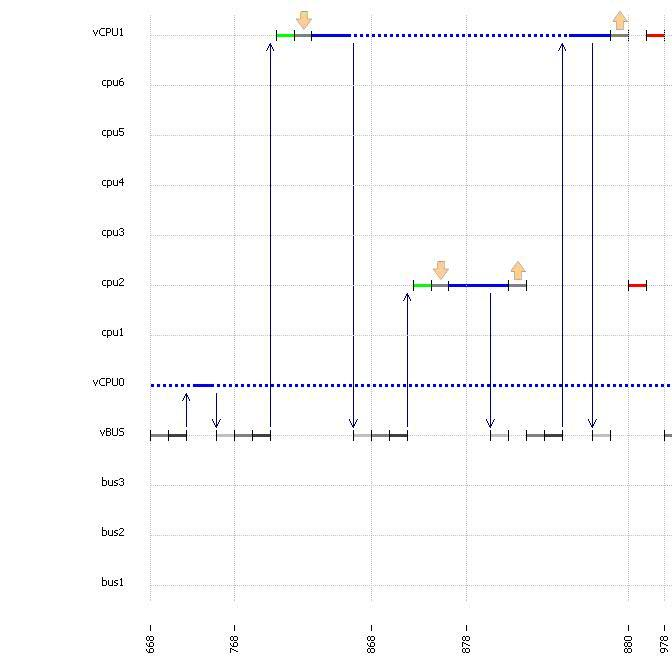
\includegraphics[width=\textwidth]{figures/exeoverview.png}
\end{center}
\caption{An extract from an execution overview for the counter measures example\label{fig:exeoverview}}
\end{figure}

\begin{figure}
\begin{center}
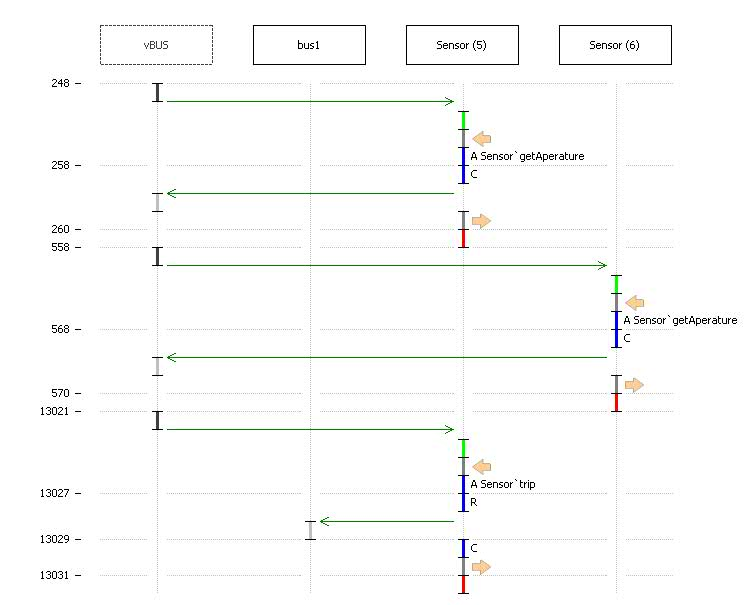
\includegraphics[width=5.5in]{figures/detailedexe.png}
\end{center}
\caption{An extract from one \texttt{CPU} execution for the counter measures example\label{fig:detailedexe}}
\end{figure}

%% \subsection{Bespoke Analysis Tools}

%% There are of course many different bespoke analysis tools which could
%% be developed for trace files, according to the application domain and
%% the real-time properties of interest.  Here we focus on a couple of
%% general approaches.

%% \subsubsection{Use of Standard Text-Processing Tools}

%% Since the time trace file is simply an ASCII file, manipulation of
%% such files is straight-forward (e.g.\ in Perl \cite{Wall&92}). An
%% example of this is a Perl script which is used to generate an Excel
%% spreadsheet from a trace file from an earlier version of the
%% missile counter measures model, as shown in
%% Figure~\ref{fig:chartExcel}. In this figure a graphical depiction of
%% the times at which the various threads in a model are active is
%% shown. Since standard office tools are able to accept comma separated
%% files, writing such a script is simply a matter of processing a stream
%% of data.

%% \subsubsection{Visualization}

%% A common bespoke analysis tool is a visualization of a trace,
%% superimposing the time at which particular events occur on the
%% activity lines of threads. An example of this is shown in
%% Figure~\ref{fig:vistrace}.

%% Given the preponderance of GUI toolkits such as Java Swing
%% \cite{JavaSwing}, Qt \cite{Qt} and Visual Basic \cite{VisualBasic},
%% such visualizations are relatively easy to develop, but certainly more
%% time consuming than using the \showtrace\ feature. Moreover they
%% can be extremely powerful in communicating the behaviour of a model to
%% a domain expert.

%% \begin{figure}
%% \begin{center}
%% 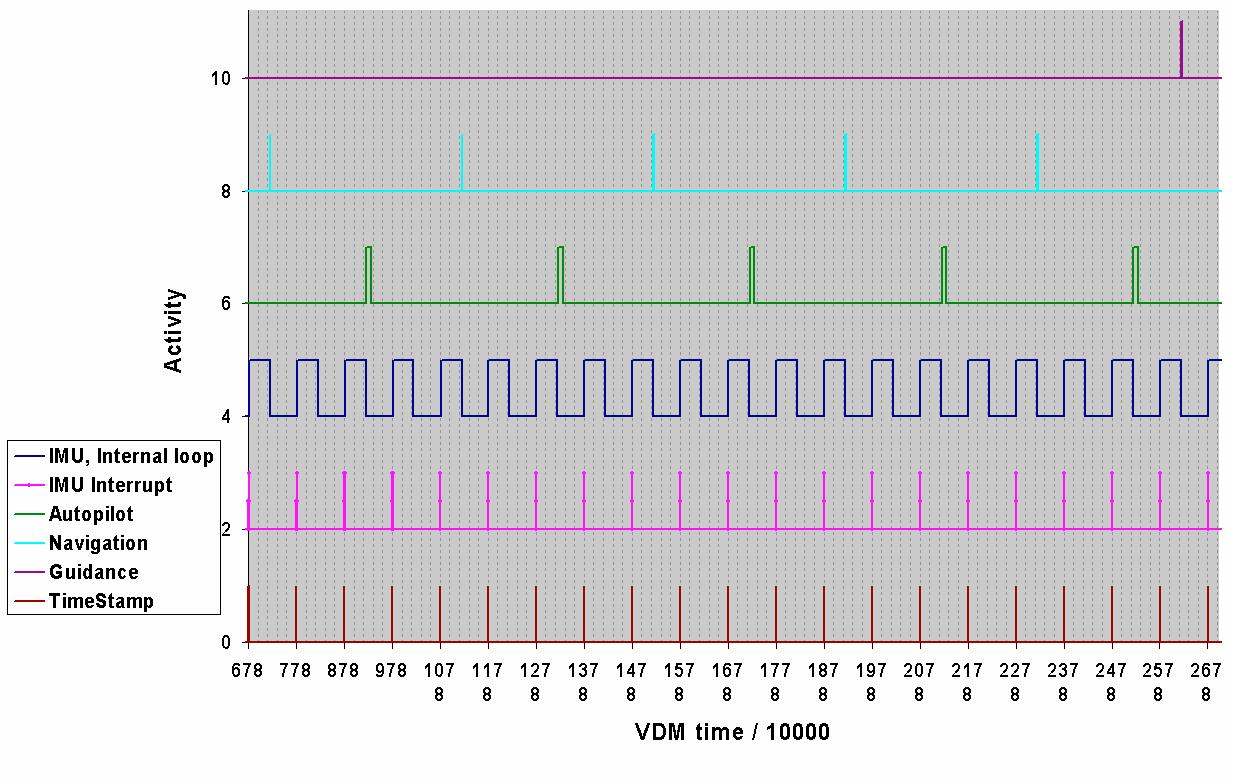
\includegraphics[width=\textwidth]{figures/analysismissile.jpg}
%% \end{center}
%% \caption{A chart in Microsoft Excel generated from a time trace file\label{fig:chartExcel}}
%% \end{figure}

%% \begin{figure}
%% \begin{center}
%% 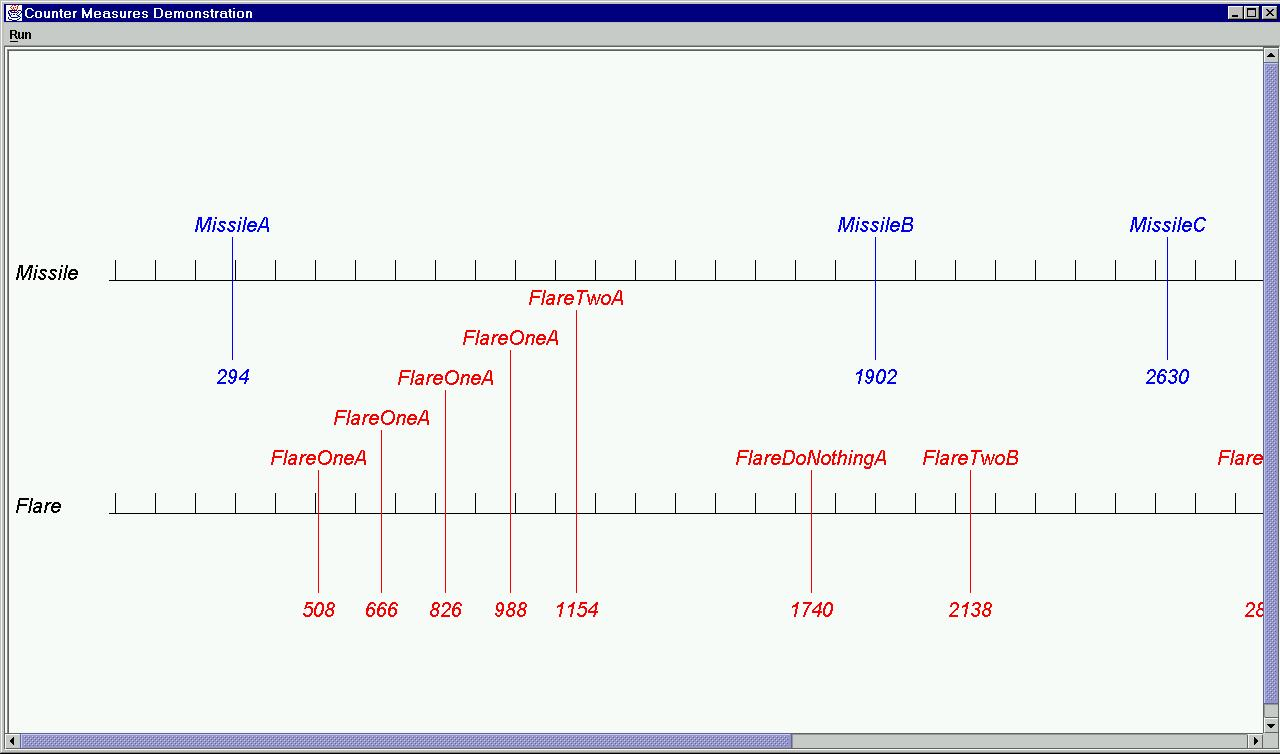
\includegraphics[width=\textwidth]{figures/bespokemissile.jpg}
%% \end{center}
%% \caption{Visualization of a time trace file\label{fig:vistrace}}
%% \end{figure}

\subsubsection{Timed Assertions}

The time trace file can be thought of as simply being a sequence. It
is therefore possible to specify VDM-SL predicates on such a sequence.

For this to be possible, an abstract VDM-SL representation of a trace
file is needed.  This is now described.

A number of types are defined to represent the different fields in a
time trace file. We represent a string as a sequence of characters,
and object references and thread ids as natural numbers.

\begin{lstlisting}
types

  String = seq of char;
  OBJ_Ref = nat;
  ThreadId = nat;
\end{lstlisting}

A trace is an ordered sequence of trace events.

\begin{lstlisting}
Trace = seq of TraceEvent
\end{lstlisting}

There are many different kinds of trace events:

\begin{lstlisting}
TraceEvent = 
     ThreadSwapIn | ThreadSwapOut | DelayedThreadSwapIn |
     OpRequest | OpActivate | OpCompleted | ThreadCreate |
     ThreadKill |  MessageRequest | MessageActivate |
     MessageCompleted | ReplyRequest | CPUdecl | BUSdecl |
     DeployObj; 
\end{lstlisting}

A thread swap in event consists of the id of the thread being swapped
in, the object reference owning the thread, the class name in
which the thread is defined, the cpu where it is running, the 
timing overhead of swapping in the thread and the time on that \texttt{CPU}.

\begin{lstlisting}
  ThreadSwapIn :: id       : ThreadId
                  objref   : [OBJ_Ref]
                  clnm     : String
                  cpunm    : nat 
                  overhead : nat
                  attime   : nat;
\end{lstlisting}

A delayed thread swap in has an extra field representing the delay.

\begin{lstlisting}
DelayedThreadSwapIn :: id       : ThreadId
                       objref   : [OBJ_Ref]
                       clnm     : String
                       delay    : real
                       cpunm    : nat
                       overhead : nat
                       attime   : nat;
\end{lstlisting}

A thread swap out contains the same information as a thread swap in.

\begin{lstlisting}
ThreadSwapOut :: id       : ThreadId
                 objref   : [OBJ_Ref]
                 clnm     : String
                 cpunm    : nat
                 overhead : nat
                 attime   : nat;
\end{lstlisting}

An operation request contains the thread in which the request was made,
the name of the operation, a reference
to the object on which the request occurred, the name of the class
which this object is an instance of, the cpu where it is running, the 
arguments to the operation (if a special user option is set for storing
this detailed level of information), whether it is an asynchronous operation
and finally the time on that \texttt{CPU}.

\begin{lstlisting}
OpRequest :: id     : ThreadId
             opname : String
             objref : OBJ_Ref
             clnm   : String
             cpunm  : nat
             args   : [seq of VAL]
             isasync: bool
             attime : nat;
\end{lstlisting}

Operation activations and completions contain part of the information as
operation requests (the result of the operation is only present if the 
user have explicitly asked to get this information logged).

\begin{lstlisting}
OpActivate :: id     : ThreadId
              opname : String
              objref : OBJ_Ref
              clnm   : String
              cpunm  : nat
              isasync: bool
              attime : nat;

OpCompleted :: id     : ThreadId
               opname : String
               objref : OBJ_Ref
               clnm   : String
               cpunm  : nat
               res    : [VAL]
               isasync: bool
               attime : nat;
\end{lstlisting}

Trace events are also present whenever threads are being created and killed
after completion. Note that the creating of a thread also contains information
whether it is a periodic thread.

\begin{lstlisting}
ThreadCreate :: id     : ThreadId
                period : bool
                objref : [OBJ_Ref]
                clnm   : [String] 
                cpunm  : nat
                attime : nat;

ThreadKill :: id    : ThreadId
              cpunm : nat
              attime: nat;
\end{lstlisting}

A number of events appear whenever messages are sent between different 
\texttt{CPU}'s.
It follow the same request, activate and complete scheme as for the
operations. However, for synchronous operations there is a special reply
request message event that is used to direct the result of executing 
an operation on a different \texttt{CPU} to the right \texttt{CPU} and the
right thread there as well. Otherwise the fields used below should be rather
self-explanatory.

\begin{lstlisting}
MessageRequest ::
  busid   : nat
  fromcpu : nat
  tocpu   : nat
  msgid   : nat
  callthr : ThreadId
  opname  : String
  objref  : [OBJ_Ref]
  size    : nat
  attime  : nat;

ReplyRequest ::
  busid     : nat
  fromcpu   : nat
  tocpu     : nat
  msgid     : nat
  origmsgid : nat
  callthr   : ThreadId
  calleethr : ThreadId
  size      : nat
  attime    : nat;

MessageActivate ::
  msgid : nat
  attime: nat;

MessageCompleted ::
  msgid : nat
  attime: nat;
\end{lstlisting}

Declaration of \texttt{CPU}'s and \texttt{BUS}'es are also logged 
in the trace file in order to be able to draw the overall system architecture.

\begin{lstlisting}
CPUdecl ::
  id   : nat
  name : String
  expl : bool;
  
BUSdecl ::
  id   : nat
  topo : set of nat
  name : String;

DeployObj ::
  objref : OBJ_Ref
  cpunm  : nat
  attime : nat
\end{lstlisting}
 
This concludes the definition of types needed for representation of
trace files.

To illustrate timed assertions, we show a couple of examples. A simple
assertion could be that any thread which is delayed, has delay within
some desired maximum. This is expressed by the function
\texttt{MaximumDelay}.

\begin{lstlisting}
functions

MaximumDelay: real * Trace -> bool
MaximumDelay(maxDelay, trace) ==
  forall ti in set elems trace &
     is_DelayedThreadSwapIn(ti) => ti.delay <= maxDelay;
\end{lstlisting}

A slightly more complicated assertion relates to the time taken for an
operation to be execute. We can specify that whenever a particular
operation is activated, it completes execution within some specified
period using the function \texttt{MaximumOpExecutionTime}.

\begin{lstlisting}
MaximumOpExecutionTime: String * real * Trace -> bool
MaximumOpExecutionTime(opname, maxExecTime, trace) ==
  forall i in set inds trace &
     is_OpActivate(trace(i)) =>
        trace(i).opname = opname =>
           let opcompleteIndex = NextOpComplete(opname, i,
                                                trace) in
             trace(opcompleteIndex).attime - trace(i).attime <= 
             maxExecTime;
\end{lstlisting}

\texttt{MaximumOpExecutionTime} uses the auxiliary function
\texttt{NextOpComplete}. This finds the index of the operation
completion corresponding to the operation activation that occurred at
index \texttt{i}.

\begin{lstlisting}
NextOpComplete: String * nat * Trace -> nat
NextOpComplete(opname, i, trace) ==
  hd [ j | j in set inds trace
         & j > i and
           is_OpCompleted(trace(j)) and 
           trace(j).opname = opname]
pre exists j in set inds trace & 
       is_OpCompleted(trace(j)) and
       j > i and trace(j).opname = opname
\end{lstlisting}

This kind of timed assertion analysis is now incorporated in  
\showtrace\ directly inside Overture.

\section{Calibration}

Analysis of the time trace files involves interpretation of the time
at which events occur.  According to the approach described in this
document, these times are a simulation of the way in which time would
progress on the target processors using the target real-time kernel. The
way in which the target machine influences simulated time is by the use
of the default times, which correspond to the time taken to execute
assembly instructions on the target processors.

However, this is an approximation, since the VDM interpreter has its
own instruction set, which will not coincide with that of any
processor. Therefore there will inevitably be an element of adjustment
of the default times, to improve the precision of the simulation. This
adjustment is referred to as \emph{calibration}.

Normally calibration occurs by comparing time traces obtained by
execution of the actual application on the target, with those obtained
by executing the VDM model.  Since the VDM model is deterministic,
it can be rerun with one scenario but different sets of default times,
to allow convergence to the actual application. Note that by the very
nature of the approach, the simulation will never precisely match the
timing behaviour of the actual application; the property desired is
that the application exhibits no timing bottlenecks that were not
identified by the VDM model.

\chapter{Postscript}\label{chap:postscript}

In this document we have described how reactive real-time and distributed systems can
be developed using Overture. We have focused on how key features of
reactive real-time systems can be modelled and analyzed using
Overture. The main message is that this is a viable alternative to
the conventional development approaches. More time is spent in the
early phases, but more confidence is gained in the different designs'
ability to meet the necessary timing requirements earlier than
conventionally. The main question is whether the investment in the
early phases is worthwhile. We feel that it is justified, in
particular in situations where access to the final hardware platform
is limited or not yet determined at all. However, we do not wish to
claim that the approach we have presented here is a magic recipe
always ensuring correct systems. We simply wish to state that the
approach which has been described is more rigorous than the
conventional development approach and we feel that it is a pragmatic
step in the right direction.

\newpage

%\chapter{References}

\bibliographystyle{nnewalpha}

\bibliography{../bib/dan}

\newpage
\appendix


\chapter{Glossary}\label{app:glossary}

\begin{description}
\item[Blocked] The state of a thread which is unable to proceed
because it is waiting for a permission predicate to become true.
\item[Bottleneck] Part of the system whose timing behaviour critically
affects the overall performance of the system.
\item[Concurrent Real-Time Distributed VDM-RT Design Model] A model which defines a 
particular dynamic and physical architecture including its real-time behaviour and deployment to \texttt{CPU}'s.
\item[Concurrent VDM++ Design Model] A model which defines a particular dynamic
architecture, without worrying in the first instance about real-time behaviour.
\item[Default Cycles Information] A mapping recording the execution
times of assembly instructions on the target processor.
\item[Default Thread] The thread which initiated execution of the
model. Either started by the user in the Overture or \vdmtools\ interpreter, 
or started by a
command in a script.
\item[Dynamic Architecture] Mapping of computations to processes (threads).
\item[Hard Deadline] A point in time by which the system must have
performed some action; failure to meet such a deadline is
unacceptable.
\item[Jitter] The property that a periodic event is not perfectly
periodic, but occurs within some interval of its expected occurrence.
\item[Schedulable] For a thread, this means that the thread has been
started, is not currently being executed but is not blocked. For a
system, this means that it is possible for the system to be executed
without any thread missing its deadline.
\item[Sequential VDM++ Design Model] This must describe both the data
that is to be computed, and how it is to be structured into static
classes, without making any commitment to a specific dynamic
architecture.
\item[Soft Deadline] A point in time by which the system must have
performed some action; occasional failure to meet such a deadline is
acceptable, but persistent failure could lead to degraded system
performance.
\item[Static Architecture] Arrangement of system behaviour into objects.
\item[Time Trace File] File generated during execution of a real-time
model by Overture or \vdmtools, containing information about the models
run-time behaviour.
\item[Trace Events] The occurrence of a thread being swapped in or
out, or an operation request, activation or completion.
\item[Use Case] This is a possible use of a system.
\item[VDM-SL system specification] This is a precise abstract design
independent description of a system.
\end{description}


\chapter{Design Patterns}\label{app:patterns}

In this chapter a few design patterns are presented. These are abstract
techniques which have been found to be useful during development of a
number of real-time applications.

\section{The Fresh Data Pattern}

The Fresh Data Pattern is a pattern for synchronizing data access. It
is used in models where a hardware device is being modelled but the
data values generated by the device are specified by another
thread. The fresh data pattern then mediates communication between
three threads:

\begin{description}
\item[The Inhabitor] -- a thread which inhabits the model with test
data corresponding to the data which would normally be generated by
the hardware device.
\item[The Proxy] -- a thread which is a model of the hardware
device. It provides interfaces and actions corresponding to those
provided by the actual hardware device.
\item[The Consumer] -- a thread which consumes data generated by the
hardware device.  The relationship between the inhabitor and proxy is
invisible to the consumer.
\end{description}

A diagram showing the relationship between the main classes in the
pattern is shown in Figure~\ref{fig:freshdata}.

The sequence diagram shown in Figure~\ref{fig:seqdiafresh} illustrates
an excerpt from the pattern. The pattern is based on periodic
execution of \texttt{Inhabitor`Inhabit}. In the sequence diagram it is
shown that in the previous period there is a call to
\texttt{Proxy`WaitFreshData}. This call is blocked. The next period
begins with a call to \texttt{Inhabitor`Inhabit}. This in turn calls
its own operation \texttt{GetData} to acquire some data, and then
calls \texttt{PutData} to send this data to the \texttt{Proxy}. The call to
\texttt{PutData} releases the blocked call to \texttt{WaitFreshData}.

\begin{figure}
\begin{center}
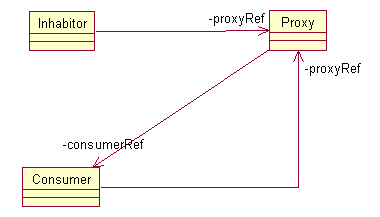
\includegraphics[width=0.5\textwidth]{figures/freshdata.png}
\end{center}
\caption{Class Diagram for Fresh Data Pattern\label{fig:freshdata}}
\end{figure}

The \texttt{Proxy} can then inform the \texttt{Consumer} that data is
available, which the \texttt{Consumer} can access at its own leisure.

The \texttt{Data} class is used to represent the data values used in
the pattern. Thus it is just a place holder and therefore has no
contents in this case.

\begin{lstlisting}
class Data
end Data
\end{lstlisting}

\subsection{The Inhabitor}

The \texttt{Inhabitor} class is used to inhabit the model with data
for testing purposes. It places this data in a \texttt{Proxy}, which
it has a reference to. This reference is stored as an instance
variable.

\begin{lstlisting}
class Inhabitor

instance variables
  proxyRef : Proxy
\end{lstlisting}

The constructor is used to initialize the reference to the
\texttt{Proxy}.

\begin{lstlisting}
operations
  public Inhabitor : Proxy ==> Inhabitor
  Inhabitor (proxy) ==
    proxyRef := proxy;
\end{lstlisting}

\begin{figure}
\begin{center}
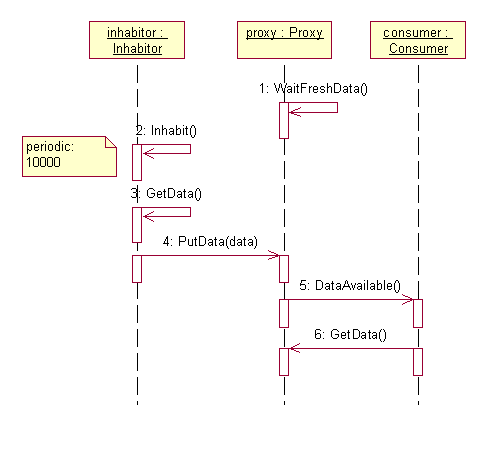
\includegraphics[width=.6\textwidth]{figures/freshdataseqdiag.png}
\end{center}
\caption{Sequence Diagram for Fresh Data Pattern\label{fig:seqdiafresh} }
\end{figure}

Data is sent to the proxy using the \texttt{Inhabit} operation.

\begin{lstlisting}
Inhabit : () ==> ()
Inhabit() ==
  proxyRef.PutData(GetData());
\end{lstlisting}

The operation \texttt{GetData} is used to actually acquire data
values. Here it is left unspecified; in a model it might read data
from a file.

\begin{lstlisting}
GetData : () ==> Data
GetData() ==
  is not yet specified
\end{lstlisting}

The \texttt{Inhabitor} thread calls the \texttt{Inhabit} operation with some
fixed period, here arbitrarily chosen to be 10000 with a jitter allowed to 100
time units and the minimum delay being 9900 time units.

\begin{lstlisting}
thread
  periodic (10000,100,9900,0)(Inhabit)

end Inhabitor
\end{lstlisting}

\subsection{The Proxy}

The \texttt{Proxy} class provides the same interface as that intended
for the actual device it is modelling, but it takes the data that the
device would generate from the \texttt{Inhabitor}.

It has three instance variables:

\begin{description}
\item[\texttt{d}] the data value most recently generated, or {\bf{\ttfamily{nil}}} if no
fresh data exists.
\item[\texttt{freshData}] a Boolean value indicating whether fresh data exists.
\item[\texttt{consumerRef}] a reference to the \texttt{Consumer}.
\end{description}

\begin{lstlisting}
class Proxy

instance variables
  d : [Data] := nil;
  freshData : bool := false;
  consumerRef : Consumer
\end{lstlisting}

The constructor is used to initialize the \texttt{Consumer} reference.

\begin{lstlisting}
operations

public Proxy : Consumer ==> Proxy
Proxy(consumer) ==
  consumerRef := consumer;
\end{lstlisting}

\texttt{PutData} is used by the \texttt{Inhabitor} to send data to the
\texttt{Proxy}.

\begin{lstlisting}
public PutData : Data ==> ()
PutData(newData) ==
  ( d := newData;
    freshData := true
  );
\end{lstlisting}

\texttt{GetData} is used by the \texttt{Consumer} to retrieve fresh
data from the \texttt{Proxy}.

\begin{lstlisting}
public GetData : () ==> Data
GetData() ==
  let od = d in
  ( d := nil;
    return od
  );
\end{lstlisting}

\texttt{WaitFreshData} is used by this class's thread to wait until
fresh data is available.

\begin{lstlisting}
WaitFreshData : () ==> ()
WaitFreshData() ==
  freshData := false;

sync
  per WaitFreshData => freshData
\end{lstlisting}

The thread for this class repeatedly waits for fresh data and then
informs the consumer of its arrival.

\begin{lstlisting}
thread

while true do
( WaitFreshData();
  consumerRef.DataAvailable()
)

end Proxy
\end{lstlisting}

\subsection{The Consumer}

The consumer represents the interface to the remainder of the
system. It takes data values from the \texttt{Proxy} and uses them as
it sees fit.

Three instance variables are defined:

\begin{description}
\item[\texttt{dataAvailable}] a Boolean value indicating whether fresh
data is available or not.
\item[\texttt{proxyRef}] a reference to the \texttt{Proxy}, used to
retrieve data.
\item[\texttt{d}] the data value retrieved from the \texttt{Proxy}.
\end{description}

\begin{lstlisting}
class Consumer

instance variables
  dataAvailable : bool := false;
  proxyRef : Proxy;
  d : Data
\end{lstlisting}

The constructor is used to initialize the reference to the
\texttt{Proxy}.

\begin{lstlisting}
operations
  public Consumer : Proxy ==> Consumer
  Consumer(proxy) ==
    proxyRef := proxy;
\end{lstlisting}

\texttt{DataAvailable} is used by the \texttt{Proxy} to indicate
arrival of fresh data.

\begin{lstlisting}
  public DataAvailable : () ==> ()
  DataAvailable() ==
    dataAvailable := true;
\end{lstlisting}

\texttt{GetData} is used to acquire fresh data from the proxy. It
blocks whenever fresh data is not available.

\begin{lstlisting}
  GetData : () ==> ()
  GetData() ==
    (d := proxyRef.GetData();
     dataAvailable := false
    );

sync
  per GetData => dataAvailable
\end{lstlisting}

The thread for this class repeatedly takes data when it is available.

\begin{lstlisting}
thread

  while true do
    GetData()

end Consumer
\end{lstlisting}

\section{The Time Stamp Pattern}\label{sec:TimeStamp}

The Time Stamp pattern is for use in synchronous systems, where each
different thread has its own execution period. Such threads we refer
to as clients. 
A single instance of a
\texttt{TimeStamp} class will be shared amongst all of the different
clients, and is used to ensure each client is awoken for its execution
period (following the standard singleton design pattern). An example arrangement is shown in
Figure~\ref{fig:classtimestamp} with two client classes included for
illustrative purposes.

Each client executes its
\texttt{ComputationPhase} -- that computation it is intended to perform
periodically. When it completes its \texttt{ComputationPhase} it calls 
\texttt{TimeStamp`WaitRelative} with its
execution period, and is then awoken at that time, or as soon as
possible thereafter. Note that since the clients are incidental to the 
pattern, they are not given in the following specification.

%\texttt{TimeStamp`NotifyAll} 
%is then called in order to release any waiting clients. Finally, the thread 
%blocks on \texttt{TimeStamp`Awake}, where the thread waits until it 
%is time to wake up. 

\subsection{The TimeStamp Class}

The \texttt{TimeStamp} class maintains a map from thread ids to 
time (\texttt{wakeUpMap}), representing when a particular thread 
should be woken. The other instance variable in the class
represents the current time. Note that this concept is orthogonal to
the notion of simulated time described earlier in this document.

%% \begin{figure}
%% \begin{center}
%% 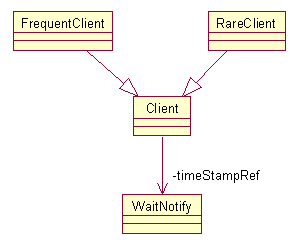
\includegraphics[width=0.5\textwidth]{figures/timestamp.png}
%% \end{center}
%% \caption{Class Diagram for Time Stamp Pattern\label{fig:classtimestamp}}
%% \end{figure}

%\begin{figure}
%\begin{center}
%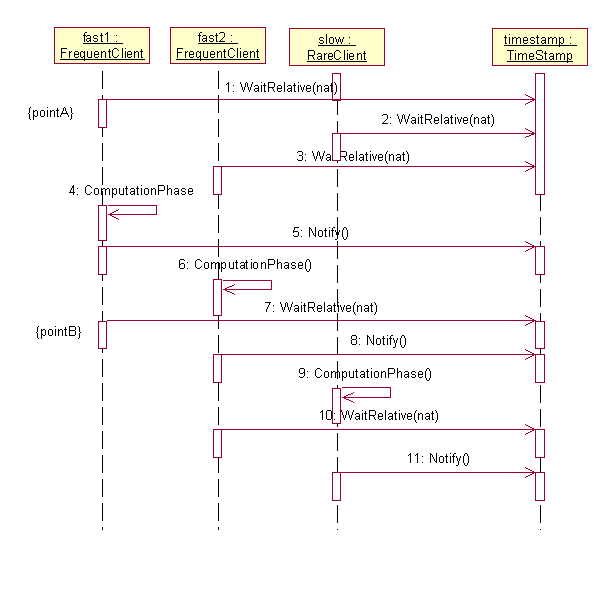
\includegraphics[width=\textwidth]{figures/timestampseqdiag.png}
%\end{center}
%\caption{Sequence Diagram for Time Stamp Pattern\label{fig:seqdiagtimestamp}}
%\end{figure}

\begin{lstlisting}
class TimeStamp

values

public stepLength : nat = 1;

instance variables

currentTime  : nat   := 0;
wakeUpMap    : map nat to [nat] := {|->};
barrierCount : nat := 0;
registeredThreads : set of BaseThread := {};
isInitialising : bool := true;
-- singleton instance of class
private static timeStamp : TimeStamp := new TimeStamp();
\end{lstlisting}

Other classes can access the \texttt{TimeStamp} singleton class using the \texttt{GetInstance} operation.

\begin{lstlisting}
operations

-- private constructor (singleton pattern)
private TimeStamp : () ==> TimeStamp
TimeStamp() ==
  skip;

-- public operation to get the singleton instance
public static GetInstance: () ==> TimeStamp
GetInstance() ==
  return timeStamp;
\end{lstlisting}

Whenever a thread is started it gets registered with a reference to it:

\begin{lstlisting}
public RegisterThread : BaseThread ==> ()
RegisterThread(t) ==
 (barrierCount := barrierCount + 1;
  registeredThreads := registeredThreads union {t};  
 );
 
public UnRegisterThread : BaseThread ==> ()
UnRegisterThread(t) ==
 (barrierCount := barrierCount - 1;
  registeredThreads := registeredThreads \ {t};
 );
\end{lstlisting}

When all threads have registered themselves and initialisation is finished
all these threads can be started.

\begin{lstlisting}
public IsInitialising: () ==> bool
IsInitialising() ==
  return isInitialising;
 
public DoneInitialising: () ==> ()
DoneInitialising() ==
 (if isInitialising
  then (isInitialising := false;
        for all t in set registeredThreads 
        do
          start(t);
       );
 );
\end{lstlisting}

A client may request an absolute wait. using \texttt{WaitRelative}.

\begin{lstlisting}
public WaitRelative : nat ==> ()
WaitRelative(val) ==
  WaitAbsolute(currentTime + val);
\end{lstlisting}

Absolute waits are performed using \texttt{WaitAbsolute}. Note that if time
given is less than the current time, then the client will never be
woken.

\begin{lstlisting}
public WaitAbsolute : nat ==> ()
WaitAbsolute(val) ==
 (AddToWakeUpMap(threadid, val);
  -- Last to enter the barrier notifies the rest.
  BarrierReached();
  -- Wait till time is up
  Awake();
);
\end{lstlisting}

\texttt{AddToWakeUpMap} is used to add new waits to the \texttt{wakeUpMap}.

\begin{lstlisting}
AddToWakeUpMap : nat * nat ==> ()
AddToWakeUpMap(tId, val) ==
  wakeUpMap := wakeUpMap ++ { tId |-> val };
\end{lstlisting}

The operation \texttt{BarrierReached} evaluates the \texttt{wakeUpMap} when 
all period threads have entered the mapping. Time is incremented and all threads
that needs to be awoken is removed from the \texttt{wakeUpMap}.

\begin{lstlisting}
BarrierReached : () ==> ()
BarrierReached() == 
  while  (card dom wakeUpMap = barrierCount) do
   (currentTime := currentTime + stepLength;
    let threadSet : set of nat = {th | th in set dom wakeUpMap 
                                     & wakeUpMap(th) <> nil and 
                                       wakeUpMap(th) <= currentTime }
    in
      for all t in set threadSet 
      do
         wakeUpMap := {t} <-: wakeUpMap;
   )
post forall x in set rng wakeUpMap & x = nil or x >= currentTime;
\end{lstlisting}

All threads block on the operation \texttt{Awake} until they are removed from
the \texttt{wakeUpMap} as described above.

\begin{lstlisting}
operations

Awake: () ==> ()
Awake() == skip;

sync
  per Awake => threadid not in set dom wakeUpMap;
\end{lstlisting}

%A specific thread can be immediately awoken
%using \texttt{NotifyThread}.
%
%\begin{lstlisting}
%public NotifyThread : nat ==> ()
%NotifyThread(tId) ==
%  wakeUpMap := {tId} <-: wakeUpMap;
%\end{lstlisting}

%An arbitrary thread is immediately awoken using \texttt{Notify}.
%
%\begin{lstlisting}
%public Notify : () ==> ()
%Notify() ==
%  let tId in set dom wakeUpMap in
%    NotifyThread(tId);
%\end{lstlisting}

%Testing all waiting threads to find which needs to be awoken using \texttt{NotifyAll}.
%
%\begin{lstlisting}
%public NotifyAll : () ==> ()
%NotifyAll() ==
%  let threadSet : set of nat = {th | th in set dom wakeUpMap 
%                                   & wakeUpMap(th) <= currentTime }
%  in
%    for all t in set threadSet 
%    do
%      NotifyThread(t);
%\end{lstlisting}
%
%The operation \texttt{NotifyAndIncTime} is used to increment time and
%awake all threads waiting for the current time step.
%
%\begin{lstlisting}
%NotifyAndIncTime : () ==> ()
%NotifyAndIncTime() ==
%( currentTime := currentTime + 1;
%  NotifyAll();
%);
%\end{lstlisting}

The current time of the class may be obtained via the \texttt{GetTime}
operation.

\begin{lstlisting}
public GetTime : () ==> nat
GetTime() ==
  return currentTime;
\end{lstlisting}

Since \texttt{barrierCount}, \texttt{registeredThreads} and 
\texttt{wakeUpMap} is manipulated by a number of different
operations, we need to set access to them to be mutually exclusive.

\begin{lstlisting}
sync
  per Awake => threadid not in set dom wakeUpMap;
  mutex (IsInitialising);
  mutex (DoneInitialising); 
  mutex (AddToWakeUpMap);
  mutex (NotifyThread);
  mutex (BarrierReached);  
  mutex (AddToWakeUpMap, NotifyThread);
  mutex (AddToWakeUpMap, BarrierReached);
  mutex (NotifyThread, BarrierReached);  
  mutex (AddToWakeUpMap, NotifyThread, BarrierReached);

end TimeStamp
\end{lstlisting}
 
\chapter{Examples In Full}\label{app:listing}

\section{VDM-SL Model for Counter Measures System}\label{app:VDMSLmodel}

\begin{lstlisting}
types

MissileInputs = seq of MissileInput;

MissileInput = MissileType * Angle;

MissileType = <MissileA> | <MissileB> | <MissileC> | <None>;

Angle = nat
inv num == num <= 360;

Output = map MagId to seq of OutputStep;

MagId = token;

OutputStep = FlareType * AbsTime;

Response = FlareType * nat;

AbsTime = nat;

FlareType = <FlareOneA>  | <FlareTwoA>  | <FlareOneB> |
            <FlareTwoB>  | <FlareOneC>  | <FlareTwoC> |
            <DoNothingA> | <DoNothingB> | <DoNothingC>;

Plan = seq of (FlareType * Delay);

Delay = nat;

values

responseDB : map MissileType to Plan =
{<MissileA> |-> [mk_(<FlareOneA>,900), mk_(<FlareTwoA>,500),
                 mk_(<DoNothingA>,100), mk_(<FlareOneA>,500)],
 <MissileB> |-> [mk_(<FlareTwoB>,500), mk_(<FlareTwoB>,700)],
 <MissileC> |-> [mk_(<FlareOneC>,400), mk_(<DoNothingC>,100),
                 mk_(<FlareTwoC>,400), mk_(<FlareOneC>,500)]
};

missilePriority : map MissileType to nat
                = {<MissileA> |-> 1,
                   <MissileB> |-> 2,
                   <MissileC> |-> 3,
                   <None>     |-> 0};

stepLength : nat = 100;

testval1 : MissileInputs = [mk_(<MissileA>,88),
                            mk_(<MissileB>,70),
                            mk_(<MissileA>,222),
                            mk_(<MissileC>,44)];

testval2 : MissileInputs = [mk_(<MissileC>,188),
                            mk_(<MissileB>,70),
                            mk_(<MissileA>,2),
                            mk_(<MissileC>,44)];

testval3 : MissileInputs = [mk_(<MissileA>,288),
                            mk_(<MissileB>,170),
                            mk_(<MissileA>,222),
                            mk_(<MissileC>,44)];

functions

CounterMeasures: MissileInputs -> Output
CounterMeasures(missileInputs) ==
  CM(missileInputs,{|->},{|->},0);

CM: MissileInputs * Output * map MagId to [MissileType] * 
    nat -> Output
CM( missileInputs, outputSoFar, lastMissile, curTime) ==
  if missileInputs = []
  then outputSoFar
  else let mk_(curMis,angle) = hd missileInputs,
           magid = Angle2MagId(angle)
       in
         if magid not in set dom lastMissile or
            (magid in set dom lastMissile and
             missilePriority(curMis) > 
             missilePriority(lastMissile(magid)))
         then let newOutput = 
                     InterruptPlan(curTime,outputSoFar,
                                   responseDB(curMis),
                                   magid)
              in CM(tl missileInputs, newOutput, 
                    lastMissile ++ {magid |-> curMis},
                    curTime + stepLength)
         else CM(tl missileInputs, outputSoFar, 
                 lastMissile,curTime + stepLength)
measure CMLen;

CMLen: MissileInputs * Output * map MagId to [MissileType] * nat -> nat
CMLen(list,-,-,-) == len list;

InterruptPlan: nat * Output * Plan * MagId -> Output
InterruptPlan(curTime,expOutput,plan,magid) ==
  {magid |-> (if magid in set dom expOutput
              then LeavePrefixUnchanged(expOutput(magid), 
                                        curTime)
              else []) ^
              MakeOutputFromPlan(curTime, plan)} 
  munion
  ({magid} <-: expOutput);

LeavePrefixUnchanged: seq of OutputStep * nat -> 
                      seq of OutputStep
LeavePrefixUnchanged(output_l, curTime) ==
  [output_l(i) | i in set inds output_l
               & let mk_(-,t) = output_l(i) in t <= curTime];

MakeOutputFromPlan : nat * seq of Response -> seq of OutputStep
MakeOutputFromPlan(curTime, response) ==
  let output = OutputAtTimeZero(response) in
    [let mk_(flare,t) = output(i)
     in
       mk_(flare,t+curTime)
    | i in set inds output];

OutputAtTimeZero : seq of Response -> seq of OutputStep
OutputAtTimeZero(response) ==
  let absTimes = RelativeToAbsoluteTimes(response) in
    let mk_(firstFlare,-) = hd absTimes in
      [mk_(firstFlare,0)] ^
      [ let mk_(-,t) = absTimes(i-1),
            mk_(f,-) = absTimes(i) in
          mk_(f,t) | i in set {2,...,len absTimes}];

RelativeToAbsoluteTimes : seq of Response -> 
                          seq of (FlareType * nat)
RelativeToAbsoluteTimes(ts) ==
  if ts = []
  then []
  else let mk_(f,t) = hd ts,
           ns = RelativeToAbsoluteTimes(tl ts) in
         [mk_(f,t)] ^ [ let mk_(nf, nt) = ns(i)
                        in mk_(nf, nt + t)
                      | i in set inds ns]
measure RespLen;

RespLen: seq of Response -> nat
RespLen(l) ==
  len l;

Angle2MagId: Angle -> MagId
Angle2MagId(angle) ==
  if angle < 90
  then mk_token("Magazine 1")
  elseif angle < 180
  then mk_token("Magazine 2")
  elseif angle < 270
  then mk_token("Magazine 3")
  else mk_token("Magazine 4");
\end{lstlisting}

\section{Sequential VDM++ Model for Counter Measures System}

\subsection{The CM Class}

\begin{lstlisting}
class CM

instance variables

-- maintain a link to the detector
public static detector : MissileDetector := new MissileDetector();

public static sensor0 : Sensor := new Sensor(detector,0);
public static sensor1 : Sensor := new Sensor(detector,90);
public static sensor2 : Sensor := new Sensor(detector,180);
public static sensor3 : Sensor := new Sensor(detector,270);

public static controller0 : FlareController := new FlareController(0);
public static controller1 : FlareController := new FlareController(120);
public static controller2 : FlareController := new FlareController(240);

public static dispenser0 : FlareDispenser := new FlareDispenser(0);
public static dispenser1 : FlareDispenser := new FlareDispenser(30);
public static dispenser2 : FlareDispenser := new FlareDispenser(60);
public static dispenser3 : FlareDispenser := new FlareDispenser(90);

public static dispenser4 : FlareDispenser := new FlareDispenser(0);
public static dispenser5 : FlareDispenser := new FlareDispenser(30);
public static dispenser6 : FlareDispenser := new FlareDispenser(60);
public static dispenser7 : FlareDispenser := new FlareDispenser(90);

public static dispenser8 : FlareDispenser := new FlareDispenser(0);
public static dispenser9 : FlareDispenser := new FlareDispenser(30);
public static dispenser10 : FlareDispenser := new FlareDispenser(60);
public static dispenser11 : FlareDispenser := new FlareDispenser(90);

end CM
\end{lstlisting}

\subsection{The World Class}

\begin{lstlisting}
class World

instance variables
  
-- maintain a link to the environment
public static env : [Environment] := nil;
public static timerRef : Timer := Timer`GetInstance();

operations

public World: () ==> World
World () ==
  (-- set-up the sensors
   env := new Environment("scenario.txt");
   env.addSensor(CM`sensor0);
   env.addSensor(CM`sensor1);
   env.addSensor(CM`sensor2);
   env.addSensor(CM`sensor3);

   -- add the first controller with four dispensers
   CM`controller0.addDispenser(CM`dispenser0);
   CM`controller0.addDispenser(CM`dispenser1);
   CM`controller0.addDispenser(CM`dispenser2);
   CM`controller0.addDispenser(CM`dispenser3);
   CM`detector.addController(CM`controller0);

   -- add the second controller with four dispensers
   CM`controller1.addDispenser(CM`dispenser4);
   CM`controller1.addDispenser(CM`dispenser5);
   CM`controller1.addDispenser(CM`dispenser6);
   CM`controller1.addDispenser(CM`dispenser7);
   CM`detector.addController(CM`controller1);
 
   -- add the third controller with four dispensers
   CM`controller2.addDispenser(CM`dispenser8);
   CM`controller2.addDispenser(CM`dispenser9);
   CM`controller2.addDispenser(CM`dispenser10);
   CM`controller2.addDispenser(CM`dispenser11);
   CM`detector.addController(CM`controller2);
  );

-- the run function blocks the user-interface thread
-- until all missiles in the file have been processed
public Run: () ==> ()
Run () == 
  env.Run()

end World
\end{lstlisting}

\subsection{The Global Class}

\begin{lstlisting}
class GLOBAL

values

public SENSOR_APERTURE = 90;
public FLARE_APERTURE = 120;
public DISPENSER_APERTURE = 30

types

-- there are three different types of missiles
public 
MissileType = <MissileA> | <MissileB> | <MissileC> | <None>;

-- there are nine different flare types, three per missile
public FlareType =
    <FlareOneA> | <FlareTwoA> | <DoNothingA> | 
    <FlareOneB> | <FlareTwoB> | <DoNothingB> | 
    <FlareOneC> | <FlareTwoC> | <DoNothingC>;

-- the angle at which the missile is incoming
public Angle = nat
inv num == num <= 360;

public EventId = nat;

public Time = nat

operations

public canObserve: Angle * Angle * Angle ==> bool
canObserve (pangle, pleft, psize) ==
  def pright = (pleft + psize) mod 360 in
    if pright < pleft
    -- check between [0,pright> and [pleft,360>
    then return (pangle < pright or pangle >= pleft)
    -- check between [pleft, pright>
    else return (pangle >= pleft and pangle < pright);
       
public getAperture: () ==> Angle * Angle
getAperture () == is subclass responsibility;

end GLOBAL
\end{lstlisting}

\subsection{The Environment Class}

\begin{lstlisting}
class Environment is subclass of GLOBAL

types

public inline  = EventId * MissileType * Angle * Time;
public outline = EventId * FlareType * Angle * Time * Time;

instance variables

-- access to the VDMTools stdio
io : IO := new IO();

-- the input file to process
inlines : seq of inline := [];

-- the output file to print
outlines : seq of outline := [];

-- maintain a link to all sensors
ranges : map nat to (Angle * Angle) := {|->};
sensors : map nat to Sensor := {|->};
inv dom ranges = dom sensors;

-- information about the latest event that has arrived
evid : [EventId] := nil;

busy : bool := true;

operations

public Environment: seq of char ==> Environment
Environment (fname) ==
  def mk_ (-,input) = io.freadval[seq of inline](fname) in
    inlines := input;

public addSensor: Sensor ==> ()
addSensor (psens) ==
  (dcl id : nat := card dom ranges + 1;
   atomic (
    ranges := ranges munion {id |-> psens.getAperture()};
    sensors := sensors munion {id |-> psens} 
   )
  );

public Run: () ==> ()
Run () == 
 (while not (isFinished() and CM`detector.isFinished()) do
    (evid := createSignal();
     CM`detector.Step();
     World`timerRef.StepTime();
    );
 showResult()
 );

private createSignal: () ==> [EventId]
createSignal () ==
  (if len inlines > 0
   then (dcl curtime : Time := World`timerRef.GetTime(), 
             done : bool := false;
         while not done do
           def mk_ (eventid, pmt, pa, pt) = hd inlines in
             if pt <= curtime
             then (for all id in set dom ranges do
                     def mk_(papplhs,pappsize) = ranges(id) in
                       if canObserve(pa,papplhs,pappsize)
                       then sensors(id).trip(eventid,pmt,pa);
                   inlines := tl inlines;
                   done := len inlines = 0;
                   return eventid )
             else (done := true;
                   return nil ))
   else (busy := false;
         return nil));

public handleEvent: EventId * FlareType * Angle * Time * Time ==> ()
handleEvent (newevid,pfltp,angle,pt1,pt2) ==
  (outlines := outlines ^ [mk_ (newevid,pfltp, angle,pt1, pt2)] );

public showResult: () ==> ()
showResult () ==
  def - = io.writeval[seq of outline](outlines) in skip;

public isFinished : () ==> bool
isFinished () == 
  return inlines = [] and not busy;

end Environment
\end{lstlisting}

\subsection{The Sensor Class}

\begin{lstlisting}
class Sensor is subclass of GLOBAL

instance variables

-- the missile detector this sensor is connected to
private detector : MissileDetector;

-- the left hand-side of the viewing angle of the sensor
private aperture : Angle;

operations

public Sensor: MissileDetector * Angle ==> Sensor
Sensor (pmd, psa) == ( detector := pmd; aperture := psa);

-- get the left hand-side start point and opening angle
public getAperture: () ==> GLOBAL`Angle * GLOBAL`Angle
getAperture () == return mk_ (aperture, SENSOR_APERTURE);

-- trip is called asynchronously from the environment to
-- signal an event. the sensor triggers if the event is
-- in the field of view. the event is stored in the
-- missile detector for further processing
public trip: EventId * MissileType * Angle ==> ()
trip (evid, pmt, pa) ==
  -- log and time stamp the observed threat
  detector.addThreat(evid, pmt,pa,World`timerRef.GetTime())
pre canObserve(pa, aperture, SENSOR_APERTURE)

end Sensor
\end{lstlisting}

\subsection{The Missile Detector Class}

\begin{lstlisting}
class MissileDetector is subclass of GLOBAL

-- the primary task of the MissileDetector is to
-- collect all sensor data and dispatch each event
-- to the appropriate FlareController

instance variables

-- maintain a link to each controller
ranges : map nat to (Angle * Angle) := {|->};
controllers : map nat to FlareController := {|->};
inv dom ranges = dom controllers;

-- collects the observations from all attached sensors
threats : seq of (EventId * MissileType * Angle * Time) := [];

-- status of the missile detector
busy : bool := false

operations

-- addController is only used to instantiate the model
public addController: FlareController ==> ()
addController (pctrl) ==
  (dcl nid : nat := card dom ranges + 1;
   atomic
    (ranges := ranges munion {nid |-> pctrl.getAperture()};
     controllers := controllers munion {nid |-> pctrl}
    );
  );

public Step: () ==> ()
Step() ==
  (if threats <> []
   then def mk_ (evid,pmt, pa, pt) = getThreat() in
          for all id in set dom ranges do
            def mk_(papplhs, pappsize) = ranges(id) in
              if canObserve(pa, papplhs, pappsize)
              then controllers(id).addThreat(evid,pmt,pa,pt);
    busy := len threats > 0;
    for all id in set dom controllers do
      controllers(id).Step()
  );
 
-- addThreat is a helper operation to modify the event
-- list. currently events are stored first come first served.
-- one could imagine using a different ordering instead.
public addThreat: EventId * MissileType * Angle * Time ==> ()
addThreat (evid,pmt,pa,pt) == 
  (threats := threats ^ [mk_ (evid,pmt,pa,pt)];
   busy := true );

-- getThreat is a local helper operation to modify the event list
private getThreat: () ==> EventId * MissileType * Angle * Time
getThreat () ==
  (dcl res : EventId * MissileType * Angle * Time := hd threats;
   threats := tl threats;
   return res );

public isFinished: () ==> bool
isFinished () ==
  return forall id in set dom controllers &
            controllers(id).isFinished()

end MissileDetector
\end{lstlisting}

\subsection{The Flare Controller Class}

\begin{lstlisting}
class FlareController is subclass of GLOBAL

instance variables

-- the left hand-side of the working angle
private aperture : Angle;

-- maintain a link to each dispenser
ranges : map nat to (Angle * Angle) := {|->};
dispensers : map nat to FlareDispenser := {|->};
inv dom ranges = dom dispensers;

-- the relevant events to be treated by this controller
threats : seq of (EventId * MissileType * Angle * Time) := [];

-- the status of the controller
busy : bool := false

operations

public FlareController: Angle ==> FlareController
FlareController (papp) == aperture := papp;

public addDispenser: FlareDispenser ==> ()
addDispenser (pfldisp) ==
  let angle = aperture + pfldisp.GetAngle() in
    (dcl id : nat := card dom ranges + 1;
     atomic
     (ranges := ranges munion 
                {id |-> mk_(angle, DISPENSER_APERTURE)};
      dispensers := dispensers munion {id |-> pfldisp});
     );

public Step: () ==> ()
Step() ==
  (if threats <> []
   then def mk_ (evid,pmt, pa, pt) = getThreat() in
          for all id in set dom ranges do
            def mk_(papplhs, pappsize) = ranges(id) in
              if canObserve(pa, papplhs, pappsize)
              then dispensers(id).addThreat(evid,pmt,pt);
   busy := len threats > 0;
   for all id in set dom dispensers do
     dispensers(id).Step());
 
-- get the left hand-side start point and opening angle
public getAperture: () ==> GLOBAL`Angle * GLOBAL`Angle
getAperture () == return mk_(aperture, FLARE_APERTURE);

-- addThreat is a helper operation to modify the event
-- list. currently events are stored first come first served.
-- one could imagine using a different ordering instead
public addThreat: EventId * MissileType * Angle * Time ==> ()
addThreat (evid,pmt,pa,pt) ==
  (threats := threats ^ [mk_ (evid,pmt,pa,pt)];
   busy := true );

-- getThreat is a local helper operation to modify the event list
private getThreat: () ==> EventId * MissileType * Angle * Time
getThreat () ==
  (dcl res : EventId * MissileType * Angle * Time := hd threats;
   threats := tl threats;
   return res );

public isFinished: () ==> bool
isFinished () ==
  return forall id in set dom dispensers &
            dispensers(id).isFinished();

end FlareController
\end{lstlisting}

\subsection{The Flare Dispenser Class}

\begin{lstlisting}
class FlareDispenser is subclass of GLOBAL

values

responseDB : map MissileType to Plan =
  {<MissileA> |-> [mk_(<FlareOneA>,900),
                   mk_(<FlareTwoA>,500),
                   mk_(<DoNothingA>,100),
                   mk_(<FlareOneA>,500)],
   <MissileB> |-> [mk_(<FlareTwoB>,500),
                   mk_(<FlareTwoB>,700)],
   <MissileC> |-> [mk_(<FlareOneC>,400),
                   mk_(<DoNothingC>,100),
                   mk_(<FlareTwoC>,400),
                   mk_(<FlareOneC>,500)] };

missilePriority : map MissileType to nat =
  {<None>     |-> 0,
   <MissileA> |-> 1,
   <MissileB> |-> 2,
   <MissileC> |-> 3 }

types

public Plan = seq of PlanStep;

public PlanStep = FlareType * Time;

instance variables

public curplan : Plan := [];
curprio        : nat := 0;
busy           : bool := false;
aperture       : Angle;
eventid        : [EventId];

operations

public FlareDispenser: nat ==> FlareDispenser
FlareDispenser(ang) ==
  aperture := ang;
  
public Step: () ==> ()
Step() ==
  if len curplan > 0
  then (dcl curtime : Time := World`timerRef.GetTime(),
            first : PlanStep := hd curplan,
            next : Plan := tl curplan;
        let mk_(fltp, fltime) = first in
          (if fltime <= curtime
           then (releaseFlare(eventid,fltp,fltime,curtime);
                 curplan := next;
                 if len next = 0
                 then (curprio := 0; 
                       busy := false ) )
           )
    );

public GetAngle: () ==> nat
GetAngle() ==
  return aperture;

public addThreat: EventId * MissileType * Time ==> ()
addThreat (evid, pmt, ptime) ==
  if missilePriority(pmt) > curprio
  then (dcl newplan : Plan :=  [],
            newtime : Time := ptime;
        -- construct an absolute time plan
        for mk_(fltp, fltime) in responseDB(pmt) do
          (newplan := newplan ^ [mk_ (fltp, newtime)];
           newtime := newtime + fltime );
        -- immediately release the first action
        def mk_(fltp, fltime) = hd newplan;
            t = World`timerRef.GetTime() in
          releaseFlare(evid,fltp,fltime,t);
        -- store the rest of the plan
        curplan := tl newplan;
        eventid := evid;
        curprio := missilePriority(pmt);
        busy := true )
pre pmt in set dom missilePriority and
    pmt in set dom responseDB;

private releaseFlare: EventId * FlareType * Time * Time ==> ()
releaseFlare (evid,pfltp, pt1, pt2) == 
  World`env.handleEvent(evid,pfltp,aperture,pt1,pt2);

public isFinished: () ==> bool
isFinished () == 
  return not busy

end FlareDispenser
\end{lstlisting}

\subsection{The Timer Class}\label{sec:timerapp}

\begin{lstlisting}
class Timer

instance variables

currentTime : nat := 0;
private static timerInstance : Timer := new Timer(); 

values

stepLength : nat = 10;

operations

private Timer: () ==> Timer
Timer() ==
  skip;
  
public static GetInstance: () ==> Timer
GetInstance() ==
  return timerInstance;

public StepTime : () ==> ()
StepTime() ==
  currentTime := currentTime + stepLength;

public GetTime : () ==> nat
GetTime() ==
  return currentTime;

end Timer
\end{lstlisting}

\subsection{The IO Class}

\begin{lstlisting}
class IO

-- 	Overture STANDARD LIBRARY: INPUT/OUTPUT
--      --------------------------------------------
-- 
-- Standard library for the Overture Interpreter. When the interpreter
-- evaluates the preliminary functions/operations in this file,
-- corresponding internal functions is called instead of issuing a run
-- time error. Signatures should not be changed, as well as name of
-- module (VDM-SL) or class (VDM++). Pre/post conditions is 
-- fully user customisable. 
-- Dont care's may NOT be used in the parameter lists.
--
-- The in/out functions  will return false if an error occurs. In this
-- case an internal error string will be set (see 'ferror').

types
 
public
filedirective = <start>|<append> 

functions

-- Write VDM value in ASCII format to std out:
public
writeval[@p]: @p -> bool
writeval(val)==
  is not yet specified;

-- Write VDM value in ASCII format to file.
-- fdir = <start> will overwrite existing file,
-- fdir = <append> will append output to the file (created if
-- not existing).
public
fwriteval[@p]:seq1 of char * @p * filedirective -> bool
fwriteval(filename,val,fdir) ==
  is not yet specified;

-- Read VDM value in ASCII format from file
public
freadval[@p]:seq1 of char -> bool * [@p]
freadval(f) ==
  is not yet specified
  post let mk_(b,t) = RESULT in not b => t = nil;

operations

-- Write text to std out. Surrounding double quotes will be stripped,
-- backslashed characters should be interpreted.
public
echo: seq of char ==> bool
echo(text) ==
  fecho ("",text,nil);

-- Write text to file like 'echo'
public
fecho: seq of char * seq of char * [filedirective] ==> bool
fecho (filename,text,fdir) ==
  is not yet specified
  pre filename = "" <=> fdir = nil;

-- The in/out functions  will return false if an error occur. In this
-- case an internal error string will be set. 'ferror' returns this
-- string and set it to "".
public
ferror:()  ==> seq of char
ferror () ==
  is not yet specified;
  
-- New simplified format printing operations
-- The questionmark in the signature simply means any type
public static print: ? ==> ()
print(arg) ==
  is not yet specified;

-- New simplified format printing operations
-- The questionmark in the signature simply means any type
public static printf: seq of char * seq of ? ==> ()
printf(format, args) ==
  is not yet specified;

end IO
\end{lstlisting}

\section{Concurrent VDM++ Model for Counter Measures System}\label{app:concurCM}
\subsection{The CM Class}

\begin{lstlisting}
class CM

instance variables
  -- maintain a link to the detector
  public static detector : MissileDetector := new MissileDetector(nil);

  public static sensor0 : Sensor := new Sensor(detector,0);
  public static sensor1 : Sensor := new Sensor(detector,90);
  public static sensor2 : Sensor := new Sensor(detector,180);
  public static sensor3 : Sensor := new Sensor(detector,270);

  public static controller0 : FlareController := new FlareController(0, nil);
  public static controller1 : FlareController := new FlareController(120, nil);
  public static controller2 : FlareController := new FlareController(240, nil);

  public static dispenser0 : FlareDispenser := new FlareDispenser(0, nil);
  public static dispenser1 : FlareDispenser := new FlareDispenser(30, nil);
  public static dispenser2 : FlareDispenser := new FlareDispenser(60, nil);
  public static dispenser3 : FlareDispenser := new FlareDispenser(90, nil);

  public static dispenser4 : FlareDispenser := new FlareDispenser(0, nil);
  public static dispenser5 : FlareDispenser := new FlareDispenser(30, nil);
  public static dispenser6 : FlareDispenser := new FlareDispenser(60, nil);
  public static dispenser7 : FlareDispenser := new FlareDispenser(90, nil);

  public static dispenser8 : FlareDispenser := new FlareDispenser(0, nil);
  public static dispenser9 : FlareDispenser := new FlareDispenser(30, nil);
  public static dispenser10 : FlareDispenser := new FlareDispenser(60, nil);
  public static dispenser11 : FlareDispenser := new FlareDispenser(90, nil);

end CM
\end{lstlisting}

\subsection{The World Class}

\begin{lstlisting}
class World

instance variables

public static timerRef : TimeStamp := TimeStamp`GetInstance();
public static env : [Environment] := nil;

operations

public World: () ==> World
World () ==
  (-- set-up the sensors
   env := new Environment("scenario.txt", nil);
   
   env.addSensor(CM`sensor0);
   env.addSensor(CM`sensor1);
   env.addSensor(CM`sensor2);
   env.addSensor(CM`sensor3);

   -- add the first controller with four dispensers
   CM`controller0.addDispenser(CM`dispenser0);
   CM`controller0.addDispenser(CM`dispenser1);
   CM`controller0.addDispenser(CM`dispenser2);
   CM`controller0.addDispenser(CM`dispenser3);
   CM`detector.addController(CM`controller0);

   -- add the second controller with four dispensers
   CM`controller1.addDispenser(CM`dispenser4);
   CM`controller1.addDispenser(CM`dispenser5);
   CM`controller1.addDispenser(CM`dispenser6);
   CM`controller1.addDispenser(CM`dispenser7);
   CM`detector.addController(CM`controller1);
 
   -- add the third controller with four dispensers
   CM`controller2.addDispenser(CM`dispenser8);
   CM`controller2.addDispenser(CM`dispenser9);
   CM`controller2.addDispenser(CM`dispenser10);
   CM`controller2.addDispenser(CM`dispenser11);
   CM`detector.addController(CM`controller2);   
   );

-- the run function blocks the user-interface thread
-- until all missiles in the file have been processed
public Run: () ==> ()
Run () == 
  (-- start the environment
   timerRef.DoneInitialising();
   -- wait for the environment to handle all input
   env.isFinished();
   -- wait for the missile detector to finish
   CM`detector.isFinished();
   -- print the result
   env.showResult())

end World
\end{lstlisting}

\subsection{The Global Class}

\begin{lstlisting}
class GLOBAL

values

public SENSOR_APERTURE = 90;
public FLARE_APERTURE = 120;
public DISPENSER_APERTURE = 30

types

-- there are three different types of missiles
public MissileType = <MissileA> | <MissileB> | <MissileC> | <None>;

-- there are nine different flare types, three per missile
public FlareType =
    <FlareOneA> | <FlareTwoA> | <DoNothingA> | 
    <FlareOneB> | <FlareTwoB> | <DoNothingB> | 
    <FlareOneC> | <FlareTwoC> | <DoNothingC>;

-- the angle at which the missile is incoming
public Angle = nat
inv num == num < 360;

public EventId = nat;

public Time = nat;

operations

public canObserve: Angle * Angle * Angle ==> bool
canObserve (pangle, pleft, psize) ==
  def pright = (pleft + psize) mod 360 in
    if pright < pleft
    -- check between [0,pright> and [pleft,360>
    then return (pangle < pright or pangle >= pleft)
    -- check between [pleft, pright>
    else return (pangle >= pleft and pangle < pright);

end GLOBAL
\end{lstlisting}

\subsection{The Environment Class}

\begin{lstlisting}
class Environment is subclass of GLOBAL, BaseThread

types

public InputTP   = (Time * seq of inline);

public inline  = EventId * MissileType * Angle * Time;
public outline = EventId * FlareType * Angle * Time * Time

instance variables

-- access to the VDMTools stdio
io : IO := new IO();

-- the input file to process
inlines : seq of inline := [];

-- the output file to print
outlines : seq of outline := [];

-- maintain a link to all sensors
ranges : map nat to (Angle * Angle) := {|->};
sensors : map nat to Sensor := {|->};
inv dom ranges = dom sensors;

busy : bool := true;

-- Amount of time we want to simulate
simtime : Time;

operations

public Environment: seq of char * [ThreadDef] ==> Environment
Environment (fname, tDef) ==
 (def mk_ (-,mk_(timeval,input)) = io.freadval[InputTP](fname) in
    (inlines := input;
     simtime := timeval);
     
  if tDef <> nil
  then (period := tDef.p;
        isPeriodic := tDef.isP;
       );
  BaseThread(self);
  );

public addSensor: Sensor ==> ()
addSensor (psens) ==
  (dcl id : nat := card dom ranges + 1;
   atomic (
    ranges := ranges munion {id |-> psens.getAperture()};
    sensors := sensors munion {id |-> psens} 
   )
  );

private createSignal: () ==> () 
createSignal () ==
  (if len inlines > 0
   then (dcl curtime : Time := World`timerRef.GetTime(), 
             done : bool := false;
         while not done do
           def mk_ (eventid, pmt, pa, pt) = hd inlines in
             if pt <= curtime
             then (for all id in set dom ranges do
                     def mk_(papplhs,pappsize) = ranges(id) in
                       if canObserve(pa,papplhs,pappsize)
                       then sensors(id).trip(eventid,pmt,pa);
                   inlines := tl inlines;
                   done := len inlines = 0;
                   return) 
             else (done := true;
                   return))
   else (busy := false;
         return));

public handleEvent: EventId * FlareType * Angle * Time * Time ==> ()
handleEvent (evid,pfltp,angle,pt1,pt2) ==
  (outlines := outlines ^ [mk_ (evid,pfltp,angle,pt1,pt2)] );

public showResult: () ==> ()
showResult () ==
  def - = io.writeval[seq of outline](outlines) in skip;

public isFinished : () ==> ()
isFinished () == skip;

public Step : () ==> ()
Step() ==
 (if World`timerRef.GetTime() < simtime
  then createSignal()
  else busy := false;
 );
 
sync

mutex (handleEvent);
mutex (createSignal);
per isFinished => not busy;

end Environment
\end{lstlisting}

\subsection{The Sensor Class}

\begin{lstlisting}
class Sensor is subclass of GLOBAL

instance variables

-- the missile detector this sensor is connected to
private detector : MissileDetector;

-- the left hand-side of the viewing angle of the sensor
private aperture : Angle;

operations

public Sensor: MissileDetector * Angle ==> Sensor
Sensor (pmd, psa) == ( detector := pmd; aperture := psa);

-- get the left hand-side start point and opening angle
public getAperture: () ==> GLOBAL`Angle * GLOBAL`Angle
getAperture () == return mk_ (aperture, SENSOR_APERTURE);

-- trip is called asynchronously from the environment to
-- signal an event. the sensor triggers if the event is
-- in the field of view. the event is stored in the
-- missile detector for further processing
public trip: EventId * MissileType * Angle ==> ()
trip (evid, pmt, pa) ==
  -- log and time stamp the observed threat
  detector.addThreat(evid, pmt,pa,World`timerRef.GetTime())
pre canObserve(pa, aperture, SENSOR_APERTURE)

end Sensor
\end{lstlisting}

\subsection{The Missile Detector Class}

\begin{lstlisting}
class MissileDetector is subclass of GLOBAL, BaseThread

-- the primary task of the MissileDetector is to
-- collect all sensor data and dispatch each event
-- to the appropriate FlareController

instance variables

-- maintain a link to each controller
ranges : map nat to (Angle * Angle) := {|->};
controllers : map nat to FlareController := {|->};
inv dom ranges = dom controllers;

-- collects the observations from all attached sensors
threats : seq of (EventId * MissileType * Angle * Time) := [];

-- status of the missile detector
busy : bool := false

operations

public MissileDetector: [ThreadDef] ==> MissileDetector
MissileDetector(tDef)==
 (if tDef <> nil
  then (period := tDef.p;
        isPeriodic := tDef.isP;
       );
  BaseThread(self);
 );

-- addController is only used to instantiate the model
public addController: FlareController ==> ()
addController (pctrl) ==
  (dcl nid : nat := card dom ranges + 1;
   atomic
    (ranges := ranges munion {nid |-> pctrl.getAperture()};
     controllers := controllers munion {nid |-> pctrl}
    );
   );

-- addThreat is a helper operation to modify the event
-- list. currently events are stored first come first served.
-- one could imagine using a different ordering instead.
public addThreat: EventId * MissileType * Angle * Time ==> ()
addThreat (evid,pmt,pa,pt) == 
  (threats := threats ^ [mk_ (evid,pmt,pa,pt)];
   busy := true );

-- getThreat is a local helper operation to modify the event list
private getThreat: () ==> EventId * MissileType * Angle * Time
getThreat () ==
  (dcl res : EventId * MissileType * Angle * Time := hd threats;
   threats := tl threats;
   return res );

public isFinished: () ==> ()
isFinished () ==
  for all id in set dom controllers do
    controllers(id).isFinished();

Step: () ==> ()
Step() ==
( if threats <> []
  then (def mk_ (evid,pmt, pa, pt) = getThreat() in
          for all id in set dom ranges do
            def mk_(papplhs, pappsize) = ranges(id) in
              if canObserve(pa, papplhs, pappsize)
              then controllers(id).addThreat(evid,pmt,pa,pt);
        busy := len threats > 0);
);
 
sync
  mutex (Step);

  -- addThreat and getThreat modify the same instance variables
  -- therefore they need to be declared mutual exclusive
  mutex (addThreat,getThreat);

  -- getThreat is used as a 'blocking read' from the main
  -- thread of control of the missile detector
  per getThreat => len threats > 0;
  per isFinished => not busy

end MissileDetector
\end{lstlisting}

\subsection{The Flare Controller Class}

\begin{lstlisting}
class FlareController is subclass of GLOBAL, BaseThread

instance variables

-- the left hand-side of the working angle
private aperture : Angle;

-- maintain a link to each dispenser
ranges : map nat to (Angle * Angle) := {|->};
dispensers : map nat to FlareDispenser := {|->};
inv dom ranges = dom dispensers;

-- the relevant events to be treated by this controller
threats : seq of (EventId * MissileType * Angle * Time) := [];

-- the status of the controller
busy : bool := false

operations

public FlareController: Angle * [ThreadDef] ==> FlareController
FlareController (papp, tDef) == 
 (aperture := papp;
 
  if tDef <> nil
  then (period := tDef.p;
        isPeriodic := tDef.isP;
       );
  BaseThread(self);
 );

public addDispenser: FlareDispenser ==> ()
addDispenser (pfldisp) ==
  let angle = aperture + pfldisp.GetAngle() in
    (dcl id : nat := card dom ranges + 1;
     atomic
      (ranges := ranges munion 
                 {id |-> mk_(angle, DISPENSER_APERTURE)};
       dispensers := dispensers munion {id |-> pfldisp}
      );
     );

-- get the left hand-side start point and opening angle
public getAperture: () ==> GLOBAL`Angle * GLOBAL`Angle
getAperture () == return mk_(aperture, FLARE_APERTURE);

-- addThreat is a helper operation to modify the event
-- list. currently events are stored first come first served.
-- one could imagine using a different ordering instead
public addThreat: EventId * MissileType * Angle * Time ==> ()
addThreat (evid,pmt,pa,pt) ==
  (threats := threats ^ [mk_ (evid,pmt,pa,pt)];
   busy := true );

-- getThreat is a local helper operation to modify the event list
private getThreat: () ==> EventId * MissileType * Angle * Time
getThreat () ==
  (dcl res : EventId * MissileType * Angle * Time := hd threats;
   threats := tl threats;
   return res );

public isFinished: () ==> ()
isFinished () ==
  for all id in set dom dispensers do
    dispensers(id).isFinished();

Step: () ==> ()
Step() ==
  (if threats <> []
  then (def mk_ (evid,pmt, pa, pt) = getThreat() in
         for all id in set dom ranges do
           def mk_(papplhs, pappsize) = ranges(id) in
             if canObserve(pa, papplhs, pappsize)
             then dispensers(id).addThreat(evid,pmt,pt);
        busy := len threats > 0 );
       );

sync

-- addThreat and getThreat modify the same instance variables
-- therefore they need to be declared mutual exclusive
mutex (addThreat,getThreat);
mutex (Step);

-- getThreat is used as a 'blocking read' from the main
-- thread of control of the missile detector
per getThreat => len threats > 0;
per isFinished => len threats = 0 --not busy

end FlareController
\end{lstlisting}

\subsection{The Flare Dispenser Class}

\begin{lstlisting}
class FlareDispenser is subclass of GLOBAL, BaseThread

values

responseDB : map MissileType to Plan =
  {<MissileA> |-> [mk_(<FlareOneA>,900),
                   mk_(<FlareTwoA>,500),
                   mk_(<DoNothingA>,100),
                   mk_(<FlareOneA>,500)],
   <MissileB> |-> [mk_(<FlareTwoB>,500),
                   mk_(<FlareTwoB>,700)],
   <MissileC> |-> [mk_(<FlareOneC>,400),
                   mk_(<DoNothingC>,100),
                   mk_(<FlareTwoC>,400),
                   mk_(<FlareOneC>,500)] };

missilePriority : map MissileType to nat =
  {<None>     |-> 0,
   <MissileA> |-> 1,
   <MissileB> |-> 2,
   <MissileC> |-> 3 }

types

public Plan = seq of PlanStep;

public PlanStep = FlareType * Time;

instance variables

public curplan : Plan := [];
curprio        : nat := 0;
busy           : bool := false;
aperture       : Angle;
eventid        : [EventId];

operations

public FlareDispenser: Angle * [ThreadDef] ==> FlareDispenser
FlareDispenser(ang, tDef) ==
 (aperture := ang;
 
  if tDef <> nil
  then (period := tDef.p;
        isPeriodic := tDef.isP;
       );
  BaseThread(self);
 );

public GetAngle: () ==> nat
GetAngle() ==
  return aperture;

public addThreat: EventId * MissileType * Time ==> ()
addThreat (evid, pmt, ptime) ==
  if missilePriority(pmt) > curprio
  then (dcl newplan : Plan :=  [],
            newtime : Time := ptime;
        -- construct an absolute time plan
        for mk_(fltp, fltime) in responseDB(pmt) do
          (newplan := newplan ^ [mk_ (fltp, newtime)];
           newtime := newtime + fltime );
        -- immediately release the first action
        def mk_(fltp, fltime) = hd newplan;
            t = World`timerRef.GetTime() in
          releaseFlare(evid,fltp,fltime,t);
         -- store the rest of the plan
         curplan := tl newplan;
         eventid := evid;
         curprio := missilePriority(pmt);
         busy := true )
pre pmt in set dom missilePriority and
    pmt in set dom responseDB;

private Step: () ==> ()
Step () ==
  (if len curplan > 0
   then (dcl curtime : Time := World`timerRef.GetTime(),
             done : bool := false;
         while not done do
           (dcl first : PlanStep := hd curplan,
                next : Plan := tl curplan;
            let mk_(fltp, fltime) = first in
              if fltime <= curtime
              then (releaseFlare(eventid,fltp,fltime,curtime);
                    curplan := next;
                    if len next = 0
                    then (curprio := 0; 
                          done := true; 
                          busy := false ) )
              else done := true ) ) );

private releaseFlare: EventId * FlareType * Time * Time ==> ()
releaseFlare (evid, pfltp, pt1, pt2) == 
  World`env.handleEvent(evid,pfltp,aperture,pt1,pt2);

public isFinished: () ==> ()
isFinished () == skip;

sync

mutex (Step);
mutex (addThreat);
per isFinished => not busy
     
end FlareDispenser
\end{lstlisting}


\subsection{The TimeStamp Class}

\begin{lstlisting}
class TimeStamp

values

public stepLength : nat = 1;

instance variables

currentTime  : nat   := 0;
wakeUpMap    : map nat to [nat] := {|->};
barrierCount : nat := 0;
registeredThreads : set of BaseThread := {};
isInitialising : bool := true;
-- singleton instance of class
private static timeStamp : TimeStamp := new TimeStamp();

operations

-- private constructor (singleton pattern)
private TimeStamp : () ==> TimeStamp
TimeStamp() ==
  skip;

-- public operation to get the singleton instance
public static GetInstance: () ==> TimeStamp
GetInstance() ==
  return timeStamp;

public RegisterThread : BaseThread ==> ()
RegisterThread(t) ==
 (barrierCount := barrierCount + 1;
  registeredThreads := registeredThreads union {t};  
 );
 
public UnRegisterThread : BaseThread ==> ()
UnRegisterThread(t) ==
 (barrierCount := barrierCount - 1;
  registeredThreads := registeredThreads \ {t};
 );
 
public IsInitialising: () ==> bool
IsInitialising() ==
  return isInitialising;
 
public DoneInitialising: () ==> ()
DoneInitialising() ==
 (if isInitialising
  then (isInitialising := false;
        for all t in set registeredThreads 
        do
          start(t);
       );
 );

public WaitRelative : nat ==> ()
WaitRelative(val) ==
 (WaitAbsolute(currentTime + val);  
 );
 
public WaitAbsolute : nat ==> ()
WaitAbsolute(val) == (
  AddToWakeUpMap(threadid, val);
  -- Last to enter the barrier notifies the rest.
  BarrierReached();
  -- Wait till time is up
  Awake();
);

BarrierReached : () ==> ()
BarrierReached() == 
 (while (card dom wakeUpMap = barrierCount) 
  do
   (currentTime := currentTime + stepLength;
    let threadSet : set of nat = {th | th in set dom wakeUpMap 
               & wakeUpMap(th) <> nil and wakeUpMap(th) <= currentTime }
    in
      for all t in set threadSet 
      do
        wakeUpMap := {t} <-: wakeUpMap;
   );
)
post forall x in set rng wakeUpMap & x = nil or x >= currentTime;

AddToWakeUpMap : nat * [nat] ==> ()
AddToWakeUpMap(tId, val) ==
   wakeUpMap := wakeUpMap ++ { tId |-> val };

public NotifyThread : nat ==> ()
NotifyThread(tId) ==
 wakeUpMap := {tId} <-: wakeUpMap;

public GetTime : () ==> nat
GetTime() ==
  return currentTime;

Awake: () ==> ()
Awake() == skip;

public ThreadDone : () ==> ()
ThreadDone() == 
  AddToWakeUpMap(threadid, nil);

sync
  per Awake => threadid not in set dom wakeUpMap;
  mutex (IsInitialising);
  mutex (DoneInitialising);
  mutex (AddToWakeUpMap);
  mutex (NotifyThread);
  mutex (BarrierReached);
  mutex (AddToWakeUpMap, NotifyThread);
  mutex (AddToWakeUpMap, BarrierReached);
  mutex (NotifyThread, BarrierReached);
  mutex (AddToWakeUpMap, NotifyThread, BarrierReached);

end TimeStamp
\end{lstlisting}

\subsection{The BaseThread Class}

\begin{lstlisting}
class BaseThread
	
types

public static ThreadDef ::
  p : nat1
  isP : bool;

instance variables

protected period : nat1 := 1;
protected isPeriodic : bool := true;

protected registeredSelf : BaseThread;
protected timeStamp : TimeStamp := TimeStamp`GetInstance();

operations

protected BaseThread : BaseThread ==> BaseThread
BaseThread(t) ==
 (registeredSelf:= t;
  timeStamp.RegisterThread(registeredSelf);
  if(not timeStamp.IsInitialising())
  then start(registeredSelf);  
 );

Step : () ==> ()
Step() ==
  is subclass responsibility;

thread

 (if isPeriodic
  then (while true
        do 
         (Step();
          timeStamp.WaitRelative(period)
         )
       )
  else (Step();
        timeStamp.WaitRelative(0);
        timeStamp.UnRegisterThread(registeredSelf);
       );
 );

end BaseThread
\end{lstlisting}

\subsection{The IO Class}

\begin{lstlisting}
class IO

-- 	Overture STANDARD LIBRARY: INPUT/OUTPUT
--      --------------------------------------------
-- 
-- Standard library for the Overture Interpreter. When the interpreter
-- evaluates the preliminary functions/operations in this file,
-- corresponding internal functions is called instead of issuing a run
-- time error. Signatures should not be changed, as well as name of
-- module (VDM-SL) or class (VDM++). Pre/post conditions is 
-- fully user customisable. 
-- Dont care's may NOT be used in the parameter lists.
--
-- The in/out functions  will return false if an error occurs. In this
-- case an internal error string will be set (see 'ferror').

types
 
public
filedirective = <start>|<append> 

functions

-- Write VDM value in ASCII format to std out:
public
writeval[@p]: @p -> bool
writeval(val)==
  is not yet specified;

-- Write VDM value in ASCII format to file.
-- fdir = <start> will overwrite existing file,
-- fdir = <append> will append output to the file (created if
-- not existing).
public
fwriteval[@p]:seq1 of char * @p * filedirective -> bool
fwriteval(filename,val,fdir) ==
  is not yet specified;

-- Read VDM value in ASCII format from file
public
freadval[@p]:seq1 of char -> bool * [@p]
freadval(f) ==
  is not yet specified
  post let mk_(b,t) = RESULT in not b => t = nil;

operations

-- Write text to std out. Surrounding double quotes will be stripped,
-- backslashed characters should be interpreted.
public
echo: seq of char ==> bool
echo(text) ==
  fecho ("",text,nil);

-- Write text to file like 'echo'
public
fecho: seq of char * seq of char * [filedirective] ==> bool
fecho (filename,text,fdir) ==
  is not yet specified
  pre filename = "" <=> fdir = nil;

-- The in/out functions  will return false if an error occur. In this
-- case an internal error string will be set. 'ferror' returns this
-- string and set it to "".
public
ferror:()  ==> seq of char
ferror () ==
  is not yet specified;
  
-- New simplified format printing operations
-- The questionmark in the signature simply means any type
public static print: ? ==> ()
print(arg) ==
  is not yet specified;

-- New simplified format printing operations
-- The questionmark in the signature simply means any type
public static printf: seq of char * seq of ? ==> ()
printf(format, args) ==
  is not yet specified;

end IO
\end{lstlisting}

\section{Real-Time Concurrent VDM-RT Model for Counter Measures System}

\subsection{The CM Class}

\begin{lstlisting}
system CM

instance variables

-- cpu to deploy sensor 1 and 2
cpu1 : CPU := new CPU (<FCFS>,1E6);

-- cpu to deploy sensor 3 and 4
cpu2 : CPU := new CPU (<FCFS>,1E6);

-- cpu to deploy the MissileDetector
-- and the FlareControllers
cpu3 : CPU := new CPU (<FP>,1E9);

-- cpus for the flare dispensers
cpu4 : CPU := new CPU (<FCFS>,1E8);
cpu5 : CPU := new CPU (<FCFS>,1E8);
cpu6 : CPU := new CPU (<FCFS>,1E8);

-- bus to connect sensors 1 and 2 to the missile detector
bus1 : BUS := new BUS (<FCFS>,1E3,{cpu1,cpu3});

-- bus to connect sensors 3 and 4 to the missile detector
bus2 : BUS := new BUS (<FCFS>,1E3,{cpu2,cpu3});
  
-- bus to connect flare controllers to the dispensers
bus3 : BUS := new BUS (<FCFS>,1E3,{cpu3,cpu4,cpu5,cpu6});

-- maintain a link to the detector
public static detector : MissileDetector := new MissileDetector(nil);

public static sensor0 : Sensor := new Sensor(detector,0);
public static sensor1 : Sensor := new Sensor(detector,90);
public static sensor2 : Sensor := new Sensor(detector,180);
public static sensor3 : Sensor := new Sensor(detector,270);

public static controller0 : FlareController := new FlareController(0, nil);
public static controller1 : FlareController := new FlareController(120, nil);
public static controller2 : FlareController := new FlareController(240, nil);

public static dispenser0 : FlareDispenser := new FlareDispenser(0, 
                            mk_BaseRTThread`ThreadDef(1000E6,true,0,0,0));
public static dispenser1 : FlareDispenser := new FlareDispenser(30, 
                            mk_BaseRTThread`ThreadDef(1000E6,true,0,0,0));
public static dispenser2 : FlareDispenser := new FlareDispenser(60, 
                            mk_BaseRTThread`ThreadDef(1000E6,true,0,0,0));
public static dispenser3 : FlareDispenser := new FlareDispenser(90, 
                            mk_BaseRTThread`ThreadDef(1000E6,true,0,0,0));

public static dispenser4 : FlareDispenser := new FlareDispenser(0, 
                            mk_BaseRTThread`ThreadDef(1000E6,true,0,0,0));
public static dispenser5 : FlareDispenser := new FlareDispenser(30, 
                            mk_BaseRTThread`ThreadDef(1000E6,true,0,0,0));
public static dispenser6 : FlareDispenser := new FlareDispenser(60, 
                            mk_BaseRTThread`ThreadDef(1000E6,true,0,0,0));
public static dispenser7 : FlareDispenser := new FlareDispenser(90, 
                            mk_BaseRTThread`ThreadDef(1000E6,true,0,0,0));

public static dispenser8 : FlareDispenser := new FlareDispenser(0, 
                            mk_BaseRTThread`ThreadDef(1000E6,true,0,0,0));
public static dispenser9 : FlareDispenser := new FlareDispenser(30, 
                            mk_BaseRTThread`ThreadDef(1000E6,true,0,0,0));
public static dispenser10 : FlareDispenser := new FlareDispenser(60, 
                            mk_BaseRTThread`ThreadDef(1000E6,true,0,0,0));
public static dispenser11 : FlareDispenser := new FlareDispenser(90, 
                            mk_BaseRTThread`ThreadDef(1000E6,true,0,0,0));
  
operations
 
public CM: () ==> CM
CM () ==
  (cpu3.deploy(detector);
--   cpu3.setPriority(MissileDetector`addThreat,100);

   -- set-up sensor 0 and 1
   cpu1.deploy(sensor0);
--   cpu1.setPriority(Sensor`trip,100);
   cpu1.deploy(sensor1);

   -- set-up sensor 2 and 3
   cpu2.deploy(sensor2);
--   cpu2.setPriority(Sensor`trip,100);
   cpu2.deploy(sensor3);

   -- add the first controller with four dispensers
   cpu3.deploy(controller0);
--   cpu3.setPriority(FlareController`addThreat,80);
   -- add the dispensers to the controller
   cpu4.deploy(dispenser0);
--   cpu4.setPriority(FlareDispenser`addThreat,100);
--   cpu4.setPriority(FlareDispenser`evalQueue,80);
   cpu4.deploy(dispenser1);
   cpu4.deploy(dispenser2);
   cpu4.deploy(dispenser3);

   -- add the second controller with four dispensers
   cpu3.deploy(controller1);
   -- add the dispensers to the controller
   cpu5.deploy(dispenser4);
--   cpu5.setPriority(FlareDispenser`addThreat,100);
--   cpu5.setPriority(FlareDispenser`evalQueue,80);
   cpu5.deploy(dispenser5);
   cpu5.deploy(dispenser6);
   cpu5.deploy(dispenser7);

   -- add the third controller with four dispensers
   cpu3.deploy(controller2);
   -- add the dispensers to the controller
   cpu6.deploy(dispenser8);
--   cpu6.setPriority(FlareDispenser`addThreat,100);
--   cpu6.setPriority(FlareDispenser`evalQueue,80);
   cpu6.deploy(dispenser9);
   cpu6.deploy(dispenser10);
   cpu6.deploy(dispenser11);
   )

end CM
\end{lstlisting}

\subsection{The World Class}

\begin{lstlisting}
class World

instance variables

-- maintain a link to the environment
public static timerRef : RTTimeStamp := RTTimeStamp`GetInstance();
public static env : [Environment] := nil;

operations

public World: () ==> World
World () ==
  (-- set-up the sensors
   env := new Environment("scenario.txt", 
                          mk_BaseRTThread`ThreadDef(1000E6,true,10,900,0));
   env.addSensor(CM`sensor0);
   env.addSensor(CM`sensor1);
   env.addSensor(CM`sensor2);
   env.addSensor(CM`sensor3);

   -- add the first controller with four dispensers
   CM`controller0.addDispenser(CM`dispenser0);
   CM`controller0.addDispenser(CM`dispenser1);
   CM`controller0.addDispenser(CM`dispenser2);
   CM`controller0.addDispenser(CM`dispenser3);
   CM`detector.addController(CM`controller0);

   -- add the second controller with four dispensers
   CM`controller1.addDispenser(CM`dispenser4);
   CM`controller1.addDispenser(CM`dispenser5);
   CM`controller1.addDispenser(CM`dispenser6);
   CM`controller1.addDispenser(CM`dispenser7);
   CM`detector.addController(CM`controller1);
 
   -- add the third controller with four dispensers
   CM`controller2.addDispenser(CM`dispenser8);
   CM`controller2.addDispenser(CM`dispenser9);
   CM`controller2.addDispenser(CM`dispenser10);
   CM`controller2.addDispenser(CM`dispenser11);
   CM`detector.addController(CM`controller2);
   );

-- the run function blocks the user-interface thread
-- until all missiles in the file have been processed
public Run: () ==> ()
Run () == 
  (-- start the environment 
   timerRef.DoneInitialising();
   -- wait for the environment to handle all input
   env.isFinished();
   -- wait for the missile detector to finish
   CM`detector.isFinished();
   -- print the result
   env.showResult())

end World
\end{lstlisting}

\subsection{The Global Class}

\begin{lstlisting}
class GLOBAL

values

public SENSOR_APERTURE = 90;
public FLARE_APERTURE = 120;
public DISPENSER_APERTURE = 30

types

-- there are three different types of missiles
public MissileType = <MissileA> | <MissileB> | <MissileC>;

-- there are nine different flare types, three per missile
public FlareType =
  <FlareOneA> | <FlareTwoA> | <DoNothingA> | 
  <FlareOneB> | <FlareTwoB> | <DoNothingB> | 
  <FlareOneC> | <FlareTwoC> | <DoNothingC>;

-- the angle at which the missile is incoming
public Angle = nat
inv num == num <= 360;

public Time = nat

operations

public canObserve: Angle * Angle * Angle ==> bool
canObserve (pangle, pleft, psize) ==
  def pright = (pleft + psize) mod 360 in
    if pright < pleft
    -- check between [0,pright> and [pleft,360>
    then return (pangle < pright or pangle >= pleft)
    -- check between [pleft, pright>
    else return (pangle >= pleft and pangle < pright);
       
public getAperture: () ==> Angle * Angle
getAperture () == is subclass responsibility;

end GLOBAL
\end{lstlisting}

\subsection{The Environment Class}

\begin{lstlisting}
class Environment is subclass of GLOBAL, BaseRTThread

types

public inline  = EventId * MissileType * Angle * Time;
public outline = EventId * FlareType * Angle * nat * Time

instance variables

-- access to the VDMTools stdio
io : IO := new IO();

-- the input file to process
inlines : seq of inline := [];

-- the output file to print
outlines : seq of outline := [];

-- maintain a link to all sensors
ranges : map nat to (Angle * Angle) := {|->};
sensors : map nat to Sensor := {|->};
inv dom ranges = dom sensors;

busy : bool := true;

operations

public Environment: seq of char * [ThreadDef] ==> Environment
Environment (fname, tDef) ==
 (def mk_ (-,input) = io.freadval[seq of inline](fname) in
    inlines := input;
   
  if tDef <> nil
  then (period := tDef.p;
        jitter := tDef.j;
        delay := tDef.d;
        offset := tDef.o;
       ); 
   BaseRTThread(self);
 );

public addSensor: Sensor ==> ()
addSensor (psens) ==
  duration (0)
  (dcl id : nat := card dom ranges + 1;
   atomic (
    ranges := ranges munion {id |-> psens.getAperture()};
    sensors := sensors munion {id |-> psens} 
   )
  );

private createSignal: () ==> ()
createSignal () ==
  duration (0) 
  (if len inlines > 0
   then (dcl curtime : Time := time, done : bool := false;
         while not done do
           def mk_ (eventid, pmt, pa, pt) = hd inlines in
             if pt <= curtime
             then (for all id in set dom ranges do
                     def mk_(papplhs,pappsize) = ranges(id) in
                       if canObserve(pa,papplhs,pappsize)
                       then sensors(id).trip(eventid,pmt,pa);
                   inlines := tl inlines;
                   done := len inlines = 0)
             else done := true)
   else busy := false);

public handleEvent: EventId * FlareType * Angle * Time * Time ==> ()
handleEvent (evid,pfltp,angle,pt1,pt2) ==
  duration (0) 
  (outlines := outlines ^ [mk_ (evid,pfltp,angle,pt1,pt2)] );

public showResult: () ==> ()
showResult () ==
  def - = io.writeval[seq of outline](outlines) in skip;

public isFinished : () ==> ()
isFinished () == skip;

public GetAndPurgeOutlines: () ==> seq of outline
GetAndPurgeOutlines() ==
  let res = outlines
  in
    (outlines := [];
     return res);

public Step : () ==> ()
Step() ==
 (createSignal();
 );

sync
  mutex (handleEvent);
  mutex (createSignal);
  per isFinished => not busy;

end Environment
\end{lstlisting}

\subsection{The Sensor Class}

\begin{lstlisting}
class Sensor is subclass of GLOBAL

instance variables

-- the missile detector this sensor is connected to
private detector : MissileDetector;

-- the left hand-side of the viewing angle of the sensor
private aperture : Angle;

operations

public Sensor: MissileDetector * Angle ==> Sensor
Sensor (pmd, psa) == ( detector := pmd; aperture := psa);

-- get the left hand-side start point and opening angle
public getAperture: () ==> GLOBAL`Angle * GLOBAL`Angle
getAperture () == return mk_ (aperture, SENSOR_APERTURE);

-- trip is called asynchronously from the environment to
-- signal an event. the sensor triggers if the event is
-- in the field of view. the event is stored in the
-- missile detector for further processing
async public trip: MissileType * Angle ==> ()
trip (pmt, pa) ==
  -- log and time stamp the observed threat
  detector.addThreat(pmt,pa,time)
pre canObserve(pa, aperture, SENSOR_APERTURE)

end Sensor
\end{lstlisting}

\subsection{The Missile Detector Class}

\begin{lstlisting}
class MissileDetector is subclass of GLOBAL, BaseRTThread

-- the primary task of the MissileDetector is to
-- collect all sensor data and dispatch each event
-- to the appropriate FlareController

instance variables

-- maintain a link to each controller
ranges : map nat to (Angle * Angle) := {|->};
controllers : map nat to FlareController := {|->};
inv dom ranges = dom controllers;

-- collects the observations from all attached sensors
threats : seq of (EventId * MissileType * Angle * Time) := [];

-- status of the missile detector
busy : bool := false

operations

public MissileDetector: [ThreadDef] ==> MissileDetector
MissileDetector(tDef)==
 (if tDef <> nil
  then (period := tDef.p;
        jitter := tDef.j;
        delay := tDef.d;
        offset := tDef.o;
       ); 
  BaseRTThread(self);
 );

-- addController is only used to instantiate the model
public addController: FlareController ==> ()
addController (pctrl) ==
  (dcl nid : nat := card dom ranges + 1;
   atomic 
    (ranges := ranges munion {nid |-> pctrl.getAperture()};
     controllers := controllers munion {nid |-> pctrl}
    );
   );

-- addThreat is a helper operation to modify the event
-- list. currently events are stored first come first served.
-- one could imagine using a different ordering instead.
async public addThreat: EventId * MissileType * Angle * Time ==> ()
addThreat (evid,pmt,pa,pt) == 
  (threats := threats ^ [mk_ (evid,pmt,pa,pt)];
   busy := true );

-- getThreat is a local helper operation to modify the event list
private getThreat: () ==> EventId * MissileType * Angle * Time
getThreat () ==
  (dcl res : EventId * MissileType * Angle * Time := hd threats;
   threats := tl threats;
   return res );

public isFinished: () ==> ()
isFinished () ==
  for all id in set dom controllers do
    controllers(id).isFinished();

Step: () ==> ()
Step() ==
 (if threats <> []
  then (def mk_ (evid,pmt, pa, pt) = getThreat() in
          for all id in set dom ranges do
            def mk_(papplhs, pappsize) = ranges(id) in
              if canObserve(pa, papplhs, pappsize)
              then controllers(id).addThreat(evid,pmt,pa,pt);
        busy := len threats > 0);
 );

sync

-- addThreat and getThreat modify the same instance variables
-- therefore they need to be declared mutual exclusive
mutex (addThreat,getThreat);

-- getThreat is used as a 'blocking read' from the main
-- thread of control of the missile detector
per getThreat => len threats > 0;
per isFinished => not busy

end MissileDetector
\end{lstlisting}

\subsection{The Flare Controller Class}

\begin{lstlisting}
class FlareController is subclass of GLOBAL, BaseRTThread

instance variables

-- the left hand-side of the working angle
private aperture : Angle;

-- maintain a link to each dispenser
ranges : map nat to (Angle * Angle) := {|->};
dispensers : map nat to FlareDispenser := {|->};
inv dom ranges = dom dispensers;
 
-- the relevant events to be treated by this controller
threats : seq of (EventId * MissileType * Angle * Time) := [];

-- the status of the controller
busy : bool := false

operations

public FlareController: Angle * [ThreadDef] ==> FlareController  
FlareController (papp, tDef) == 
 (aperture := papp;
 
  if tDef <> nil
  then (period := tDef.p;
        jitter := tDef.j;
        delay := tDef.d;
        offset := tDef.o;
       ); 
  BaseRTThread(self);
 );

public addDispenser: FlareDispenser ==> ()
addDispenser (pfldisp) ==
  let angle = aperture + pfldisp.GetAngle() in
    (dcl id : nat := card dom ranges + 1;
     atomic
      (ranges := ranges munion 
                 {id |-> mk_(angle, DISPENSER_APERTURE)};
       dispensers := dispensers munion {id |-> pfldisp}
      );
      start (pfldisp) );

-- get the left hand-side start point and opening angle
public getAperture: () ==> GLOBAL`Angle * GLOBAL`Angle
getAperture () == return mk_(aperture, FLARE_APERTURE);

-- addThreat is a helper operation to modify the event
-- list. currently events are stored first come first served.
-- one could imagine using a different ordering instead
async public addThreat: EventId * MissileType * Angle * Time ==> ()
addThreat (evid,pmt,pa,pt) ==
  (threats := threats ^ [mk_ (evid,pmt,pa,pt)];
   busy := true );

-- getThreat is a local helper operation to modify the event list
private getThreat: () ==> EventId * MissileType * Angle * Time
getThreat () ==
  (dcl res : EventId * MissileType * Angle * Time := hd threats;
   threats := tl threats;
   return res );

public isFinished: () ==> ()
isFinished () ==
  for all id in set dom dispensers do
    dispensers(id).isFinished();

Step: () ==> ()
Step() ==
  (if threats <> []
   then (def mk_ (evid,pmt, pa, pt) = getThreat() in
         for all id in set dom ranges do
           def mk_(papplhs, pappsize) = ranges(id) in
             if canObserve(pa, papplhs, pappsize)
             then dispensers(id).addThreat(evid,pmt,pt);
         busy := len threats > 0; 
        );
   );

sync

-- addThreat and getThreat modify the same instance variables
-- therefore they need to be declared mutual exclusive
mutex (addThreat,getThreat);

-- getThreat is used as a 'blocking read' from the main
-- thread of control of the missile detector
per getThreat => len threats > 0;
per isFinished => not busy

end FlareController
\end{lstlisting}

\subsection{The Flare Dispenser Class}

\begin{lstlisting}
class FlareDispenser is subclass of GLOBAL, BaseRTThread

values

responseDB : map MissileType to Plan =
  {<MissileA> |-> [mk_(<FlareOneA>,900),
                   mk_(<FlareTwoA>,500),
                   mk_(<DoNothingA>,100),
                   mk_(<FlareOneA>,500)],
   <MissileB> |-> [mk_(<FlareTwoB>,500),
                   mk_(<FlareTwoB>,700)],
   <MissileC> |-> [mk_(<FlareOneC>,400),
                   mk_(<DoNothingC>,100),
                   mk_(<FlareTwoC>,400),
                   mk_(<FlareOneC>,500)] };

missilePriority : map MissileType to nat =
  {<MissileA> |-> 1,
   <MissileB> |-> 2,
   <MissileC> |-> 3 }

types

public Plan = seq of PlanStep;

public PlanStep = FlareType * Time;

instance variables

public curplan : Plan := [];
curprio        : nat := 0;
busy           : bool := false;
aparature      : Angle;
eventid        : [EventId];

operations

public FlareDispenser: Angle * [ThreadDef] ==> FlareDispenser
FlareDispenser(ang, tDef) ==
 (aparature := ang;
 
  if tDef <> nil
  then (period := tDef.p;
        jitter := tDef.j;
        delay := tDef.d;
        offset := tDef.o;
       ); 
  BaseRTThread(self);
 );

public GetAngle: () ==> nat
GetAngle() ==
  return aparature;

async public addThreat: EventId * MissileType * Time ==> ()
addThreat (evid, pmt, ptime) ==
  if missilePriority(pmt) > curprio
  then (dcl newplan : Plan :=  [],
            newtime : Time := ptime;
        -- construct an absolute time plan
        for mk_(fltp, fltime) in responseDB(pmt) do
          (newplan := newplan ^ [mk_ (fltp, newtime)];
           newtime := newtime + fltime );
        -- immediately release the first action
        def mk_(fltp, fltime) = hd newplan in
          releaseFlare(evid,fltp,fltime,time);
        -- store the rest of the plan
        curplan := tl newplan;
        eventid := evid;
        curprio := missilePriority(pmt);
        busy := true )
pre pmt in set dom missilePriority and
    pmt in set dom responseDB;

async Step: () ==> ()
Step () ==
  cycles (1E5) 
  (if len curplan > 0
   then (dcl curtime : Time := time, done : bool := false;
         while not done do
           (dcl first : PlanStep := hd curplan,
                next : Plan := tl curplan;
            let mk_(fltp, fltime) = first in
              if fltime <= curtime
              then (releaseFlare(eventid,fltp,fltime,curtime);
                    curplan := next;
                    if len next = 0
                    then (curprio := 0; 
                          done := true; 
                          busy := false ) )
              else done := true ) ) );

private releaseFlare: EventId * FlareType * Time * Time ==> ()
releaseFlare (evid, pfltp, pt1, pt2) == 
  World`env.handleEvent(evid,pfltp,aparature,pt1,pt2);

public isFinished: () ==> ()
isFinished () == skip

sync
  mutex (addThreat,Step);
  per isFinished => not busy;

end FlareDispenser
\end{lstlisting}

\subsection{The RTTimeStamp Class}

\begin{lstlisting}
class RTTimeStamp

instance variables

registeredThreads : set of BaseRTThread := {};
isInitialising : bool := true;
-- singleton instance of class
private static rtTimeStamp : RTTimeStamp := new RTTimeStamp();

operations

-- private constructor (singleton pattern)
private RTTimeStamp : () ==> RTTimeStamp
RTTimeStamp() ==
  skip;

-- public operation to get the singleton instance
public static GetInstance: () ==> RTTimeStamp
GetInstance() ==
  return rtTimeStamp;

public RegisterThread : BaseRTThread ==> ()
RegisterThread(t) ==
 (registeredThreads := registeredThreads union {t};  
 );
 
public UnRegisterThread : BaseRTThread ==> ()
UnRegisterThread(t) ==
 (registeredThreads := registeredThreads \ {t};
 );
 
public IsInitialising: () ==> bool
IsInitialising() ==
  return isInitialising;
 
public DoneInitialising: () ==> ()
DoneInitialising() ==
 (if isInitialising
  then (isInitialising := false;
        for all t in set registeredThreads 
        do
          start(t);
       );
 );
 
sync 
  mutex (RegisterThread);
  mutex (UnRegisterThread);
  mutex (RegisterThread, UnRegisterThread);
  mutex (IsInitialising);
  mutex (DoneInitialising);

end RTTimeStamp
\end{lstlisting}

\subsection{The BaseRTThread Class}

\begin{lstlisting}
class BaseRTThread

types

public static ThreadDef ::
  p : nat1
  isP : bool
  j : nat
  d : nat
  o : nat;
	
instance variables

protected period : nat1 := 1000E6;
protected isPeriodic : bool := true;
protected jitter : nat := 0;
protected delay : nat := 0;
protected offset : nat := 0;

protected registeredSelf : BaseRTThread;
protected timeStamp : RTTimeStamp := RTTimeStamp`GetInstance();

operations

protected BaseRTThread : BaseRTThread ==> BaseRTThread
BaseRTThread(t) ==
 (registeredSelf := t;
  timeStamp.RegisterThread(registeredSelf);
  if(not timeStamp.IsInitialising())
  then start(registeredSelf);   
 );

Step : () ==> ()
Step() ==
  is subclass responsibility;

thread

periodic(period, jitter, delay, offset)(Step);

end BaseRTThread
\end{lstlisting}

\subsection{The IO Class}

\begin{lstlisting}
class IO

-- 	Overture STANDARD LIBRARY: INPUT/OUTPUT
--      --------------------------------------------
-- 
-- Standard library for the Overture Interpreter. When the interpreter
-- evaluates the preliminary functions/operations in this file,
-- corresponding internal functions is called instead of issuing a run
-- time error. Signatures should not be changed, as well as name of
-- module (VDM-SL) or class (VDM++). Pre/post conditions is 
-- fully user customisable. 
-- Dont care's may NOT be used in the parameter lists.
--
-- The in/out functions  will return false if an error occurs. In this
-- case an internal error string will be set (see 'ferror').

types
 
public
filedirective = <start>|<append> 

functions

-- Write VDM value in ASCII format to std out:
public
writeval[@p]: @p -> bool
writeval(val)==
  is not yet specified;

-- Write VDM value in ASCII format to file.
-- fdir = <start> will overwrite existing file,
-- fdir = <append> will append output to the file (created if
-- not existing).
public
fwriteval[@p]:seq1 of char * @p * filedirective -> bool
fwriteval(filename,val,fdir) ==
  is not yet specified;

-- Read VDM value in ASCII format from file
public
freadval[@p]:seq1 of char -> bool * [@p]
freadval(f) ==
  is not yet specified
  post let mk_(b,t) = RESULT in not b => t = nil;

operations

-- Write text to std out. Surrounding double quotes will be stripped,
-- backslashed characters should be interpreted.
public
echo: seq of char ==> bool
echo(text) ==
  fecho ("",text,nil);

-- Write text to file like 'echo'
public
fecho: seq of char * seq of char * [filedirective] ==> bool
fecho (filename,text,fdir) ==
  is not yet specified
  pre filename = "" <=> fdir = nil;

-- The in/out functions  will return false if an error occur. In this
-- case an internal error string will be set. 'ferror' returns this
-- string and set it to "".
public
ferror:()  ==> seq of char
ferror () ==
  is not yet specified;
  
-- New simplified format printing operations
-- The questionmark in the signature simply means any type
public static print: ? ==> ()
print(arg) ==
  is not yet specified;

-- New simplified format printing operations
-- The questionmark in the signature simply means any type
public static printf: seq of char * seq of ? ==> ()
printf(format, args) ==
  is not yet specified;

end IO
\end{lstlisting}

\end{document}
